%% 
%% Copyright 2007-2020 Elsevier Ltd
%% 
%% This file is part of the 'Elsarticle Bundle'.
%% ---------------------------------------------
%% 
%% It may be distributed under the conditions of the LaTeX Project Public
%% License, either version 1.2 of this license or (at your option) any
%% later version.  The latest version of this license is in
%%    http://www.latex-project.org/lppl.txt
%% and version 1.2 or later is part of all distributions of LaTeX
%% version 1999/12/01 or later.
%% 
%% The list of all files belonging to the 'Elsarticle Bundle' is
%% given in the file `manifest.txt'.
%% 
%% Template article for Elsevier's document class `elsarticle'
%% with harvard style bibliographic references

\documentclass[preprint,12pt]{elsarticle}

%% Use the option review to obtain double line spacing
%% \documentclass[preprint,review,12pt]{elsarticle}

%% Use the options 1p,twocolumn; 3p; 3p,twocolumn; 5p; or 5p,twocolumn
%% for a journal layout:
%% \documentclass[final,1p,times]{elsarticle}
%% \documentclass[final,1p,times,twocolumn]{elsarticle}
%% \documentclass[final,3p,times]{elsarticle}
%% \documentclass[final,3p,times,twocolumn]{elsarticle}
%% \documentclass[final,5p,times]{elsarticle}
%% \documentclass[final,5p,times,twocolumn]{elsarticle}

%% For including figures, graphicx.sty has been loaded in
%% elsarticle.cls. If you prefer to use the old commands
%% please give \usepackage{epsfig}

%% The amssymb package provides various useful mathematical symbols
\usepackage{amssymb}
%% The amsthm package provides extended theorem environments
%% \usepackage{amsthm}

%% The lineno packages adds line numbers. Start line numbering with
%% \begin{linenumbers}, end it with \end{linenumbers}. Or switch it on
%% for the whole article with \linenumbers.
%% \usepackage{lineno}
\graphicspath{{figs/}}

\journal{Energy and AI}

\begin{document}

\begin{frontmatter}

%% Title, authors and addresses

%% use the tnoteref command within \title for footnotes;
%% use the tnotetext command for theassociated footnote;
%% use the fnref command within \author or \address for footnotes;
%% use the fntext command for theassociated footnote;
%% use the corref command within \author for corresponding author footnotes;
%% use the cortext command for theassociated footnote;
%% use the ead command for the email address,
%% and the form \ead[url] for the home page:
%% \title{Title\tnoteref{label1}}
%% \tnotetext[label1]{}
%% \author{Name\corref{cor1}\fnref{label2}}
%% \ead{email address}
%% \ead[url]{home page}
%% \fntext[label2]{}
%% \cortext[cor1]{}
%% \affiliation{organization={},
%%             addressline={},
%%             city={},
%%             postcode={},
%%             state={},
%%             country={}}
%% \fntext[label3]{}
\title{Coaxial multi-criteria optimization of a methane steam reforming reactor for effective hydrogen production and thermal management}

%% use optional labels to link authors explicitly to addresses:
%% \author[label1,label2]{}
%% \affiliation[label1]{organization={},
%%             addressline={},
%%             city={},
%%             postcode={},
%%             state={},
%%             country={}}
%%
%% \affiliation[label2]{organization={},
%%             addressline={},
%%             city={},
%%             postcode={},
%%             state={},
%%             country={}}

\author{Marcin Pajak}
\author{Grzegorz Brus}
\author{Janusz S. Szmyd}


\affiliation{organization={AGH University of Science and Technology},
            city={Krakow},
            country={Poland}}

\begin{abstract}
The advancement in environmental awareness is the recent driving factor of the energy industry development. The market sentiments dictate the commercialization of unconventional energy sources. Thus, generation via hydrogen conversion gains popularity. The presented research regards the enhancement of the steam reforming reaction, used for the production of hydrogen via the conversion of hydrocarbons. The reforming process characterizes by a strong endothermic nature. The rapid course of the reaction leads to the creation of temperature gradients of a considerable magnitude. The presented research strives to alleviate the negative consequences of the reaction character. An original strategy by the name of macro-patterning is suggested as a remedy. The presented research proposes an updated concept, predicting the introduction of coaxial segments to the catalytic insert. The segments may consist of catalytic material or metallic foam applied for local suppression of the reaction. The morphology of specific segments may be altered independently, to allow for additional control of the reforming reaction. The objective of the research is to define the optimal segment composition. The optimization process is based on an in-house procedure implementing a genetic algorithm. The acquired results appear to validate the macro-pattering concept. A significant unification of the temperature field is obtained, with a simultaneous increase in hydrogen productivity.
\end{abstract}

%%Graphical abstract
\begin{graphicalabstract}
%\includegraphics{grabs}
\end{graphicalabstract}

%%Research highlights
\begin{highlights}
\item Introduction of a novel approach to the macro-patterning concept.
\item Sensitivity analysis conducted for the evolutionary algorithm parameters.
\item Enhancement of thermal conditions via a modification of the catalyst insert. 
\item Increase in hydrogen productivity. 
\end{highlights}

\begin{keyword}
hydrogen \sep evolutionary algorithms \sep reforming \sep design optimization
%% keywords here, in the form: keyword \sep keyword

%% PACS codes here, in the form: \PACS code \sep code

%% MSC codes here, in the form: \MSC code \sep code
%% or \MSC[2008] code \sep code (2000 is the default)

\end{keyword}

\end{frontmatter}

%% \linenumbers

\section{Introduction}

Hydrogen technologies are one of the promising directions of the clean energy sector development \cite{Qazi2022}. The research on hydrogen is conducted to provide a reliable alternative to the currently dominant fossil fuel energy sources \cite{Zou2016, Liobikiene2021}. Hydrogen might be used as an energy carrier for internal combustion or fuel cells, both resulting in steam being the main product \cite{Xu2020, Shadidi2021}.
 However, with the application of hydrogen technology, some crucial issues arise. The first issue regards hydrogen acquisition, as it does not occur on Earth in its pure form. The second matter is hydrogen storage, with currently no effective measures of long-term storage \cite{Hassan2021, Tarhan2022}.  The two most common processes for on-the-spot production of hydrogen are water electrolysis and the reforming of hydrocarbons  \cite{Hassan2021RSER, Azizan2020}. Water electrolysis is a process predicting the breaking of chemical bonds between oxygen and hydrogen in particles of water. The current state of the electrolysis development is far from meeting economical requirements \cite{Yukesh2021}. The only reasonable use of water electrolysis is to deplete surplus energy generated from renewable sources during low market demand and short-term storage of hydrogen for further use during increased demand for energy \cite{Chi2018}. The second measure for hydrogen production is the reforming reaction \cite{Zhang2021, Nkulikiyinka2020}. The reforming process is a catalytic reaction used for the conversion of hydrocarbons for the production of hydrogen \cite{Taherian2022, Faheem2022}. The reforming process can be successfully applied to the conversion of biofuels, allowing the reforming process to be considered a renewable hydrogen source \cite{Zhao2020, Gao2022}. The reforming technology brings a series of issues regarding the thermal conditions occurring inside the reactor. The strong endothermic nature of the process results in the occurrence of thermal stresses and may lead to a shortening of the reactor's lifespan \cite{Mozdzierz2014}. The presented research aims to reduce the drawbacks of the process, by enhancement of the thermal conditions. The majority of researchers focused on the parametric study and optimization of the reaction conditions, resulting in improvements only to a certain extent \cite{Simpson2007, Naseri2015}. Further development of the process is pursued by the introduction of new materials and design concepts, including new catalyst structures \cite{Ali2016, Kolaczkowski2016}, the introduction of new kinds of catalyst supports \cite{Yadav2019}, or by rethinking the design of the reactor itself \cite{Butcher2014, Meloni2020, Cherif2022}.  A captivating opportunity is described in a work by Palma et al. \cite{Palma2017}, who introduced a structured catalyst for the intensification of the reforming reaction. The research confirms the improvement of the reaction rate, resulting from the enhancement of the axial and radial temperature distribution. The research reported by Yun et al. \cite{Yun2019}  focuses on the enhancement of heat transfer, by modification of the design, to acquire a maximized heat transfer area. The proper handling of heat in the reforming process is confirmed to enhance the overall process conduction \cite{Dubinin2018}.  Furthermore, a rapid temperature decay at the upstream region of the reactor results in thermal stresses forming in the reactor. Thus, leading to its uneven degradation and reduction of the unit's lifetime \cite{Mozdzierz2016}. A unification of the temperature distribution may not only improve the operational conditions but also achieve easier control of the process. The presented research aims to alleviate the negative consequences of the strong endothermic character of the process and originates from the approach proposed by Settar et al. \cite{Settar2017}. The research predicted an introduction of macro-patterned active surfaces with an introduction of metallic foam matrices, focusing on providing advantageous thermal conditions for the reaction \cite{Settar2018a, Settar2018c}.  The concept to be described in the thesis introduces an original strategy for the improvement of the temperature distribution across a steam reforming reactor. The concept is extended to fill the whole reactor's volume with a catalytic composite of nickel and yttria-stabilized zirconia (Ni/YSZ), to maximize the reaction region in the reactor. Further, the reforming unit is divided into segments. Non-catalytic metallic foam is used as a substitute for parts of the catalyst, to adjust the intensity of the reaction proceeding, leading to the unification of the thermal field inside the reactor. The presented research extends previously investigated concepts, via the introduction of radial division of the catalytic insert and its optimization with a comprehensive sensitivity analysis \cite{Pajak2021IJHEb}. 


\begin{figure}[h!]
\centering
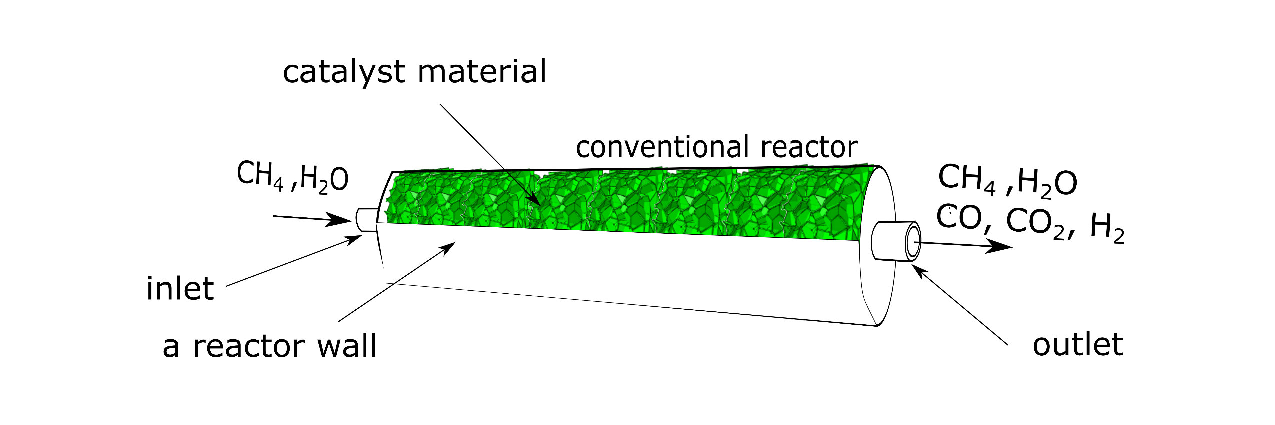
\includegraphics[width=190mm]{conventional-reactor.eps}
\caption{\label{fig:conv_reactor}{Conventional reforming reactor geometry}}
\end{figure}

\begin{figure}[h!]
\centering
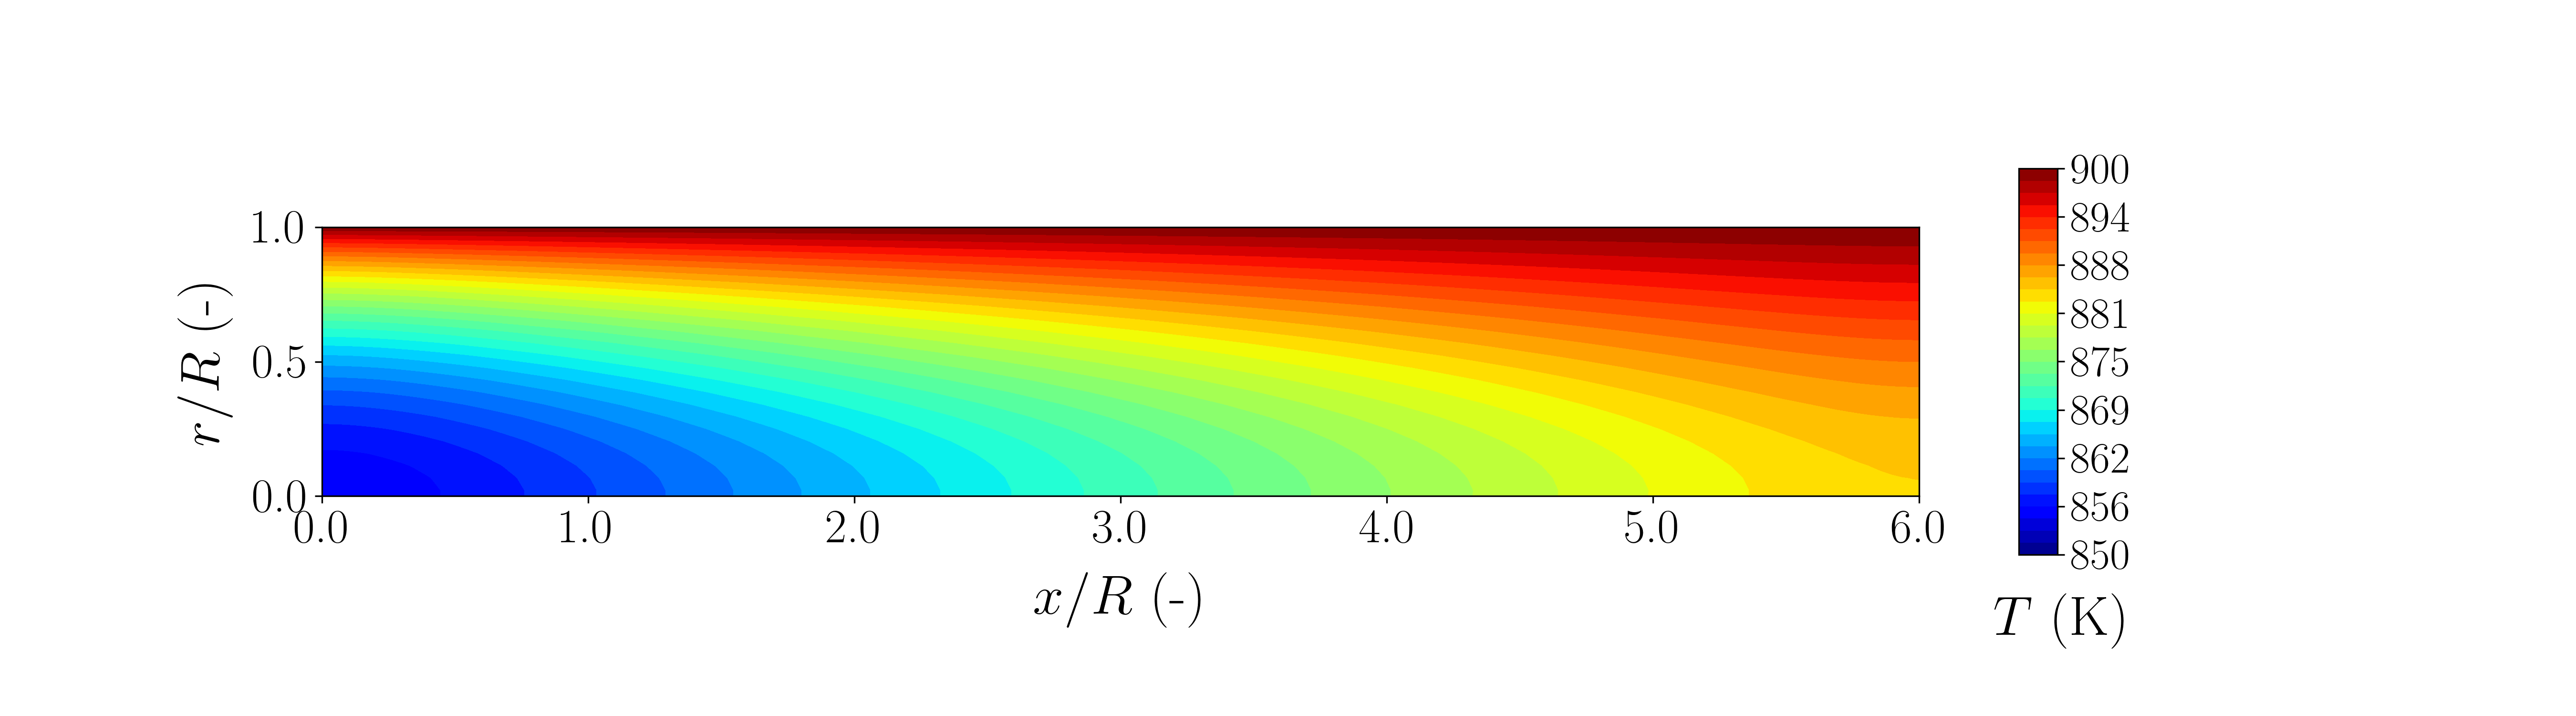
\includegraphics[width=190mm]{ref-Tfield.png}
\caption{\label{fig:conv_reactor_T}{Temperature distribution inside a conventional reforming reactor}}
\end{figure}

The introduction of the macro-pattering concept predicts the division of the catalytic insert in the longitudinal and radial directions. The segments are further filled with either catalytic Ni/YSZ or non-catalytic stainless steel foam. The introduction of the stainless steel foam is expected to allow for a local suppression of the reforming reaction, as the stainless steel is reported to exhibit catalytic at least tow orders of magnitude lower when compared to conventional reforming catalysts \cite{Munster1981, Cheekatamarla2006}. Furthermore, the application of metallic foams is used as a measure of altering the temperature distribution. Metallic foams have a significant heat exchange surface contained in a unit volume. Thus, the stainless steel segments are predicted to enhance the temperature distribution not only due to the reduction of the reaction rate but also due to the superior thermal properties. Following, the application of metallic foams requires the implementation of a heat transfer model exclusive to foam structures \cite{Dai2010}. The extraordinary structure of struts and cells has to be taken into account. The model has to allow for a reliable calculation of heat conduction through the material and heat transfer between the metallic foam and the flowing gas.  The most important parameters required for a relevant description regard structural parameters. The morphology of foam structures is investigated via analysis of digital material representations, generated using an in-house procedure, and further quantified using commercial Avizo software \cite{Pajak2021IJHEa}. Conduction of the structural analysis completes the assumptions necessary for the application of the macro-patterning concept. The strategy is addressed in a few different ways. The original approach predicted the division of the reactor into thirty segments of equal length, in the longitudinal direction \cite{Pajak2018}. Further, the reactor is analyzed considering radial division, resulting in five concentric, porous hollow cylinders, with no division in the longitudinal direction. Two different strategies are proposed for the radial division. The first predicts the construction of cylinders with the exact same width of the inlet surface, while the second predicts the exact same inlet surfaces for the cylinder's inlets. Further, the longitudinal segment division is combined with both radial variants, resulting in another two possible strategies. The exact approach and segments definition process is described in Section \ref{sec:react_geom}. A separate numerical analysis is conducted for each of the described ideas. The general idea behind the macro-patterning concept is illustrated in Fig. \ref{fig:react_pattern}. To allow the achievement of uniform temperature distribution, conduction of proper optimization of the segments' alignment is necessary.  The exact subject of the presented study is to define the most relevant approach to the optimization of the segments distribution in the reactor.


\begin{figure}[h!]
\centering
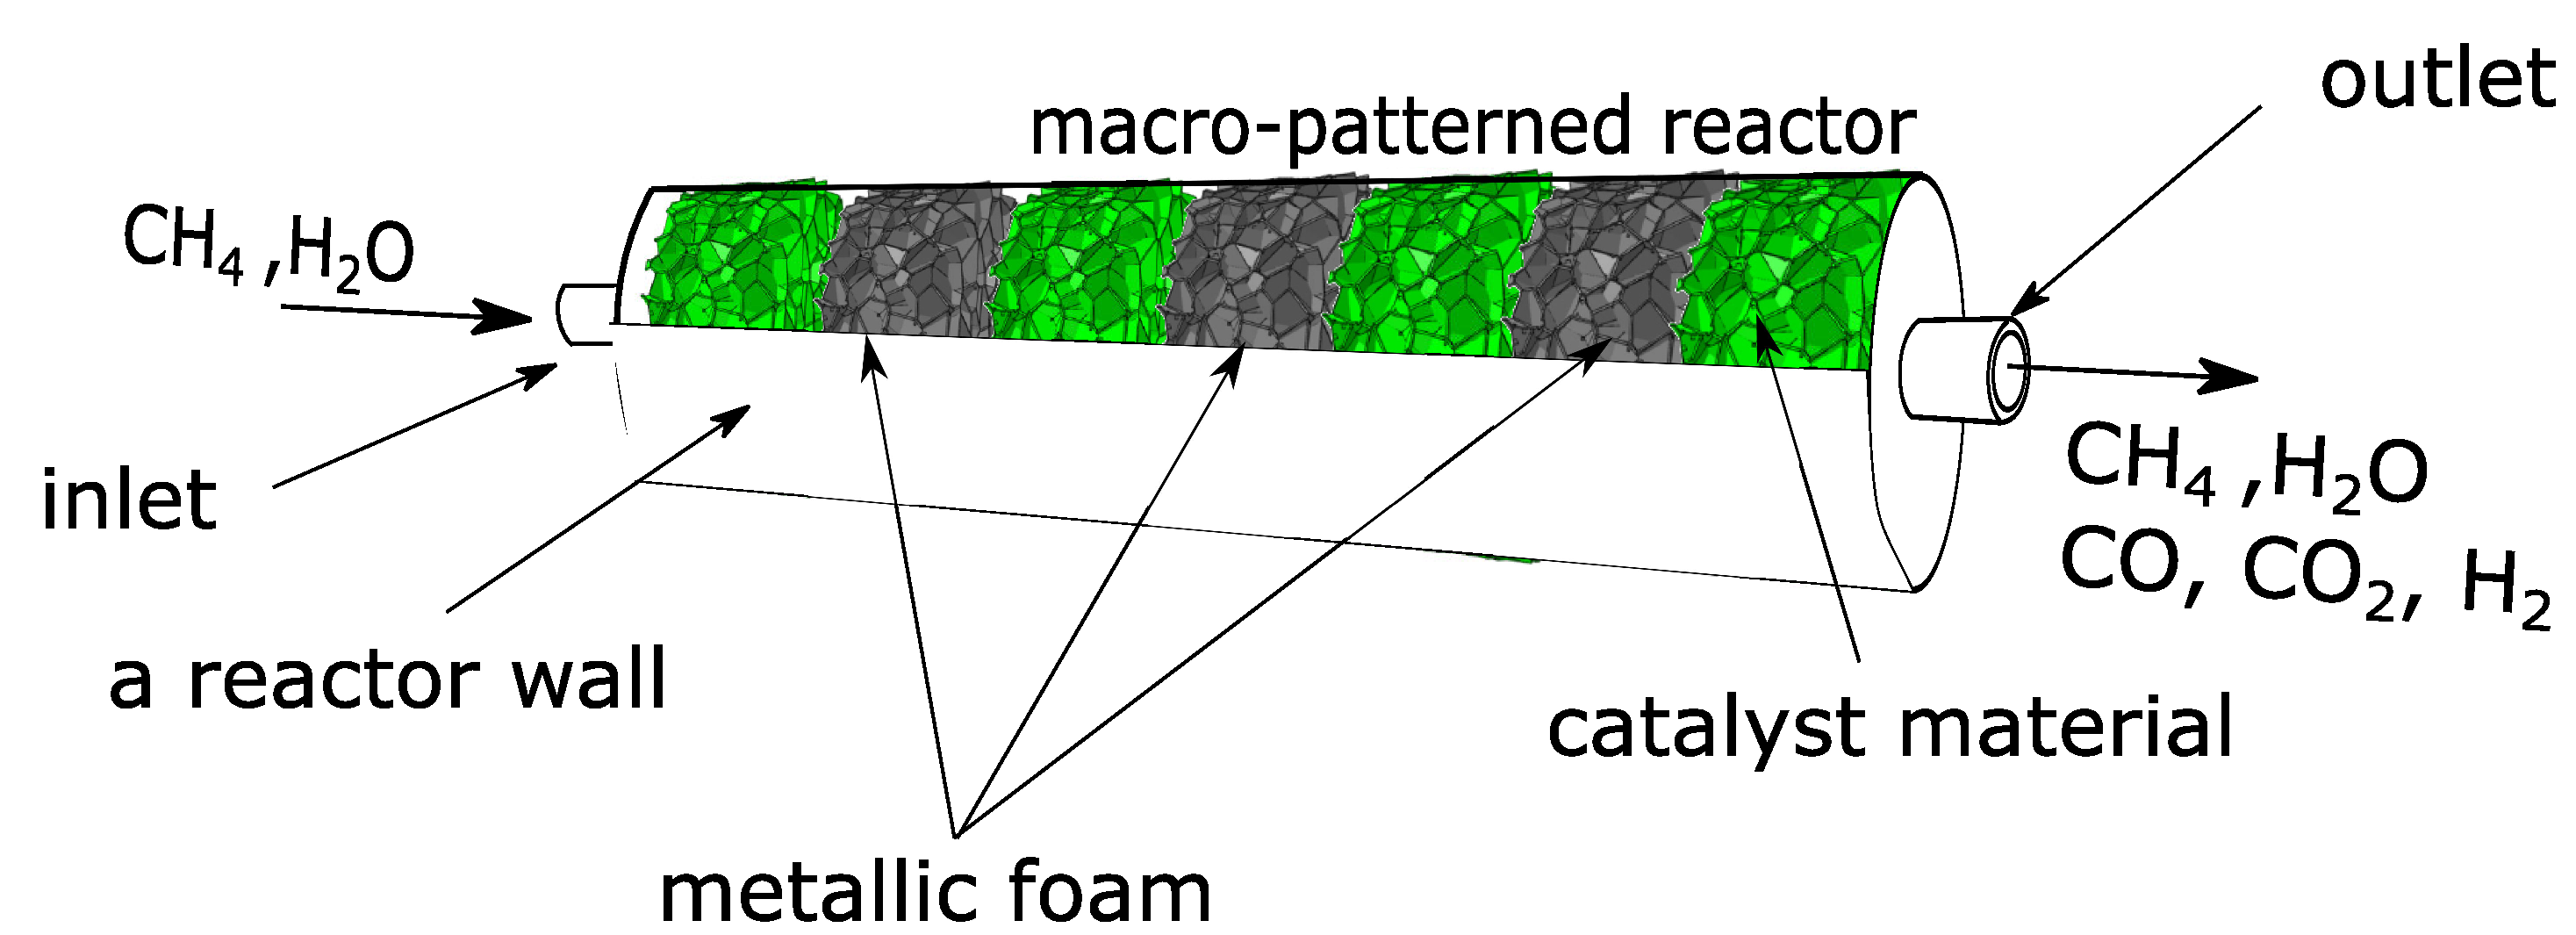
\includegraphics[width=150mm]{macro_geometry.eps}
\caption{\label{fig:react_pattern}{Macro-patterned reactor geometry}}
\end{figure}

\clearpage

Based on the conducted literature review and analysis of the current state of the art, a necessity of optimizing the alignment of the segments is identified. No critical optimization regarding the catalyst distribution in the reforming reactor has been conducted before \cite{Heidebrecht2005, Li2022}. The most advanced investigations are focused on the sensitivity analysis and the adjustment of the process parameters \cite{Rajesh2000, Chen2005, Silva2015}. The optimization procedure is expected to enhance the conditions and effectiveness of an analyzed process or phenomenon. The search for the best solution is conducted through redesigning the conditions, geometry, species composition taking part in the process, etc. The idea of the search for the best solution for a problem has its roots early in the history of mankind. The proofs of the first attempts at the optimization of everyday issues can be found in ancient history.  One of the most recognizable examples is the pursuit of the Greek mathematician Euclid to define the shortest path between two points. Even though the investigation of optimal problems’  solutions started very early, the first proper optimization method was developed by Gauss at the turn of XVIII. Gauss proposed and documented the method of steepest descent used to this day \cite{Curry1944, Meza2010}. Problems regarding optimization can be encountered in each field of science and even in everyday life. The abundance of optimizable phenomena is the reason for the existence of numerous methods and techniques. The procedures may differ in their effectiveness and calculation time \cite{Kusiak2009}. The most conventional approach to the optimization process consists of three steps. The first one predicts the formulation of a proper mathematical model describing be analyzed phenomenon. The second step relies on the definition of fitness functions, which are responsible for the evaluation of the optimization results. The remaining step is the sole optimization procedure itself. The fitness functions are mathematical formulas introduced by the researcher, allowing for deriving a measurable rank for each of the subsequent solutions. The solutions are further evaluated based on the fitness values and the finest is defined as the result of a particular iteration of the optimization procedure \cite{Lange2004}. Basically, the pursuit for the best solution can be brought down to searching for the global minimum or maximum of the fitness function, regarding the considered case. In general, two separate types of the optimization process may be distinguished.  The literature sources define the character of optimization as deterministic or stochastic, depending on the extent of randomness applied to the specific algorithm \cite{Francisco2005}. The deterministic algorithm guarantees convergence in a finite time. However, a certain risk of getting stuck in the local extremum exists. The so-called local extremum trap is a peculiar situation during the analysis of a multi-modal search space. The algorithm falsely recognizes a local extremum as the final step of optimization and terminates the procedure prematurely, as it is unable to break out from the inflection point. Therefore, a deterministic algorithm may be capable of finding a better, but not necessarily the best solution. The reason for the occurrence of the local extremum trap lies down in the principles of the methods. The deterministic algorithms rely on the analysis of the shape of the function’s graph. The stochastic algorithms have a trait for avoiding the local extremum trap, being the introduction of a random factor to the algorithm procedure. Depending on the type of the algorithm, the randomness is introduced to a different extent and in the various parts of specific procedures \cite{Albrecht2003, Spall2012}. The introduction of the random factor serves as a powerful measure for the algorithm to break out from the local extremum, as it enables the procedure to skip freely between parts of the graph if such necessity appears. The selection of a proper optimization procedure character is a vital part of the analysis. To prepare the most robust procedure, a thorough analysis of the optimized problem particularity and conditions has to be conducted. The steam reforming of methane is a widely used technology, but no significant optimization of the process principles has been reported before. The utmost researchers tried to find the best input parameters and alter the operating conditions of the reforming process, like in the research reported by Noureldin et al. or Rajesh et al. \cite{Noureldin2014, Rajesh2000}. However, very few attempts on modifying the reforming unit design and geometry are found. The most advanced research is reported in the article by Heidebrecht and Sundmacher \cite{Heidebrecht2005}. The research regarded optimization of the thermal conditions during a direct internal reforming process inside a molten carbonate fuel cell. The presented model is dimensionless and predicts the division of the fuel cell area into four separate zones, each filled with a catalyst of different densities or activity. Despite the analysis's simplicity, the investigation brought some satisfying results, indicating that the catalyst structure modification is a potentially beneficial solution. Thus, encouraging further investigation of the macro-patterning concept and a deeper analysis of the steam reforming thermal conditions improvement. The subject of the presented thesis's optimization process is to find the best alignment of the catalytic and non-catalytic segments inside the reforming reactor and the segments' morphological parameters. The genetic algorithm is chosen as the optimization technique most suitable for the defined problem \cite{Fouskakis2002}. The genetic algorithm is proven to deal rather effectively with adversely conditioned problems. The algorithm's simplicity and ability to find a global solution are the two main features behind the decision. The genetic algorithm operation is based on evolutionary mechanisms, following the concept of survival of the fittest \cite{Goldberg1989}. In the case of the genetic algorithm, fitness functions are the measure of the evaluation of the specimens and defining the superior ones among the whole population of solutions. The fittest specimens are expected to advance to the next generation and take part in the crossover procedure. The crossover procedure imitates the natural process of gene recombination between the specimens delivering the best results at a certain stage of the optimization process. The algorithm starts its operation by generating an initial population. The specimens being a part of the initial set have the segment parameters entirely randomized. The parameters are further applied to the previously prepared mathematical model used for the calculation of the steam reforming process. Results of this calculation are evaluated by the optimization procedure, assigning a specific fitness for each generated reformer. The amount of processed fuel converted during the reaction and the homogeneity of the temperature field developing inside the reforming reactor are chosen as the most important factors of the analysis. The two features are evaluated based on two separate fitness functions. Regarding the conversion rate, the algorithm aims to maximize the function result, as the level of methane conversion defines the effectiveness of the process. The minimization of the temperature gradients occurring inside the reactor is selected as the second criterion of the analysis. The enhancement of the temperature field distribution inside the reactor is reported to increase the amount of hydrogen contained in the reaction products \cite{Palma2017}. The difference between maximal and minimal temperatures analyzed either locally or globally is chosen as the measure of the magnitude of the gradients.  The previous analyzes indicated that the unification of the temperature field is directly correlated with the difference in the border values of temperature \cite{Pajak2018}. Therefore, the thermal fitness function is minimized by the algorithm. To summarize, the algorithm aims to optimize the design of the macro-patterned reforming reactor catalytic insert. The mutual recombination of the segments’ composition, between specimens among a specific population is expected to deliver results of better quality with each consecutive population. The optimization procedure is continued until optimal values of methane conversion rate and temperature difference are found. Even though a significant part of the algorithm procedure is randomized, the algorithm can not be qualified as a random search method. The genetic algorithms take advantage of the experience gained from preceding calculations to define a new search region, which is expected to contain fitter solutions. Thus, introducing a slight touch of determinism \cite{Goldberg1989}. The presented research regards the optimization of the particular segments distribution and adjustment of morphological parameters, to achieve the highest process efficiency and proper altering of the reforming reaction rate (Chapter \ref{chap:math_model}). Optimization of the given issue is expected to allow the unification of the temperature distribution in the macro-patterned reactor \cite{Pajak2018}. The optimization has to be conducted with respect to maintaining high hydrogen production effectiveness, determining that the problem we are dealing with is a multi-objective optimization. The objectives behave contrarily, as the temperature gradients can only be reduced by limiting the amount of the catalyst used in a particular reactor, which has a consequence in decreasing the methane conversion rate. The less a catalyst is used, the more a reaction rate is diminished. The described problem becomes even more complex if we consider the combinations of possible segment alignments (Chapter \ref{chap:ga}). Some configurations can be falsely recognized as a global optimum when being only an optimal solution in the currently investigated region of the search space. Furthermore, the complexity of the steam reforming simulation results in a considerable computational time, as it combines heat and mass transfer phenomena with the chemical reactions occurring during the process \cite{Brus2012}. Thus, designing a robust optimization procedure is an arduous task. Due to the limited computational capabilities and high cost of the simulation, a fully conventional approach to segment distribution optimization is not possible. The number of specimens in a single generation is exceptionally limited, to allow the computations to deliver results in a finite time. The unconventional approach to the genetic algorithm induces a necessity for a comprehensive investigation of the algorithm conditions and parameters. A complete sensitivity analysis is conducted as the part of the research, to ensure the most suitable optimization strategy, considering the steam reforming reaction.


\clearpage
\section{Numerical analysis}
\label{sec:num_analysis}

%\begin{figure}[h!]
%\centering
%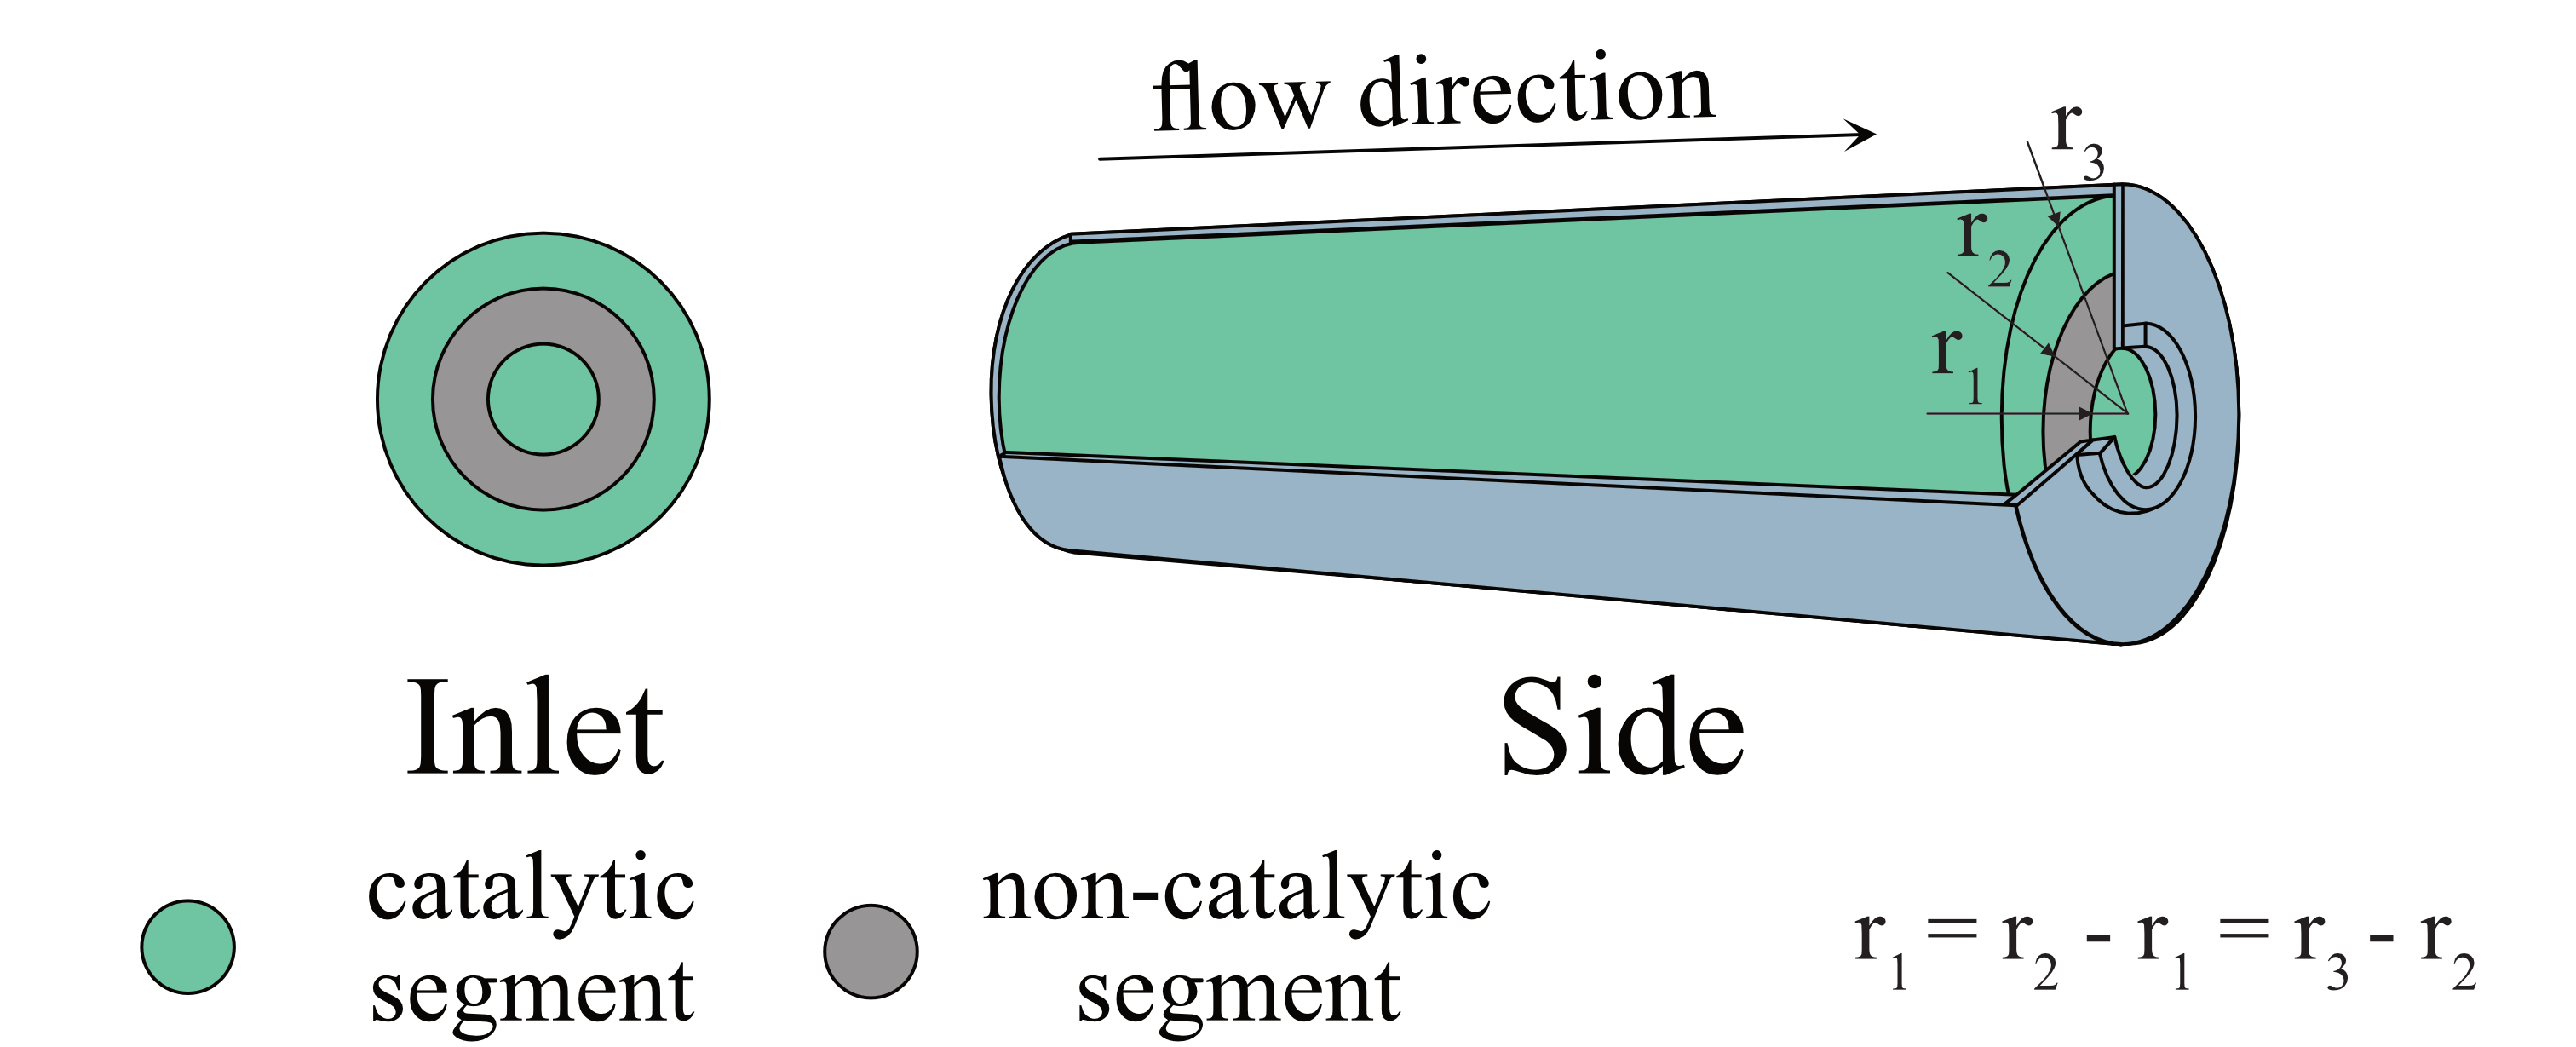
\includegraphics[width=120mm]{5seg.png}
%\caption{\label{fig:5seg}Catalytic insert division strategy I}
%\end{figure}
%
%
%\paragraph{Thermal fitness 80 \%, methane conversion 20 \%} \hspace{0pt} \\
%\noindent 
%
%\begin{figure}[h!]
%\centering
%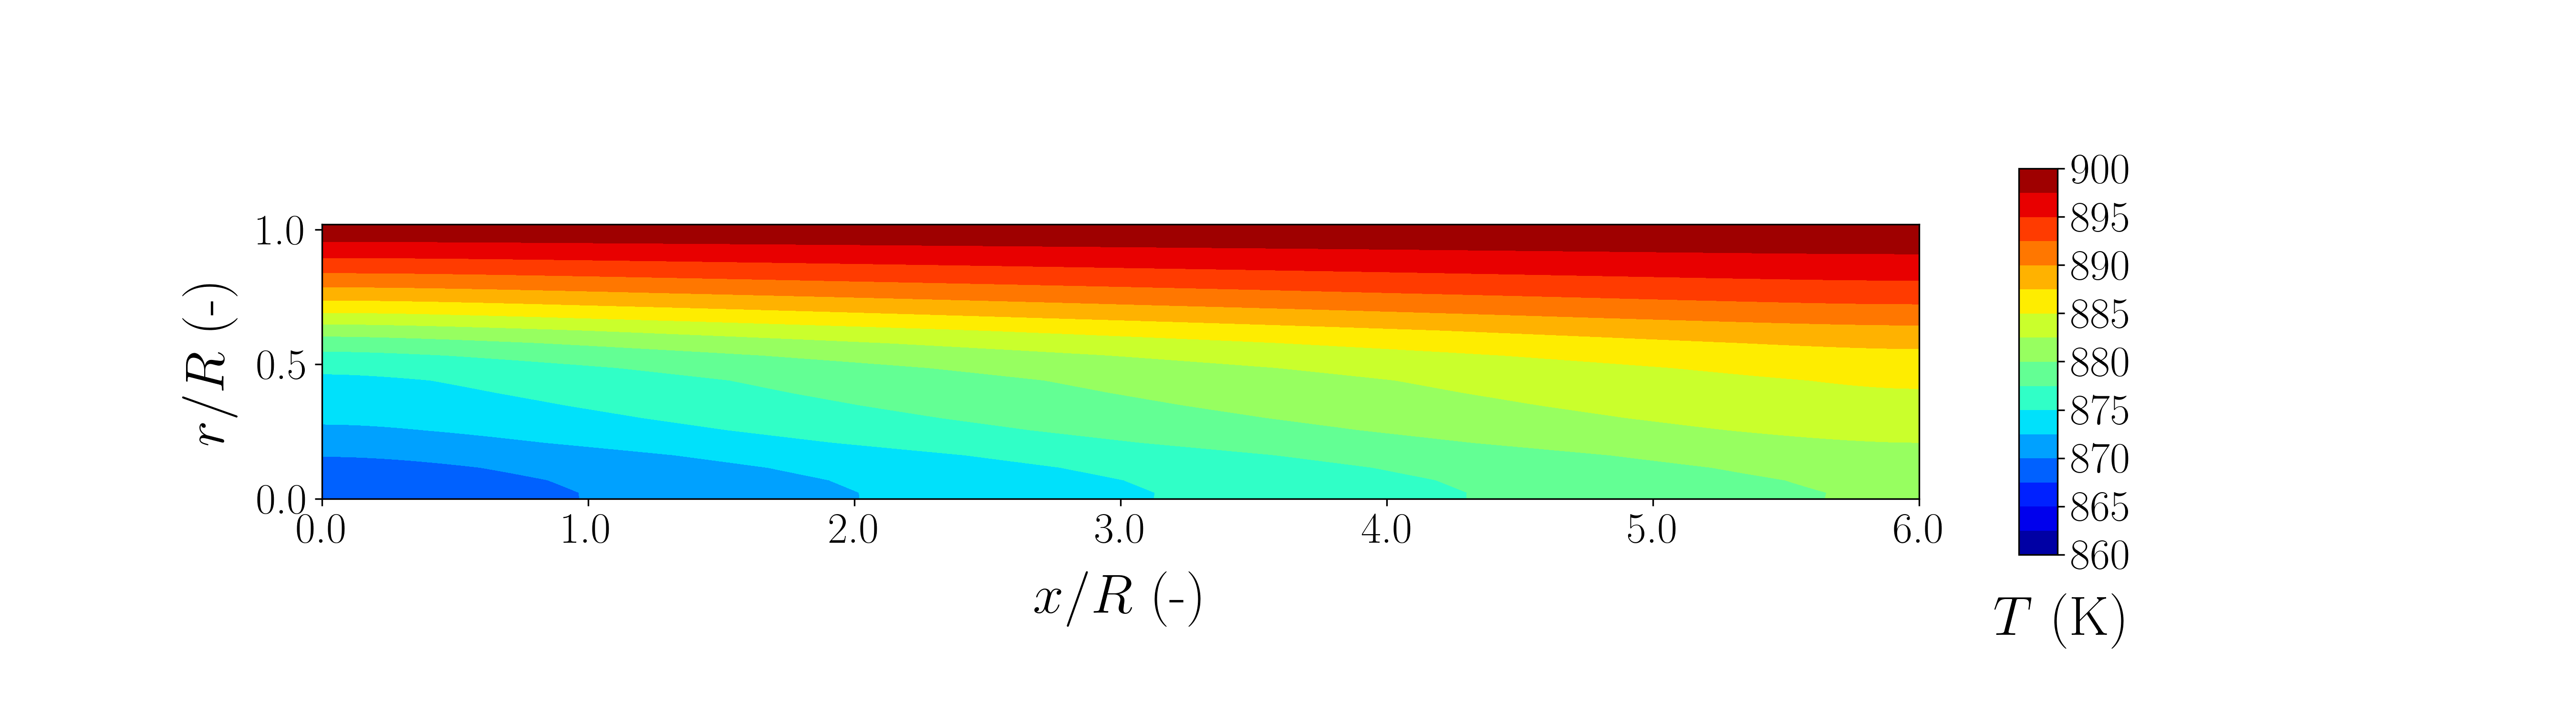
\includegraphics[width=190mm]{results/5/20C_80T/GEN1-TFIELD.png}
%\caption{\label{fig:5R2080G1-TField} Strategy I - Temperature field distribution - 1$^{\rm{st}}$ generation ($w_{\rm{CH_4}} = 0.2, w_T = 0.8$, $T_{\rm{in}}$ = 900 K, $u_{\rm{in}}$ = 0.15 m s$^{-1}$, $SC$ = 2.0)}
%\end{figure}
%
%\begin{figure}[h!]
%\centering
%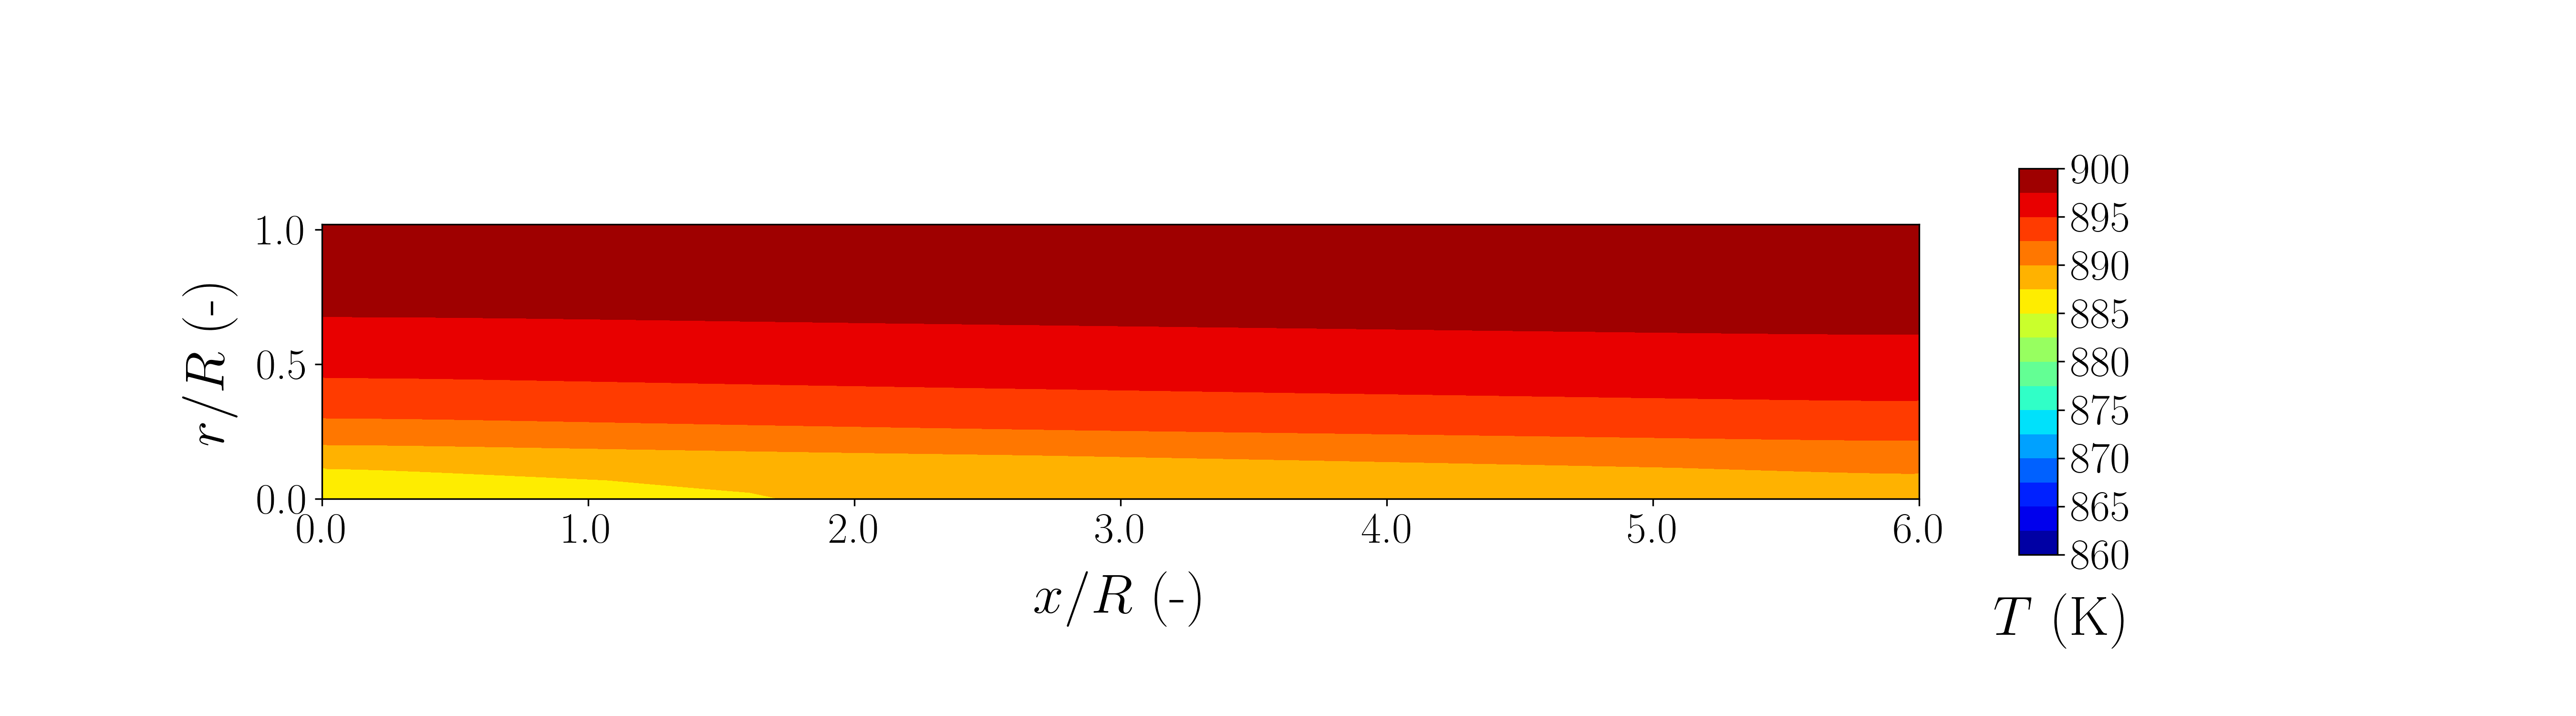
\includegraphics[width=190mm]{results/5/20C_80T/GEN15-TFIELD.png}
%\caption{\label{fig:5R2080G15-TField} Strategy I - Temperature field distribution - 15$^{\rm{th}}$ generation ($w_{\rm{CH_4}} = 0.2, w_T = 0.8$, $T_{\rm{in}}$ = 900 K, $u_{\rm{in}}$ = 0.15 m s$^{-1}$, $SC$ = 2.0)}
%\end{figure}
%
%\begin{figure}[h!]
%\centering
%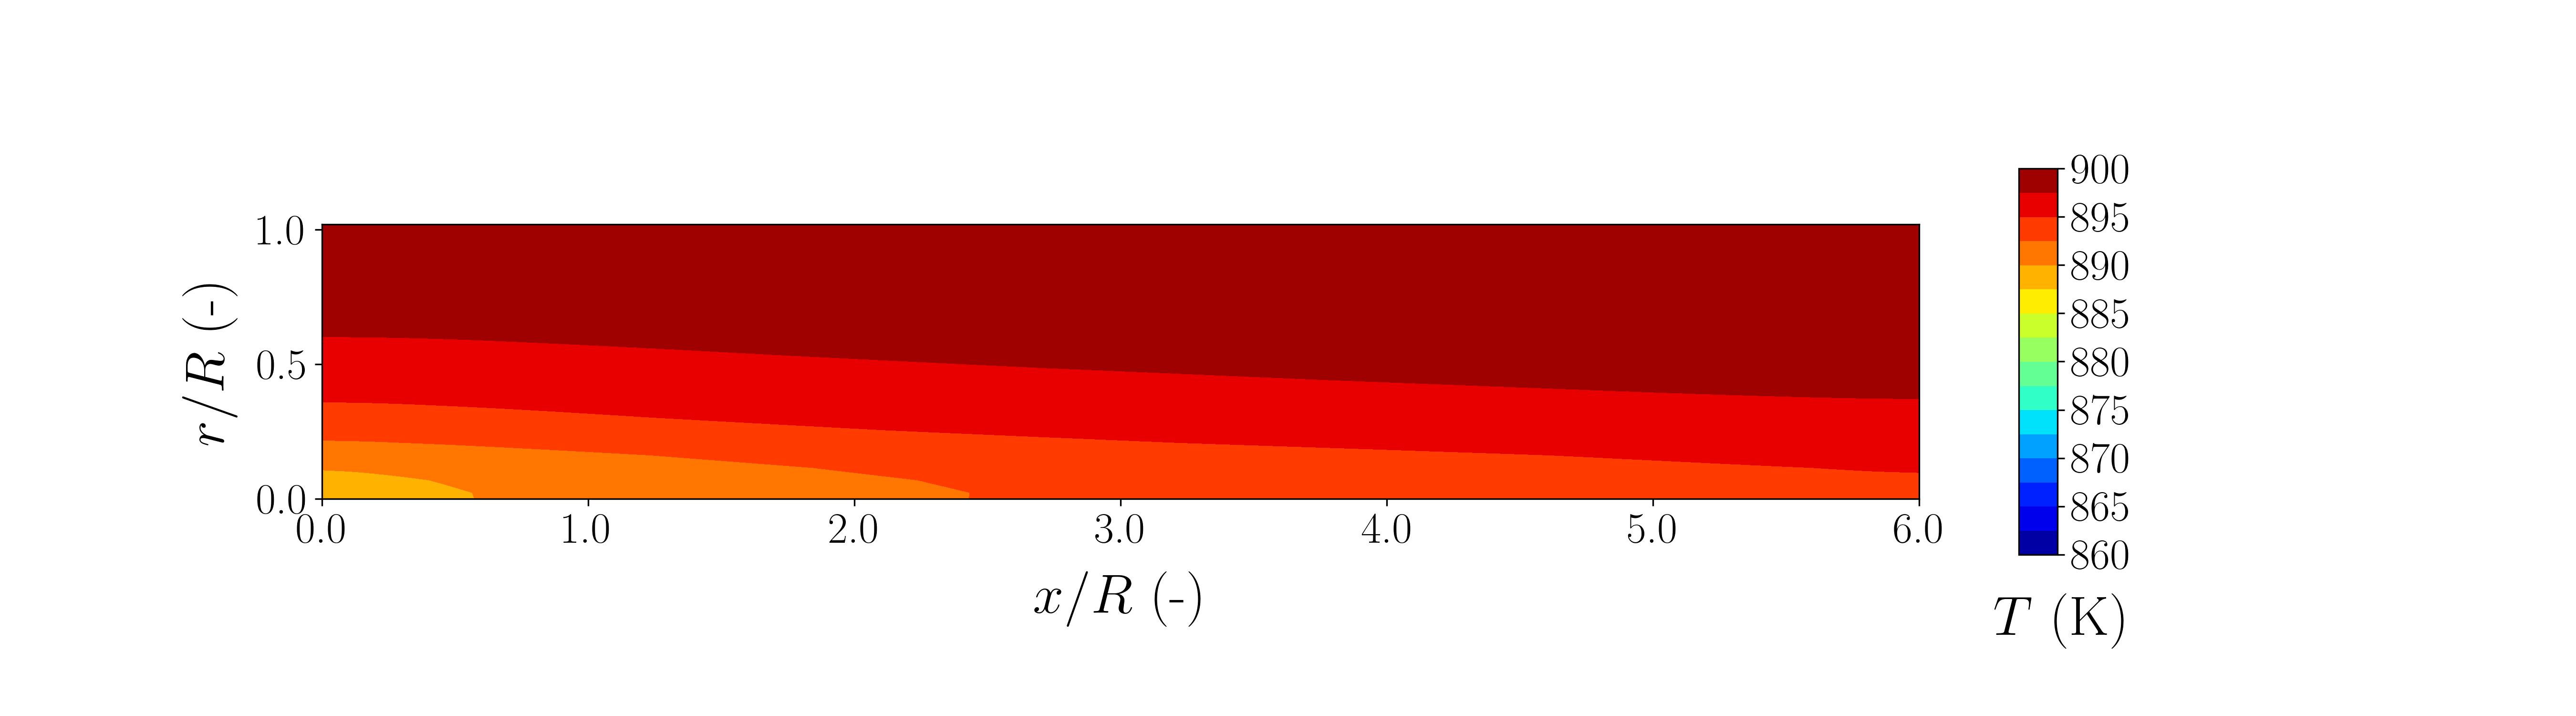
\includegraphics[width=190mm]{results/5/20C_80T/GEN30-TFIELD.png}
%\caption{\label{fig:5R2080G30-TField} Strategy I - Temperature field distribution - 30$^{\rm{th}}$ generation ($w_{\rm{CH_4}} = 0.2, w_T = 0.8$, $T_{\rm{in}}$ = 900 K, $u_{\rm{in}}$ = 0.15 m s$^{-1}$, $SC$ = 2.0)}
%\end{figure}
%
%
%\begin{figure}[h!]
%\centering
%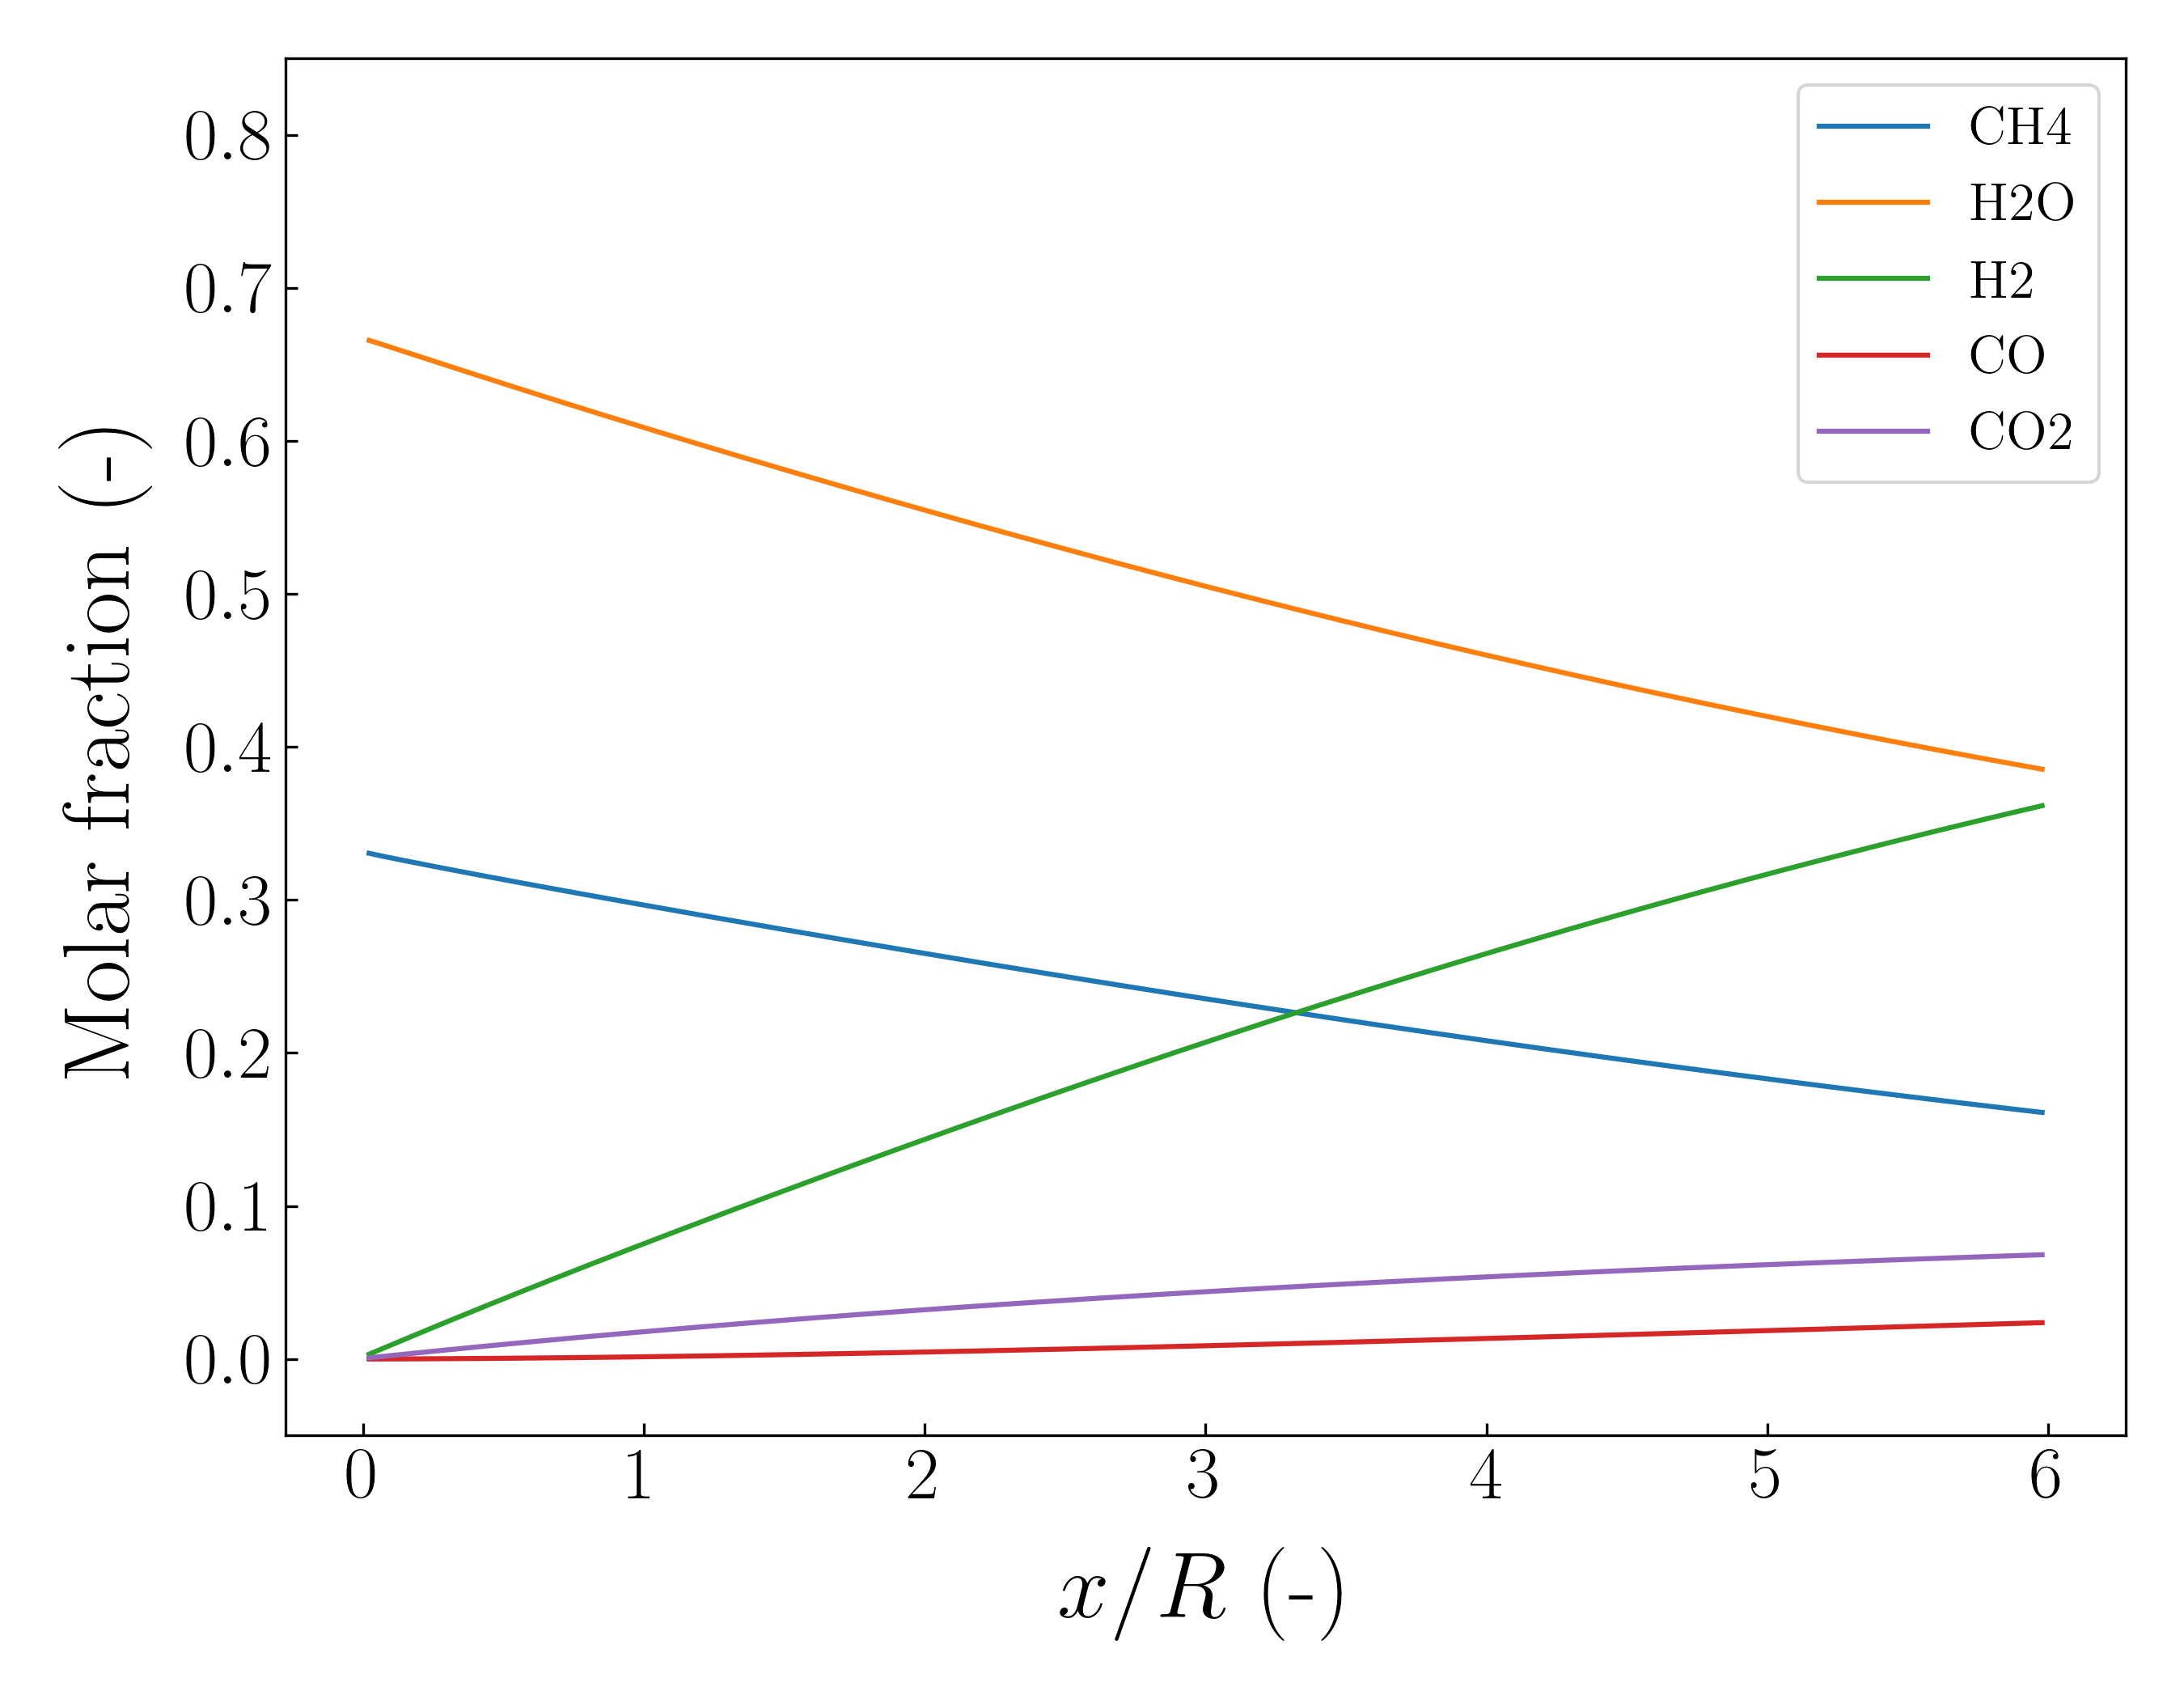
\includegraphics[width=80mm]{results/5/20C_80T/GEN1-AVG.png}
%\caption{\label{fig:5R2080G1-avg} Strategy I - Radius-averaged molar fractions - 1$^{\rm{st}}$ generation ($w_{\rm{CH_4}} = 0.2, w_T = 0.8$, $T_{\rm{in}}$ = 900 K, $u_{\rm{in}}$ = 0.15 m s$^{-1}$, $SC$ = 2.0)}
%\end{figure}
%
%\begin{figure}[h!]
%\centering
%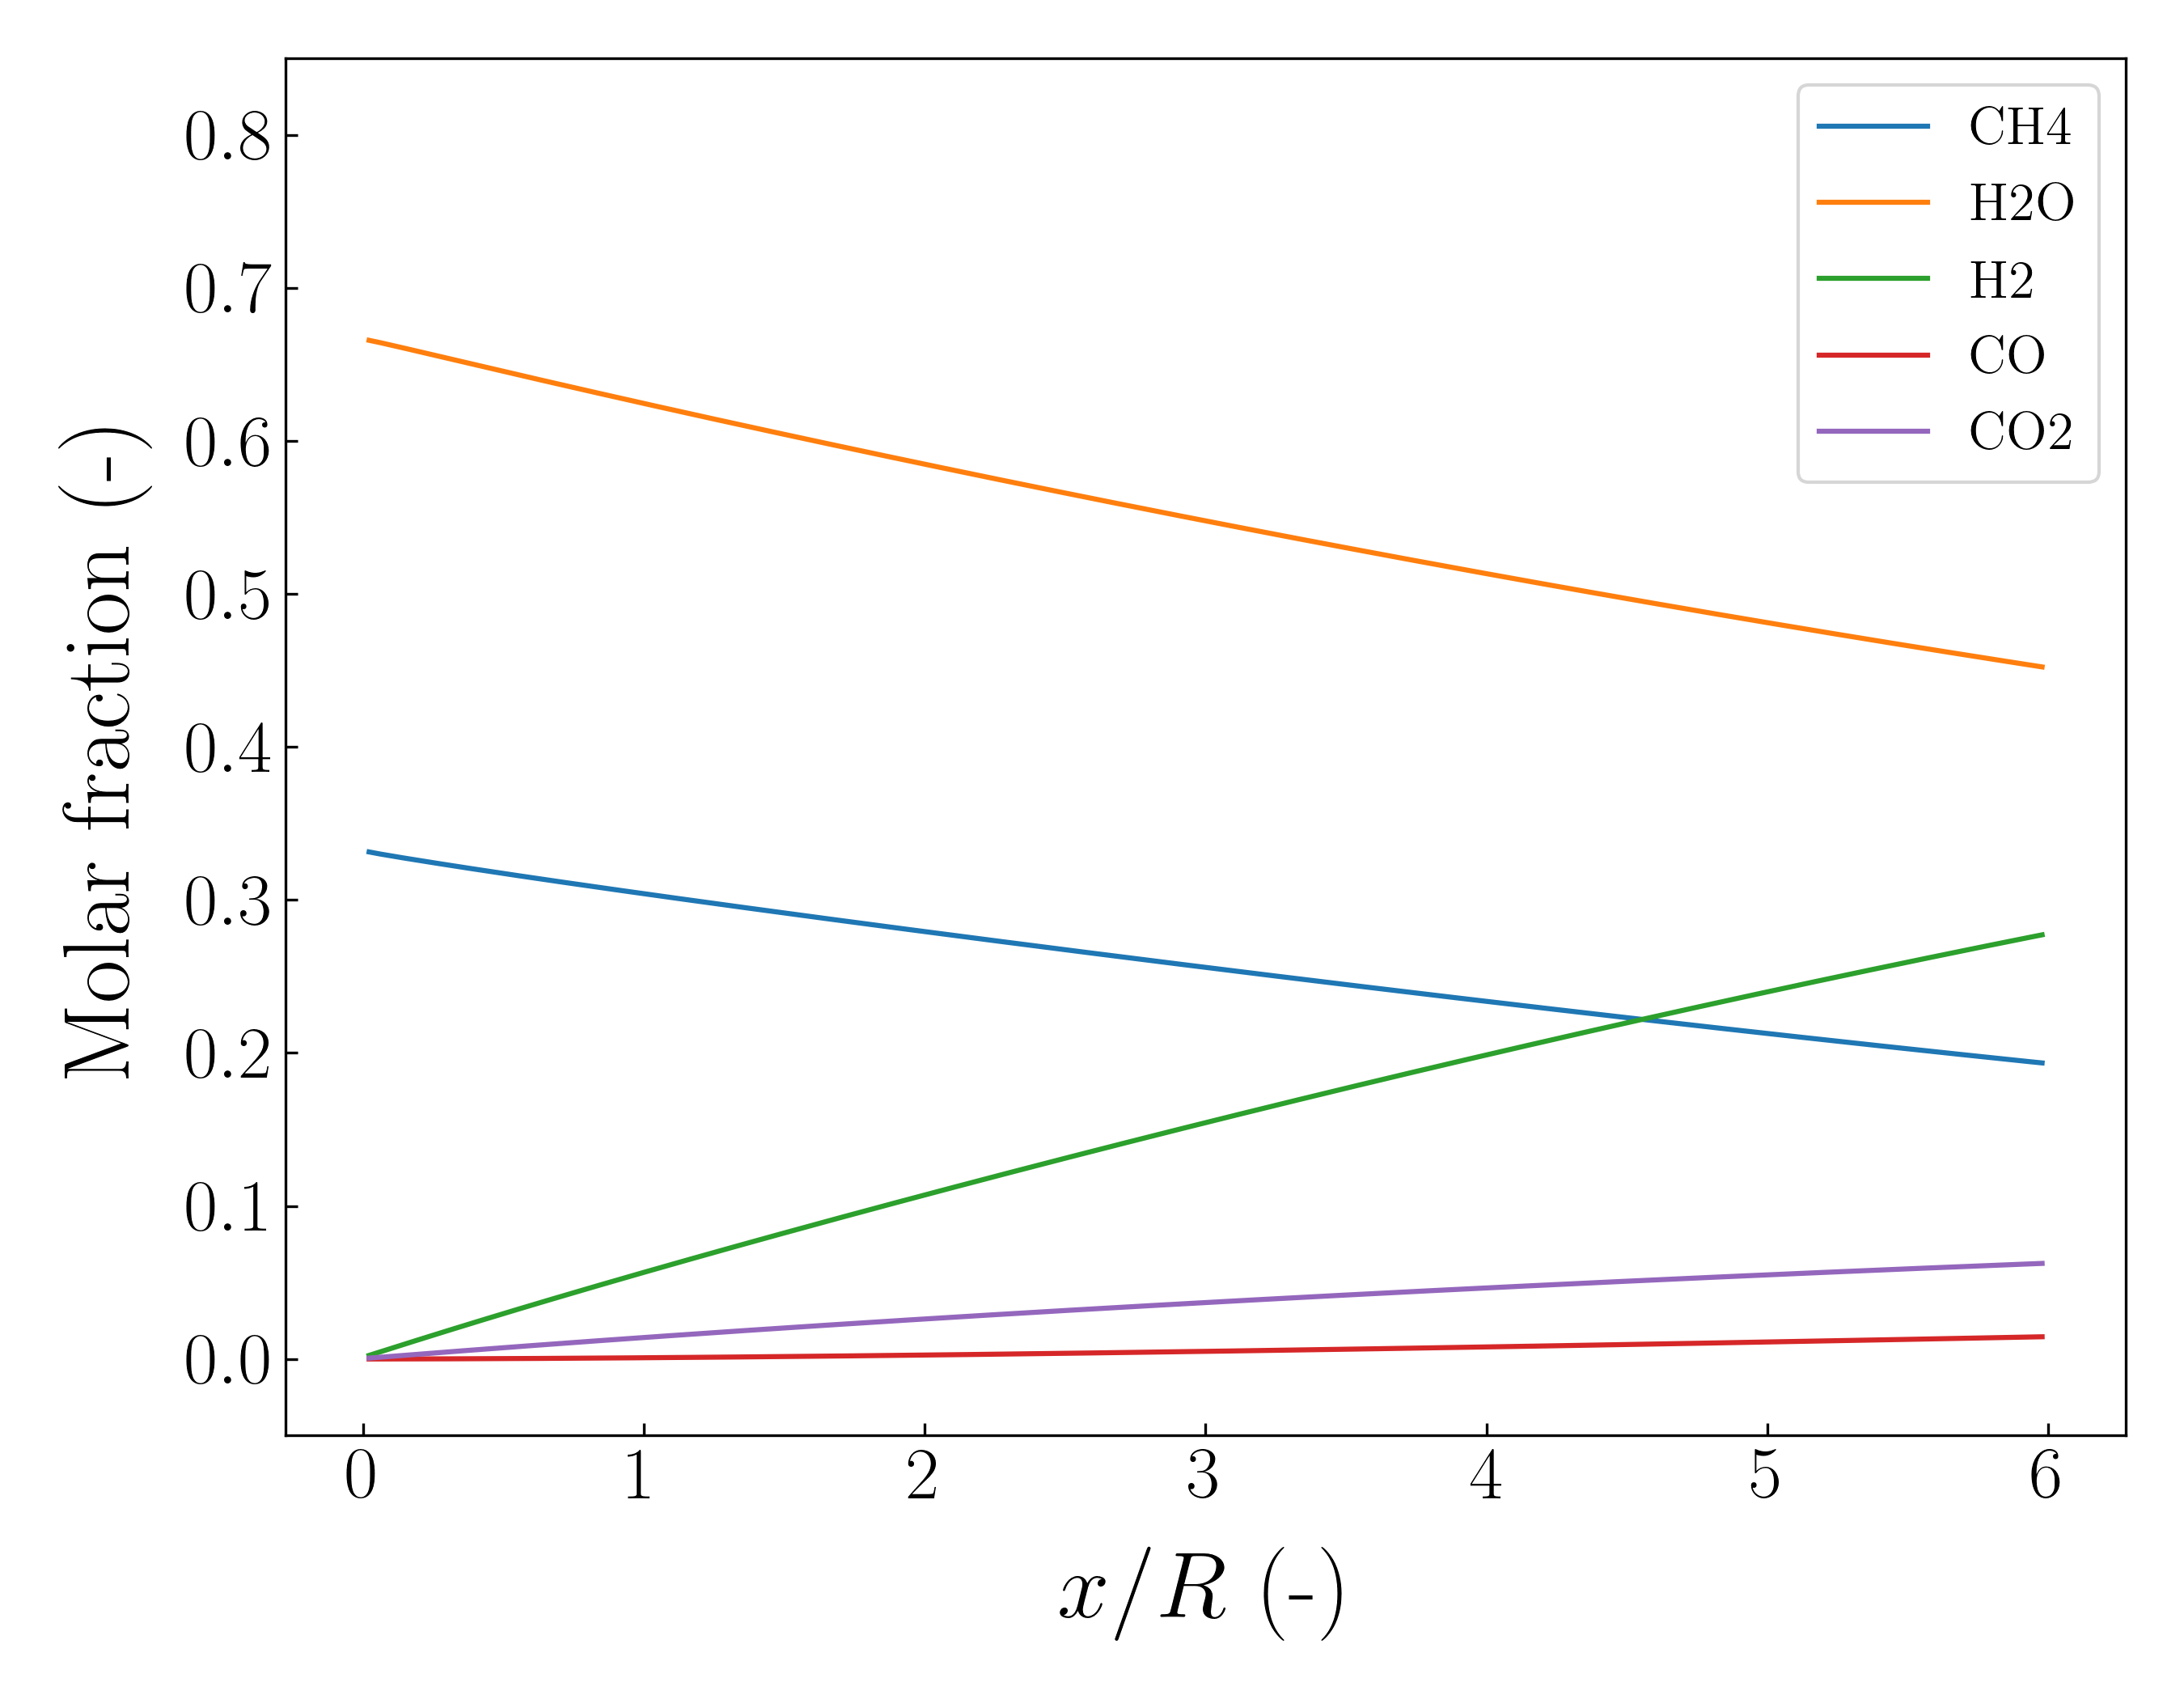
\includegraphics[width=80mm]{results/5/20C_80T/GEN15-AVG.png}
%\caption{\label{fig:5R2080G15-avg} Strategy I - Radius-averaged molar fractions - 15$^{\rm{th}}$ generation ($w_{\rm{CH_4}} = 0.2, w_T = 0.8$, $T_{\rm{in}}$ = 900 K, $u_{\rm{in}}$ = 0.15 m s$^{-1}$, $SC$ = 2.0)}
%\end{figure}
%
%\begin{figure}[h!]
%\centering
%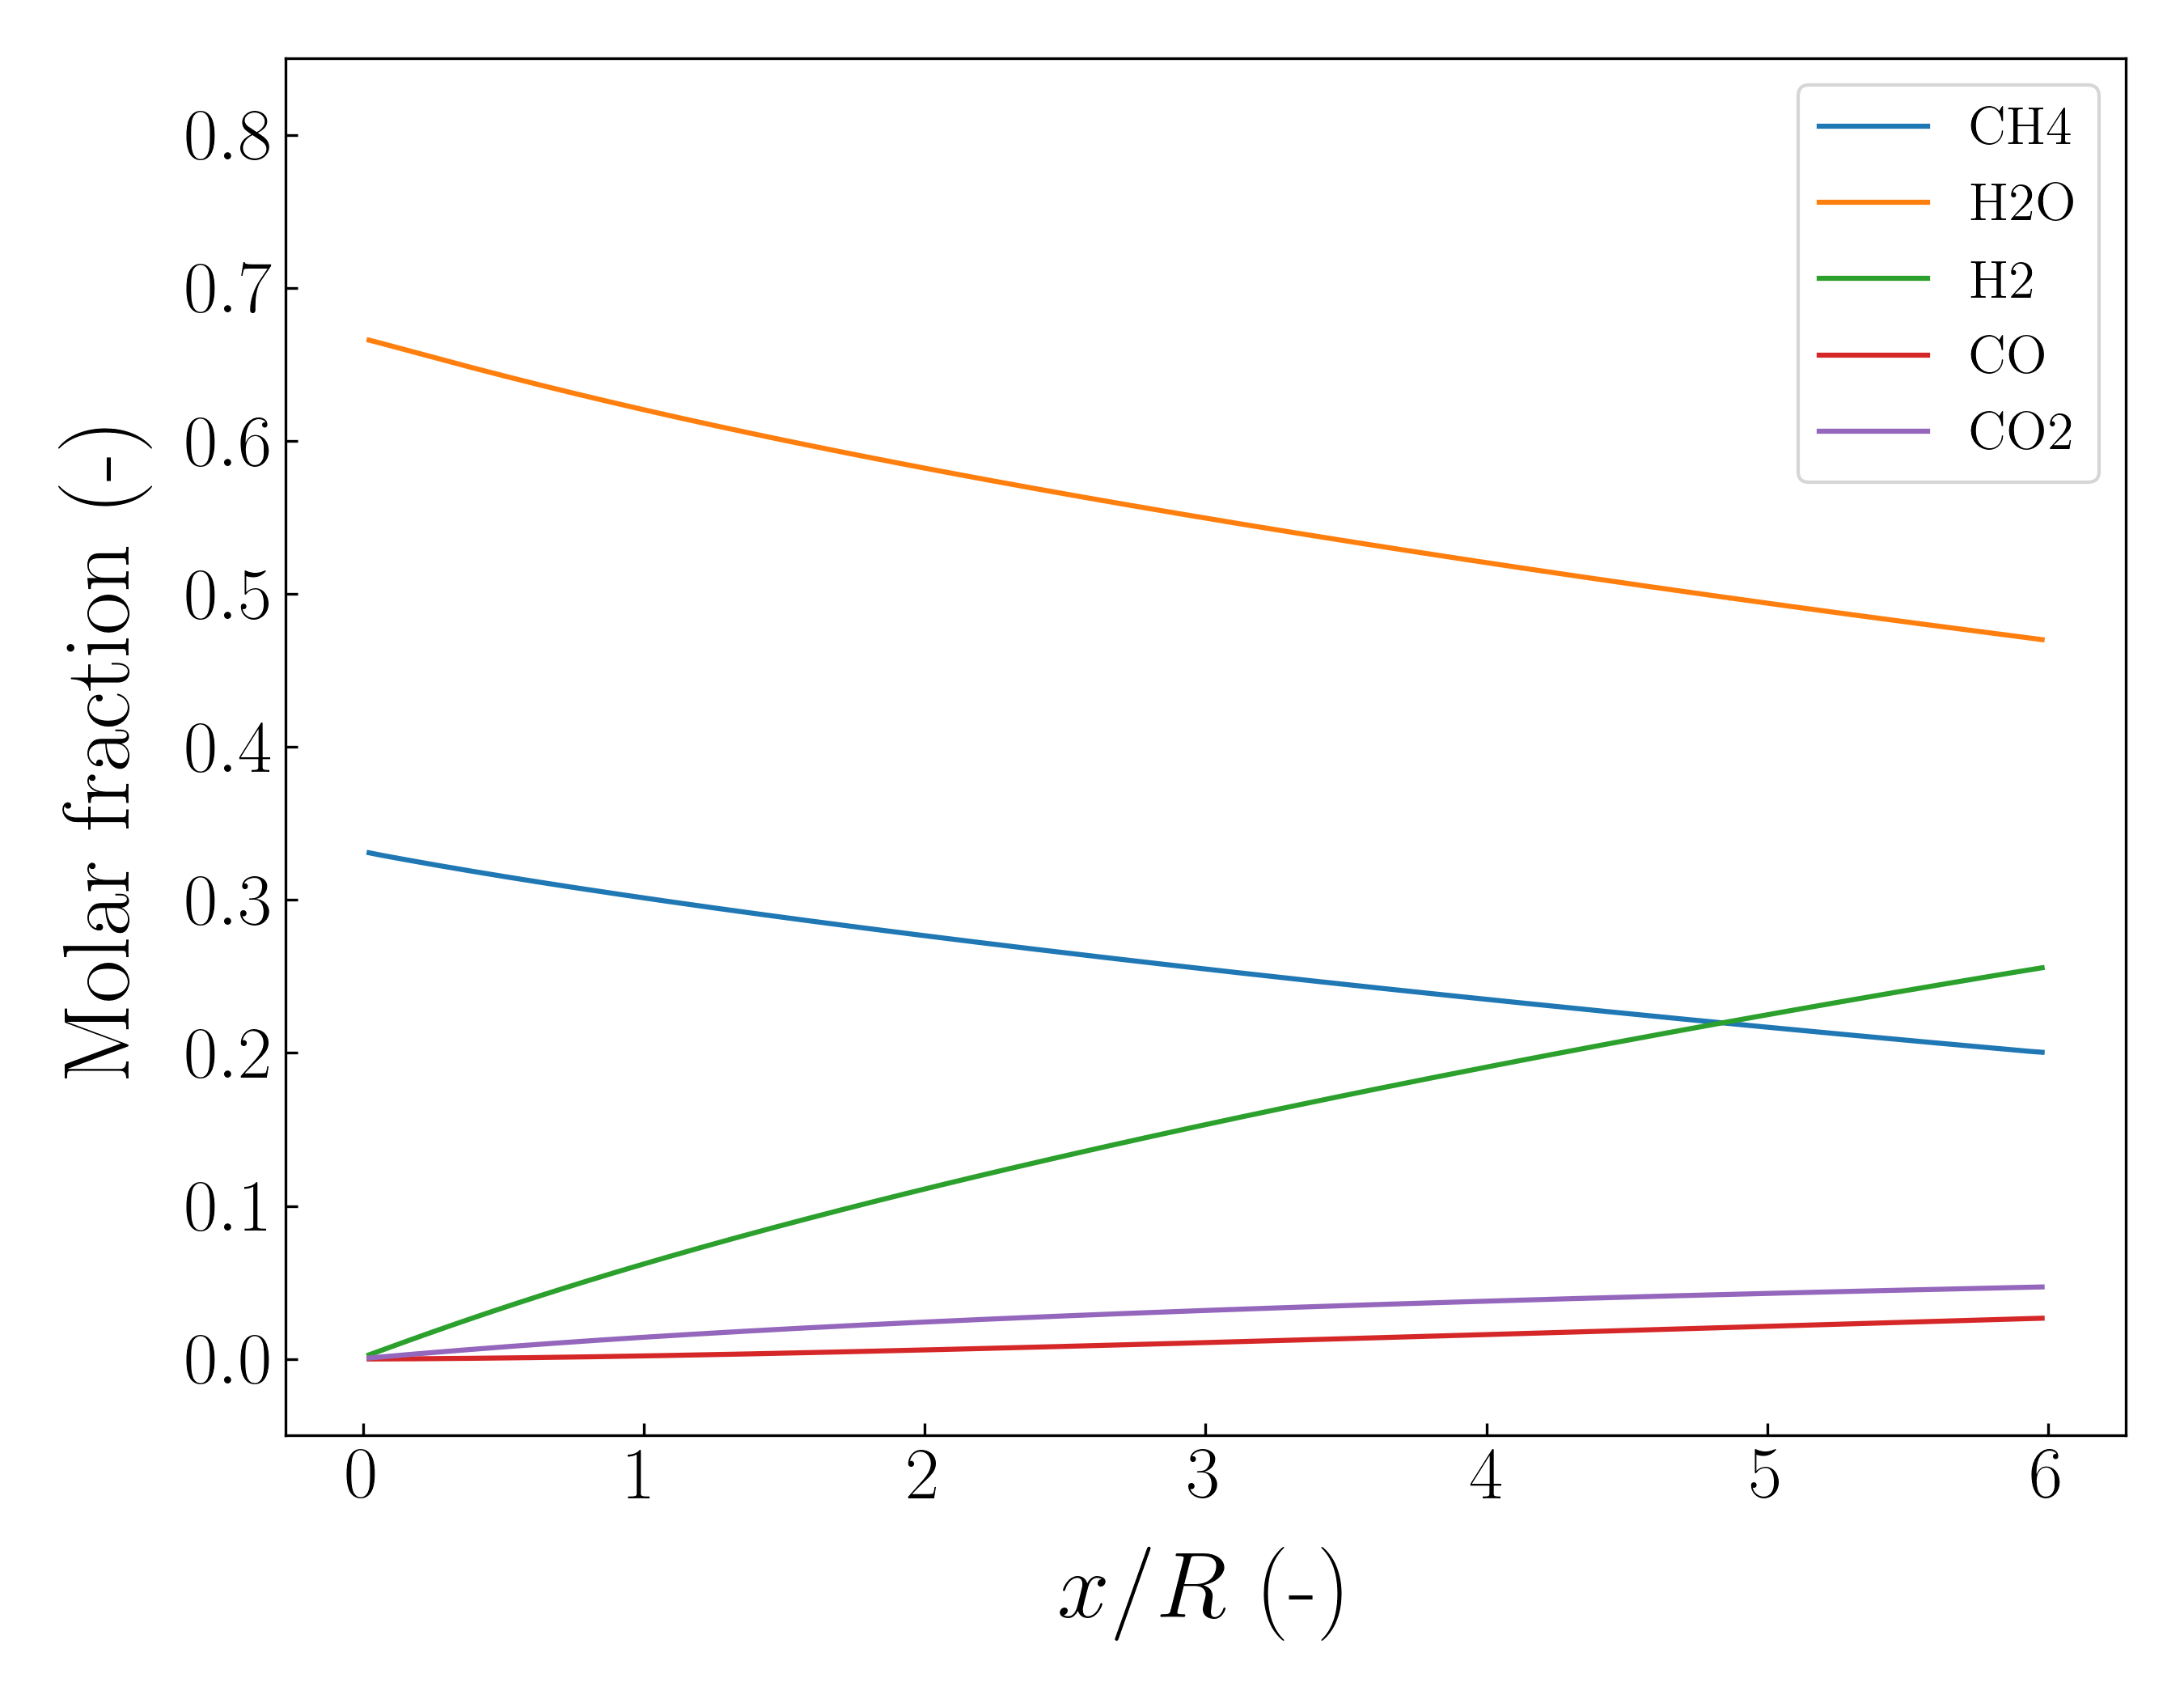
\includegraphics[width=80mm]{results/5/20C_80T/GEN30-AVG.png}
%\caption{\label{fig:5R2080G30-avg} Strategy I - Radius-averaged molar fractions -  30$^{\rm{th}}$ generation ($w_{\rm{CH_4}} = 0.2, w_T = 0.8$, $T_{\rm{in}}$ = 900 K, $u_{\rm{in}}$ = 0.15 m s$^{-1}$, $SC$ = 2.0)}
%\end{figure}
%
%\begin{figure}[h!]
%\centering
%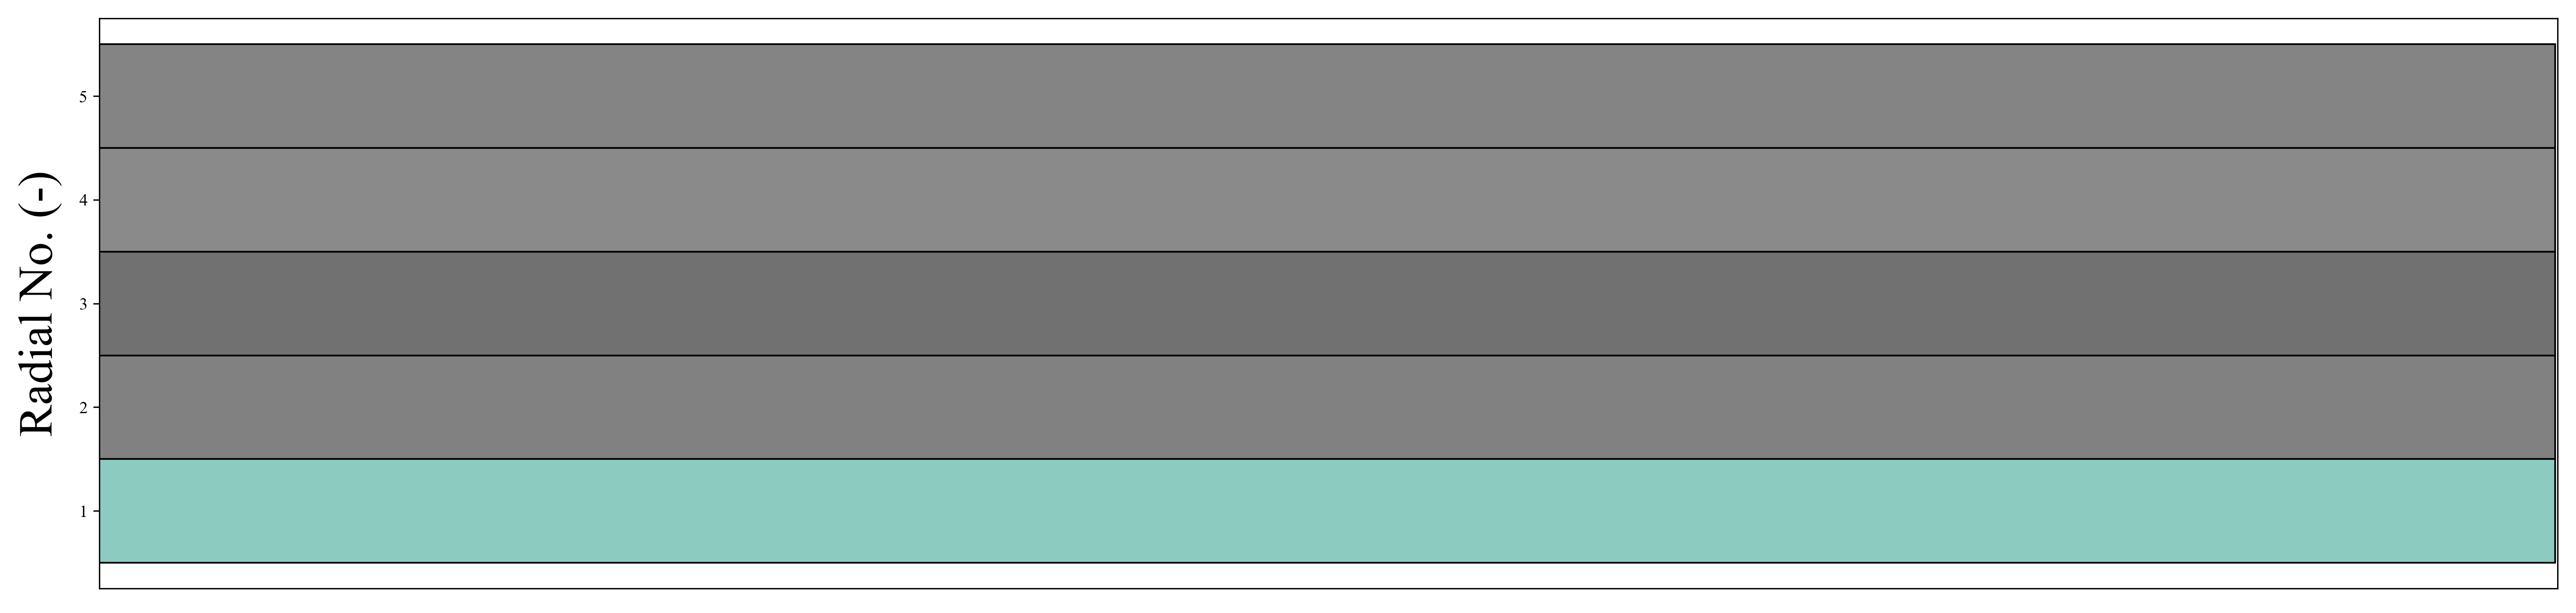
\includegraphics[width=120mm]{results/segments/5seg/20C80T/seg.png}
%\caption{\label{fig:30L6040G1-TField} Strategy I - Segments distribution for 30$^{\rm{th}}$ generation ($w_{\rm{CH_4}} = 0.2, w_T = 0.8$, $T_{\rm{in}}$ = 900 K, $u_{\rm{in}}$ = 0.15 m s$^{-1}$, $SC$ = 2.0)}
%\end{figure}
%
%\begin{figure}[h!]
%\centering
%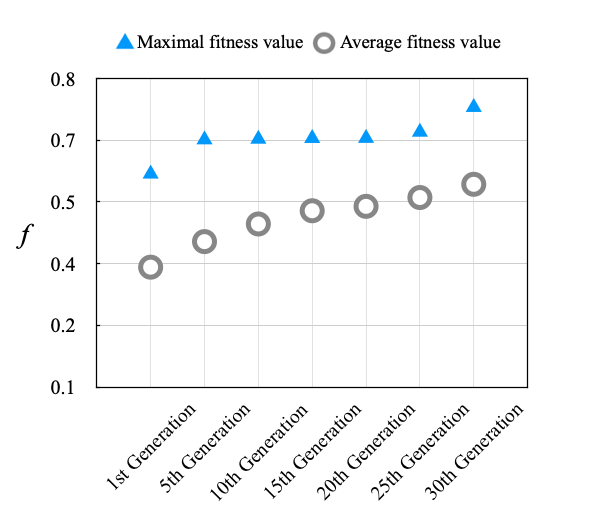
\includegraphics[width=100mm]{results/5/20C_80T.png}
%\caption{\label{fig:5R2080G-fitness} Strategy I - Fitness analysis throughout successive populations ($w_{\rm{CH_4}} = 0.2, w_T = 0.8$, $T_{\rm{in}}$ = 900 K, $u_{\rm{in}}$ = 0.15 m s$^{-1}$, $SC$ = 2.0)}
%\end{figure}
%
%
%
%\clearpage
%
%
%
%\paragraph{Thermal fitness 60 \%, methane conversion 40 \%} \hspace{0pt} \\
%\noindent 
%
%
%\begin{figure}[h!]
%\centering
%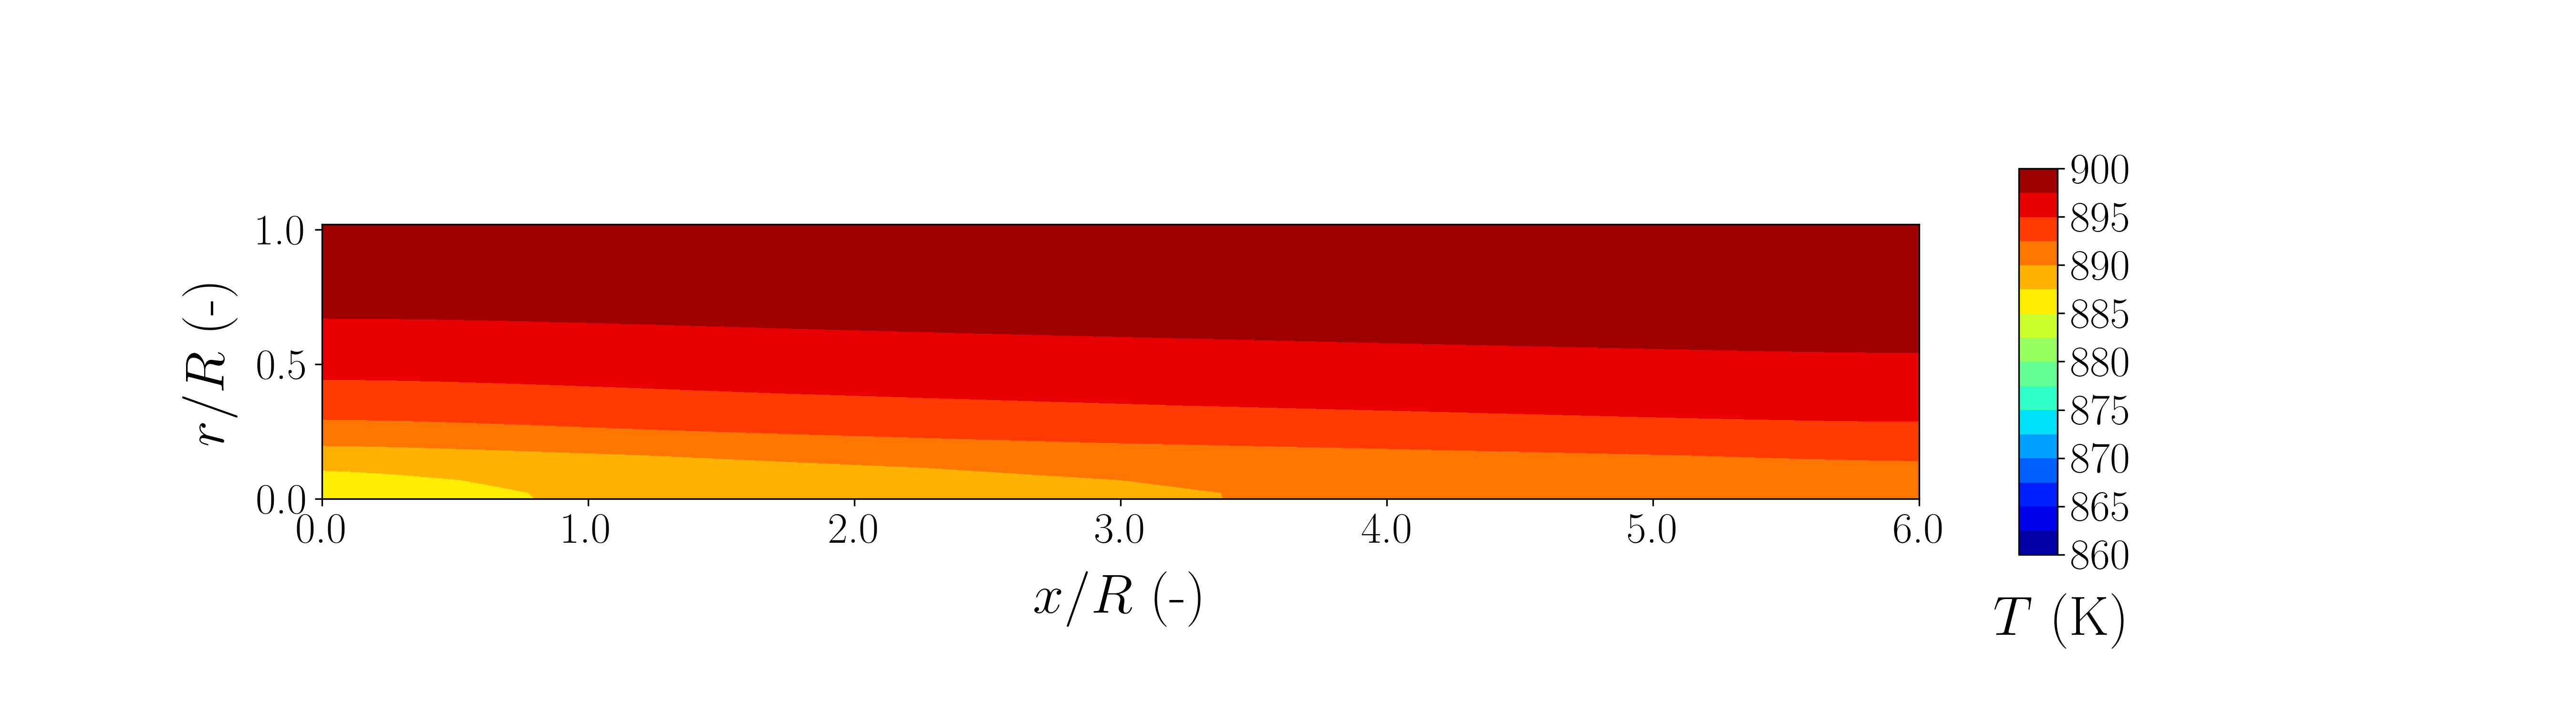
\includegraphics[width=190mm]{results/5/40C_60T/GEN1-TFIELD.png}
%\caption{\label{fig:5R4060G1-TField} Strategy I - Temperature field distribution - 1$^{\rm{st}}$ generation ($w_{\rm{CH_4}} = 0.4, w_T = 0.6$, $T_{\rm{in}}$ = 900 K, $u_{\rm{in}}$ = 0.15 m s$^{-1}$, $SC$ = 2.0)}
%\end{figure}
%
%\begin{figure}[h!]
%\centering
%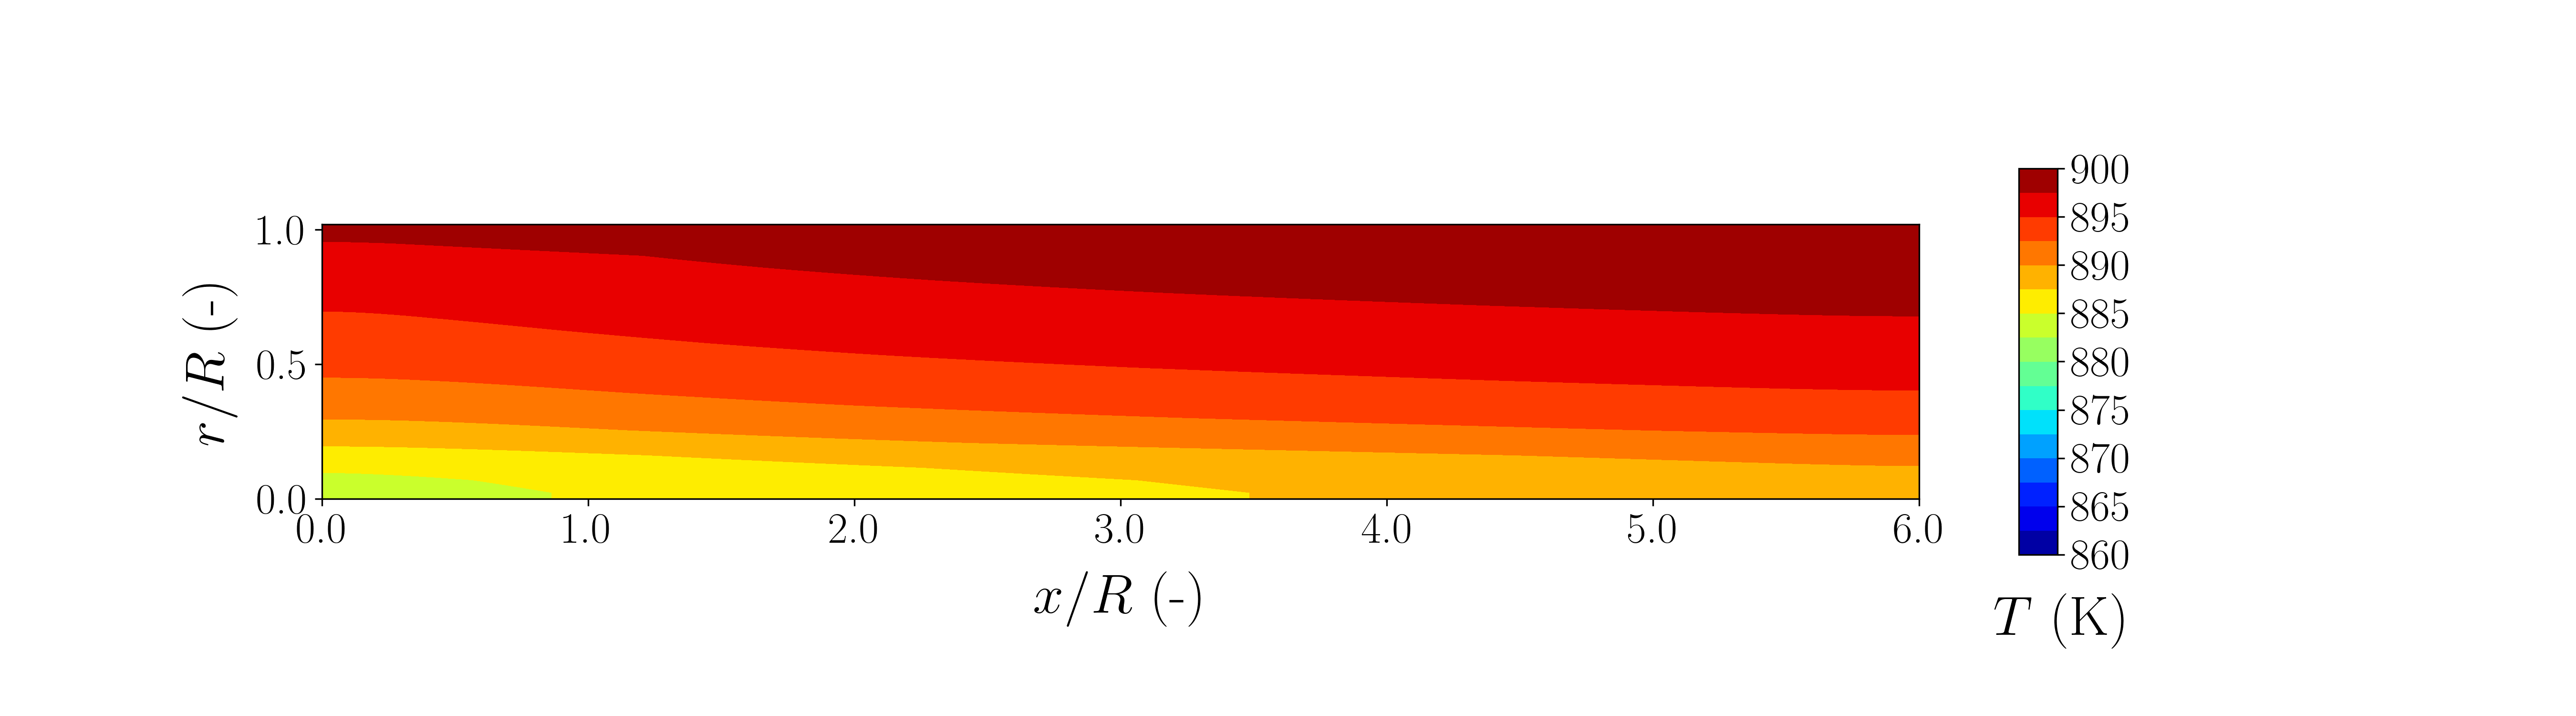
\includegraphics[width=190mm]{results/5/40C_60T/GEN15-TFIELD.png}
%\caption{\label{fig:5R4060G15-TField} Strategy I - Temperature field distribution - 15$^{\rm{th}}$ generation ($w_{\rm{CH_4}} = 0.4, w_T = 0.6$, $T_{\rm{in}}$ = 900 K, $u_{\rm{in}}$ = 0.15 m s$^{-1}$, $SC$ = 2.0)}
%\end{figure}
%
%\begin{figure}[h!]
%\centering
%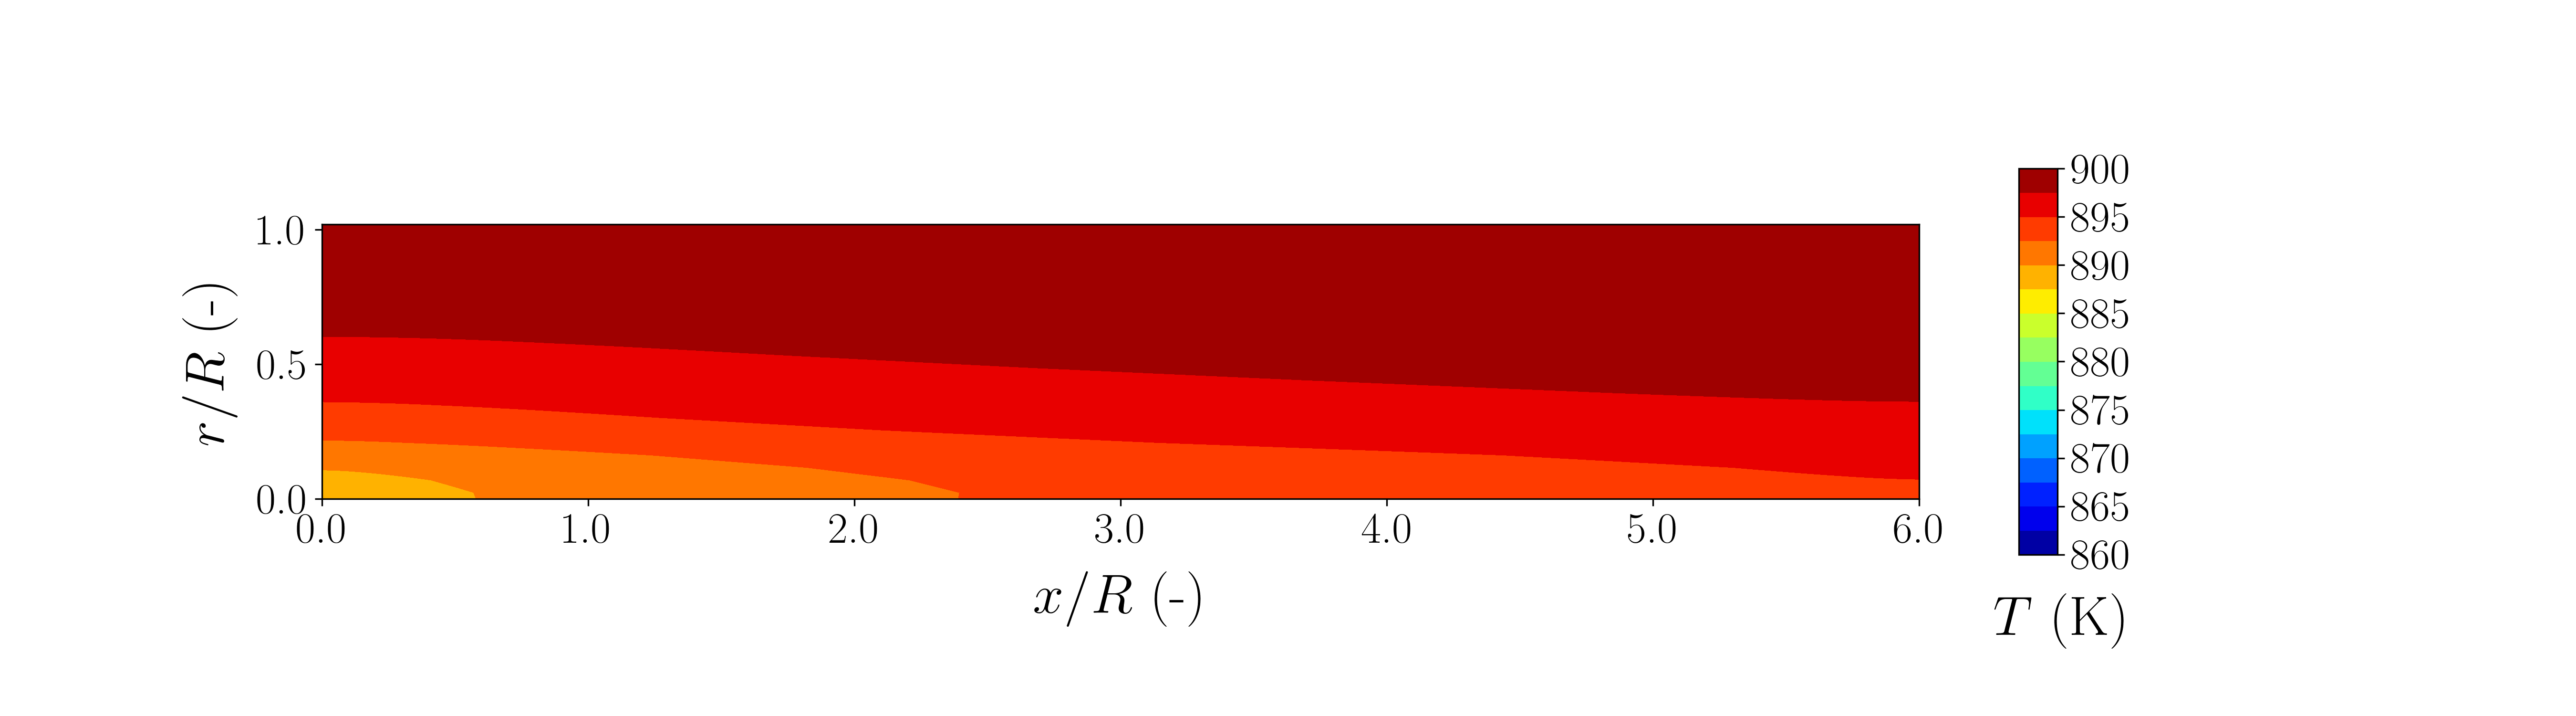
\includegraphics[width=190mm]{results/5/40C_60T/GEN30-TFIELD.png}
%\caption{\label{fig:5R4060G30-TField} Strategy I - Temperature field distribution - 30$^{\rm{th}}$ generation ($w_{\rm{CH_4}} = 0.4, w_T = 0.6$, $T_{\rm{in}}$ = 900 K, $u_{\rm{in}}$ = 0.15 m s$^{-1}$, $SC$ = 2.0)}
%\end{figure}
%
%
%\begin{figure}[h!]
%\centering
%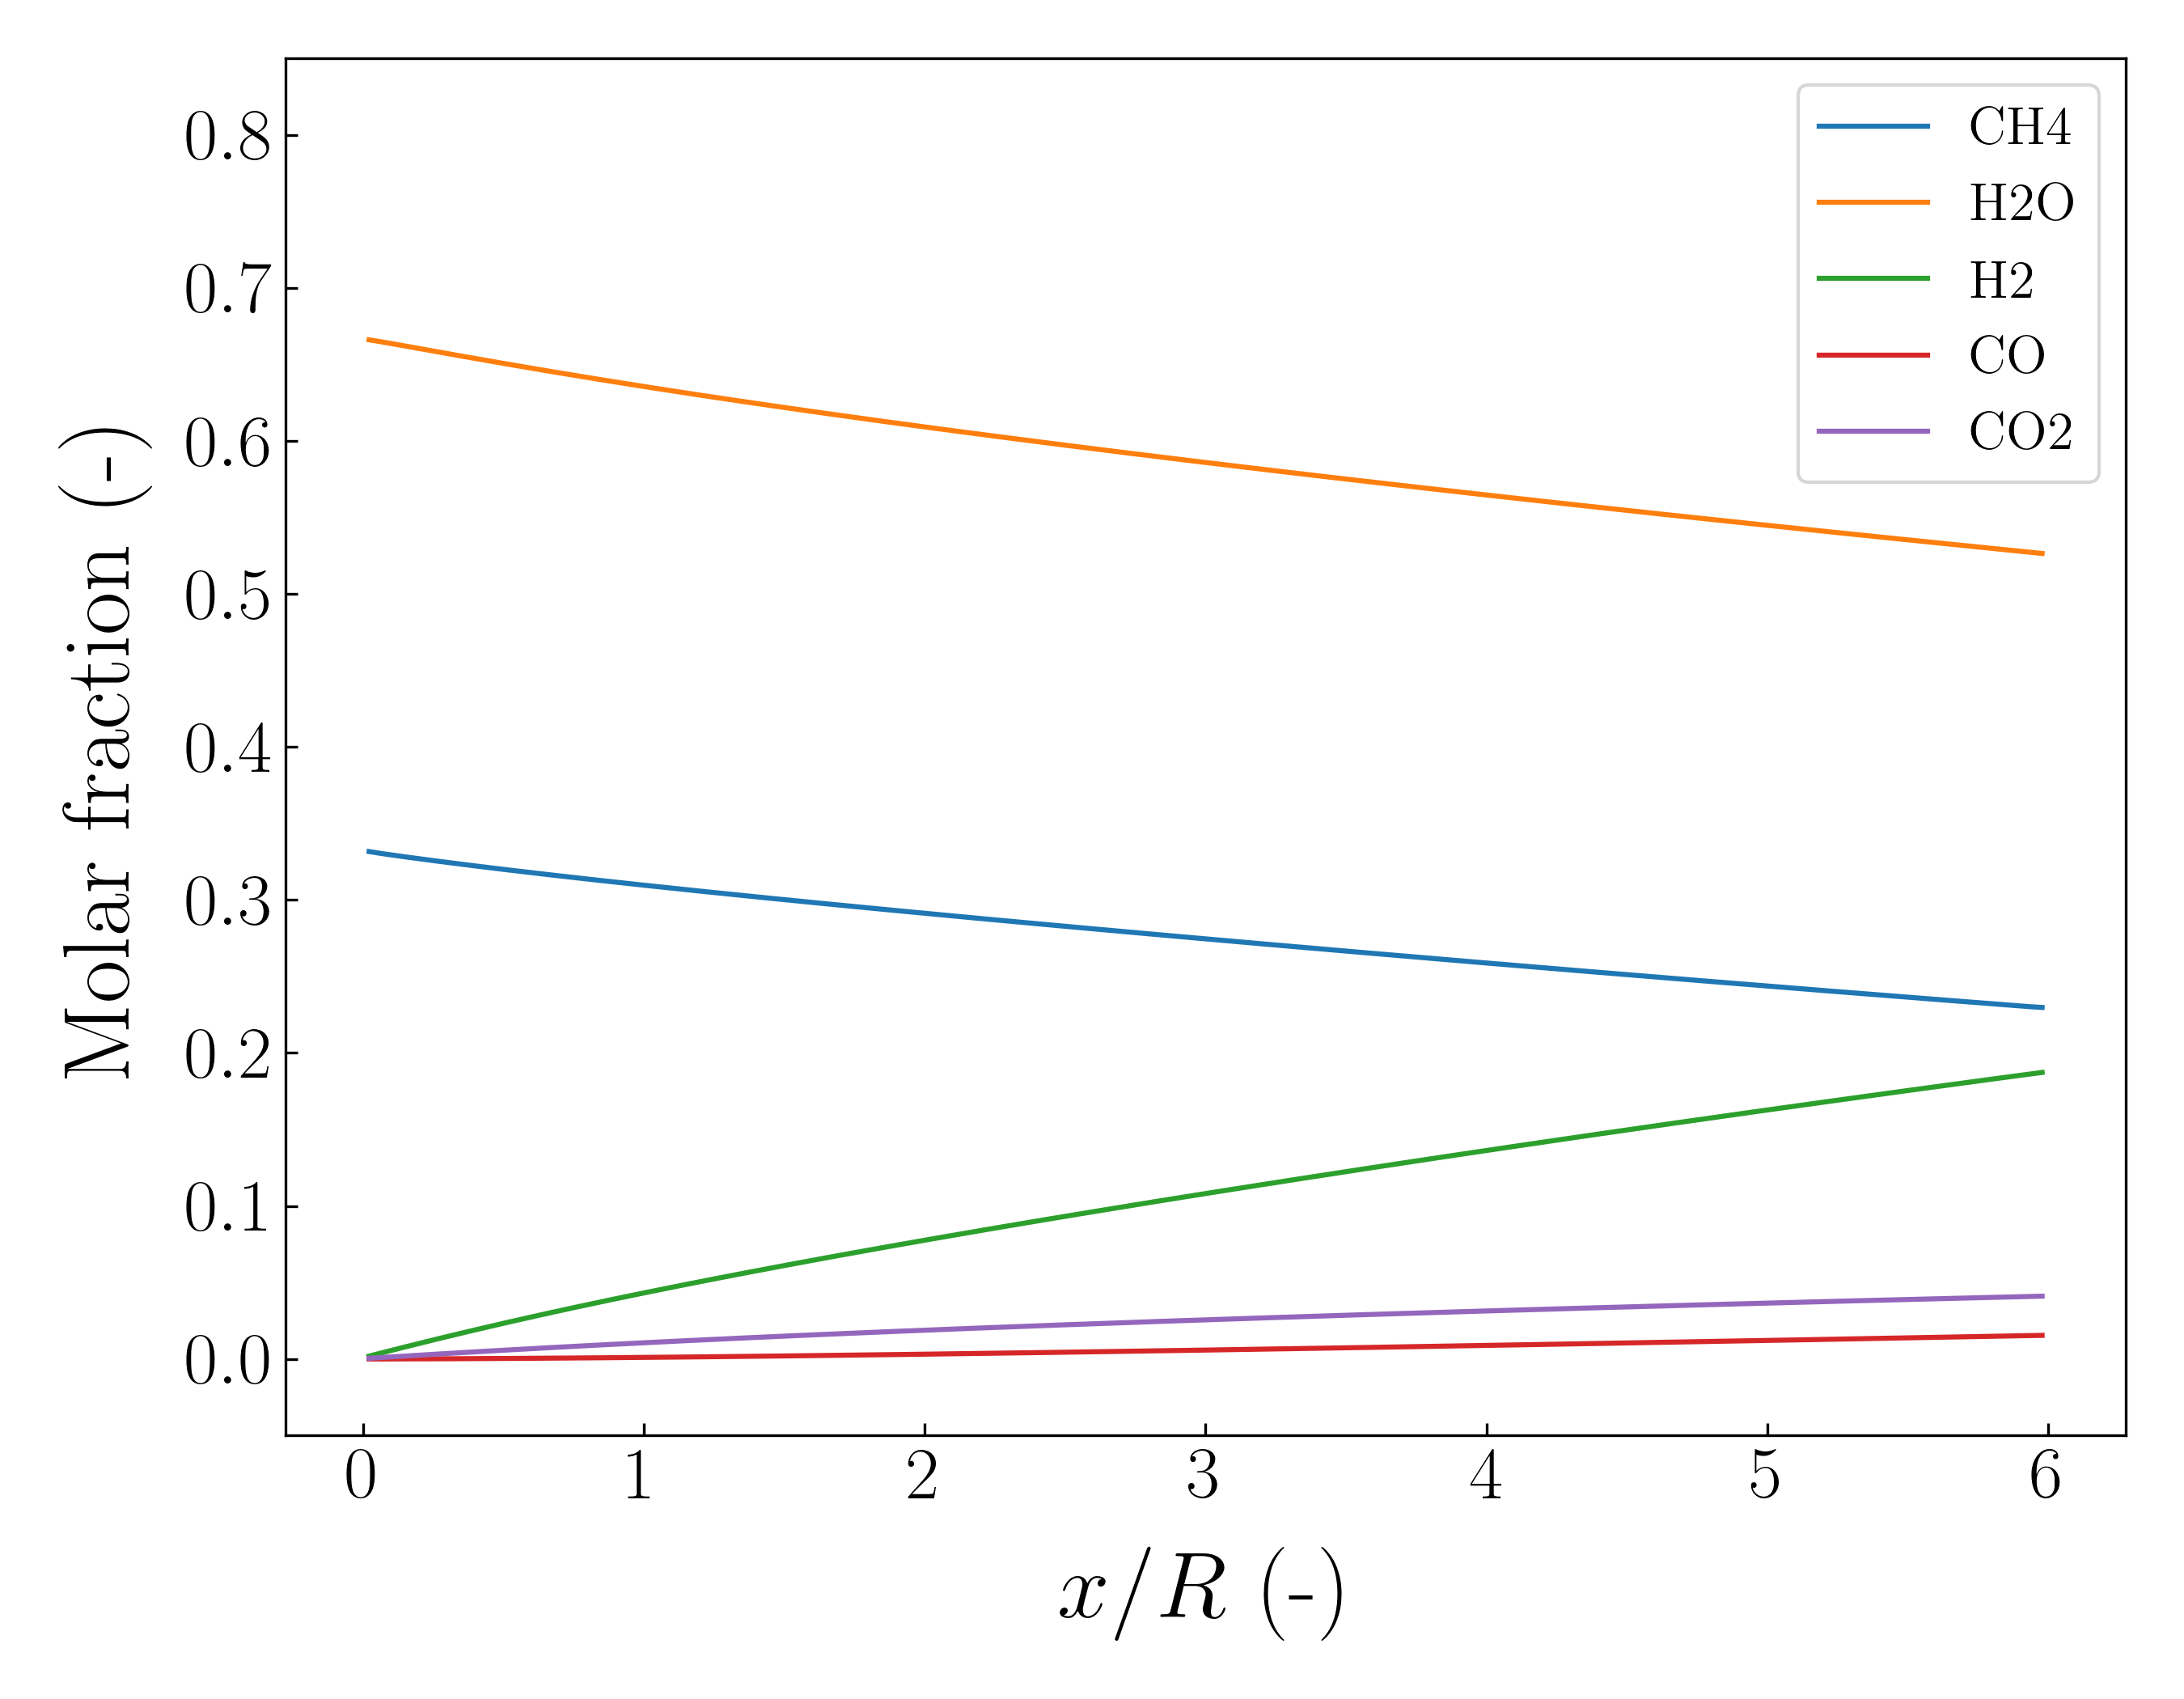
\includegraphics[width=80mm]{results/5/40C_60T/GEN1-AVG.png}
%\caption{\label{fig:5R4060G1-avg} Strategy I - Radius-averaged molar fractions - 1$^{\rm{st}}$ generation ($w_{\rm{CH_4}} = 0.4, w_T = 0.6$, $T_{\rm{in}}$ = 900 K, $u_{\rm{in}}$ = 0.15 m s$^{-1}$, $SC$ = 2.0)}
%\end{figure}
%
%\begin{figure}[h!]
%\centering
%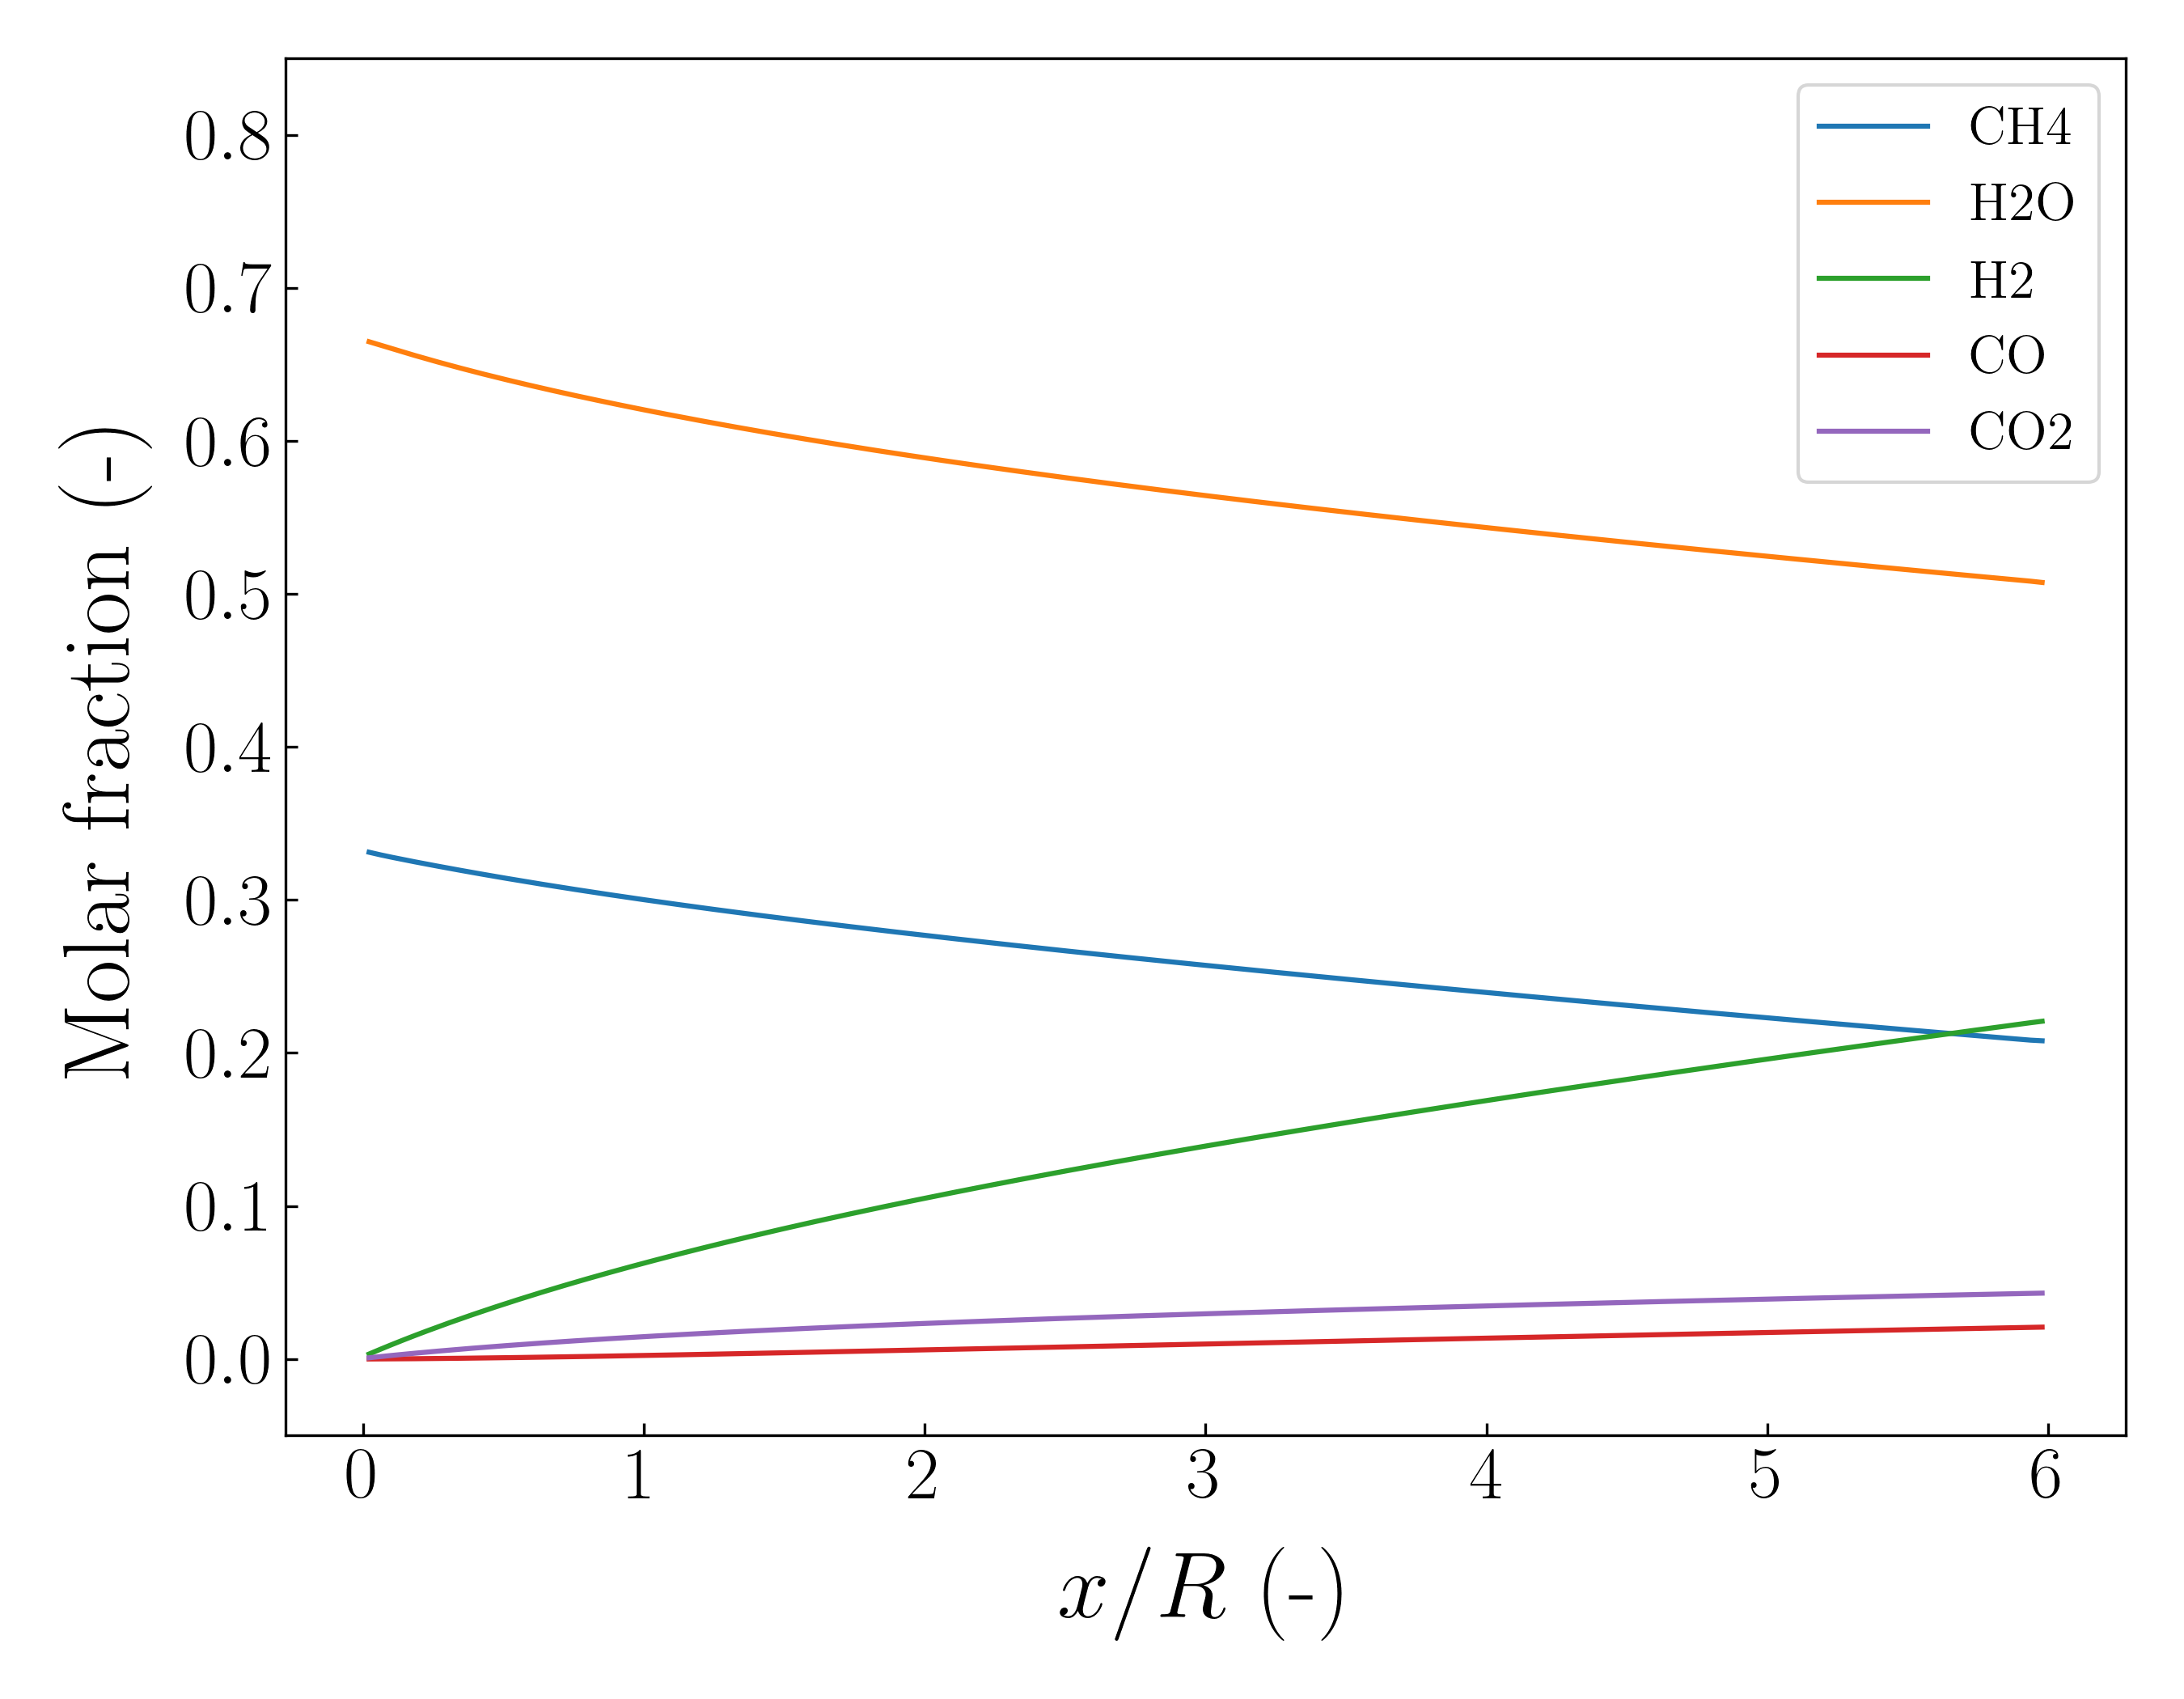
\includegraphics[width=80mm]{results/5/40C_60T/GEN15-AVG.png}
%\caption{\label{fig:5R4060G15-avg} Strategy I - Radius-averaged molar fractions - 15$^{\rm{th}}$ generation ($w_{\rm{CH_4}} = 0.4, w_T = 0.6$, $T_{\rm{in}}$ = 900 K, $u_{\rm{in}}$ = 0.15 m s$^{-1}$, $SC$ = 2.0)}
%\end{figure}
%
%\begin{figure}[h!]
%\centering
%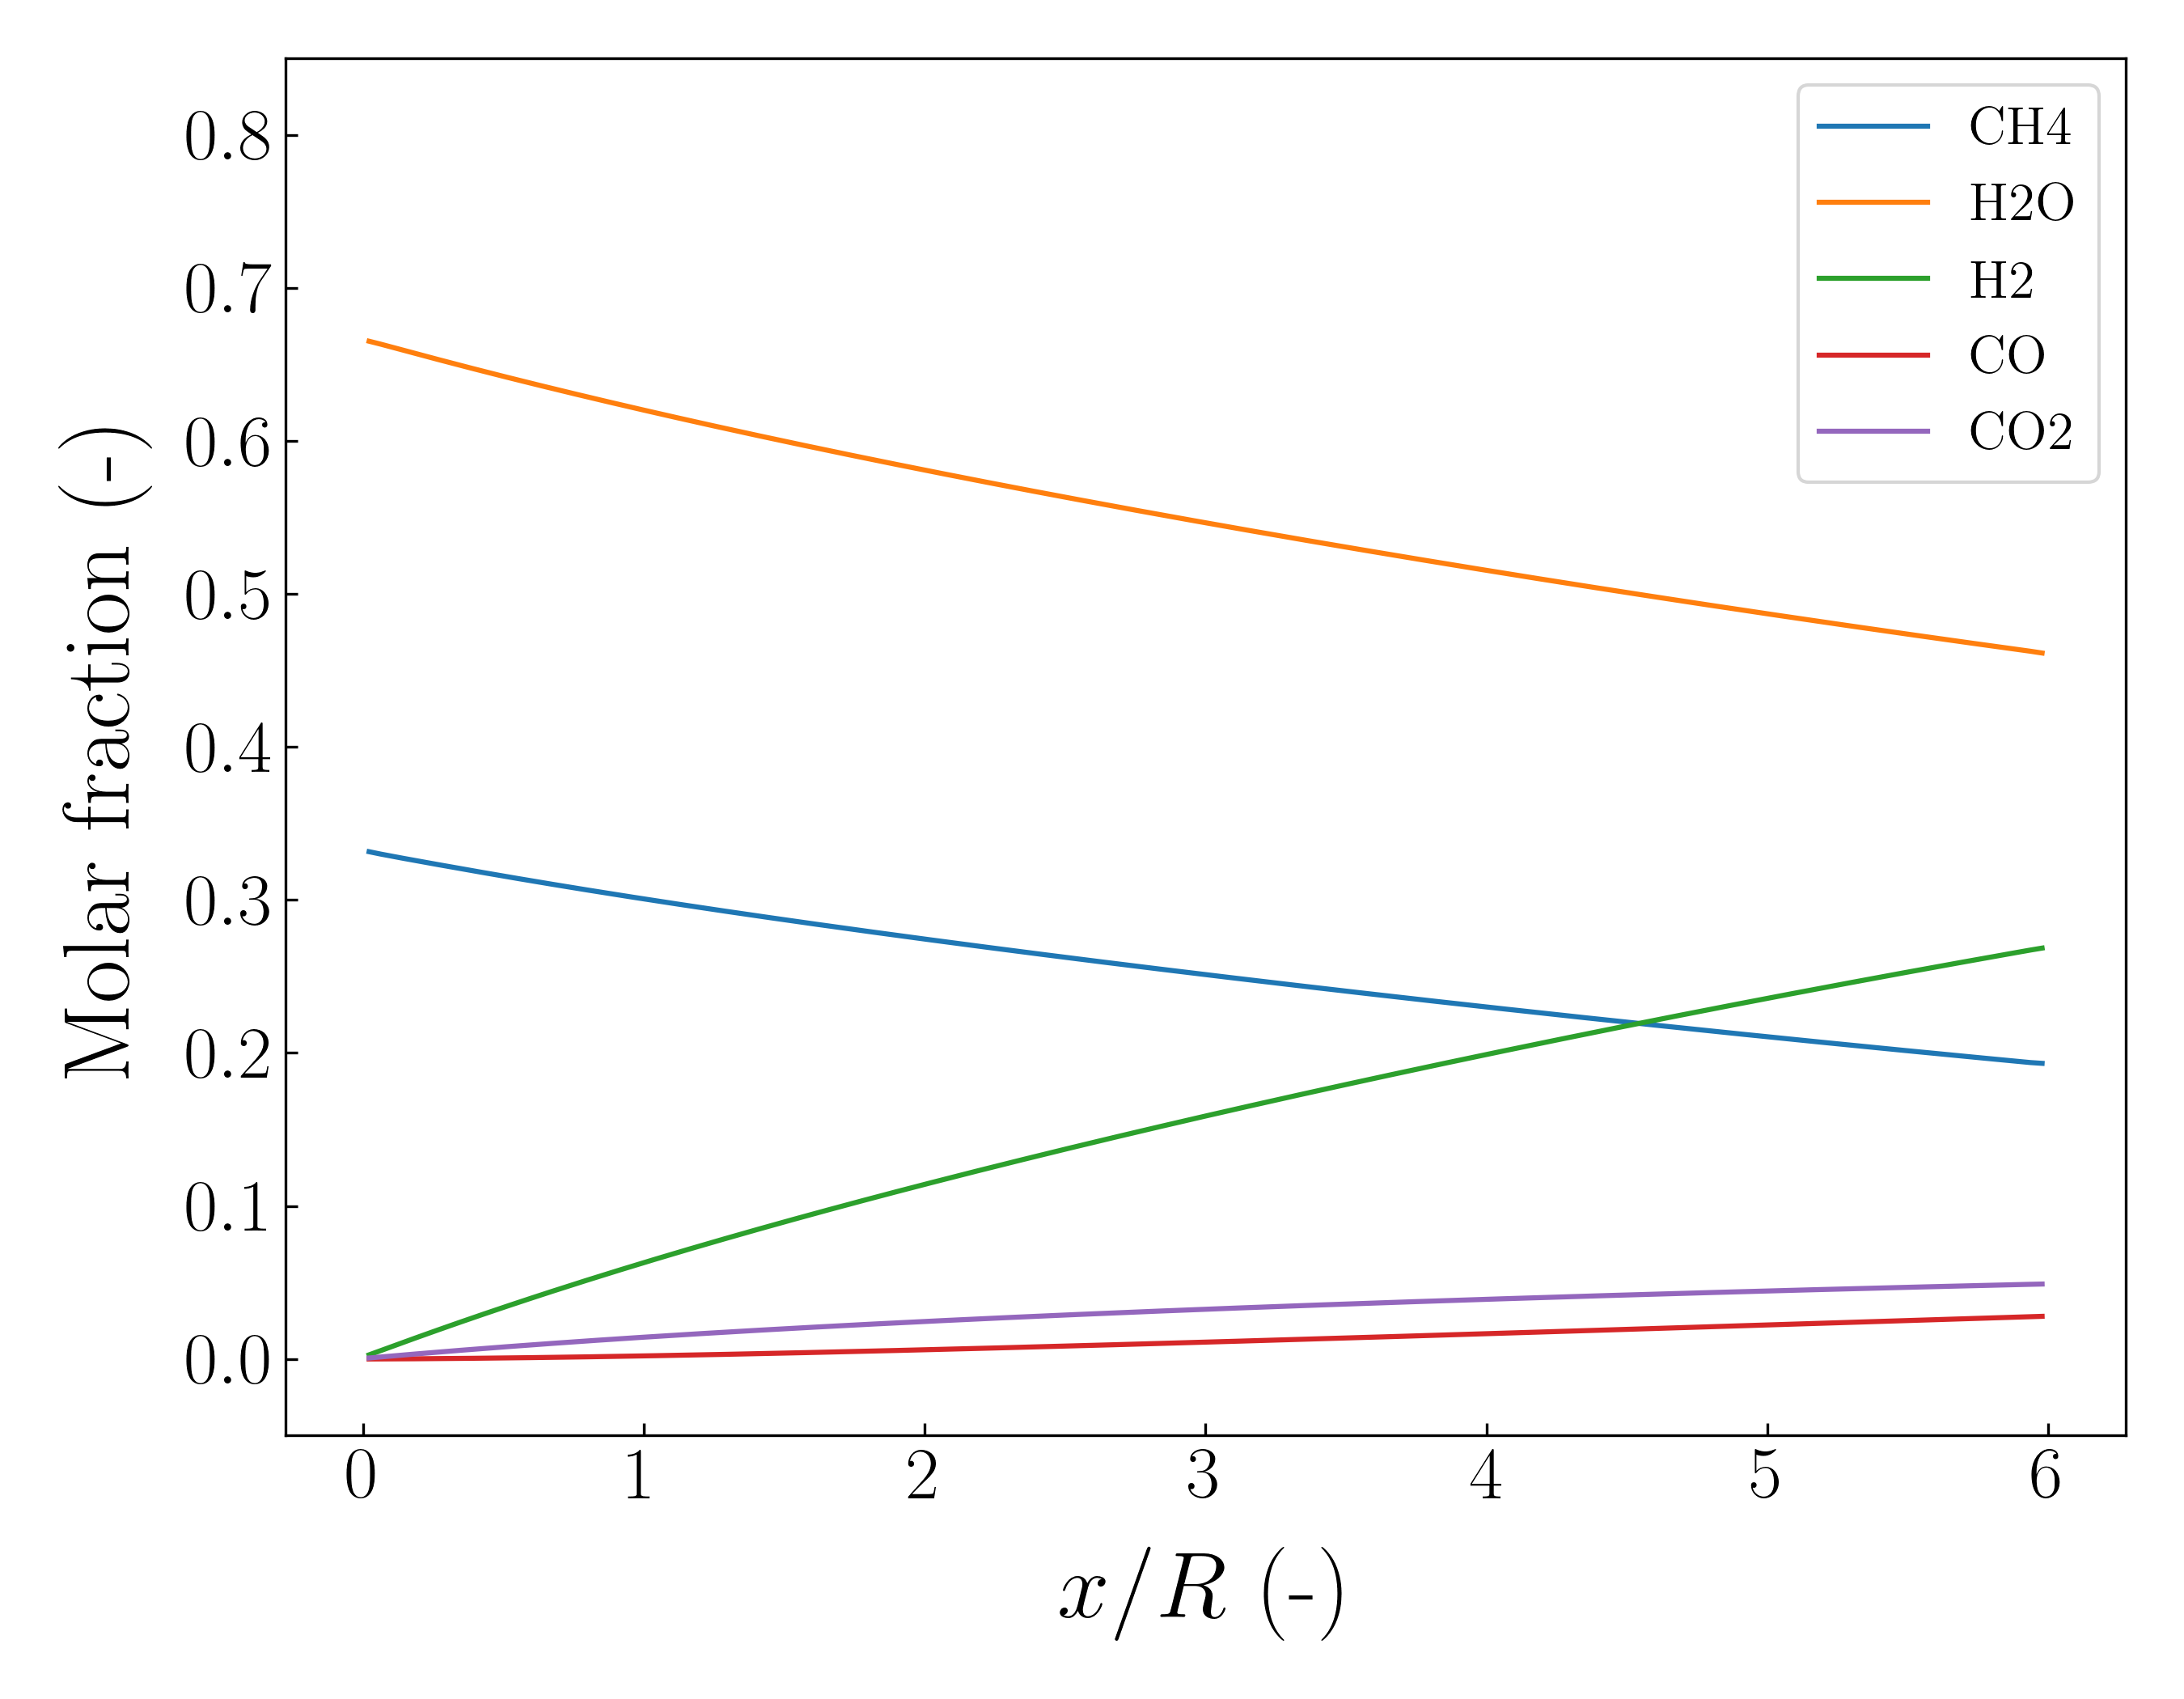
\includegraphics[width=80mm]{results/5/40C_60T/GEN30-AVG.png}
%\caption{\label{fig:5R4060G30-avg} Strategy I - Radius-averaged molar fractions -  30$^{\rm{th}}$ generation ($w_{\rm{CH_4}} = 0.4, w_T = 0.6$, $T_{\rm{in}}$ = 900 K, $u_{\rm{in}}$ = 0.15 m s$^{-1}$, $SC$ = 2.0)}
%\end{figure}
%
%\begin{figure}[h!]
%\centering
%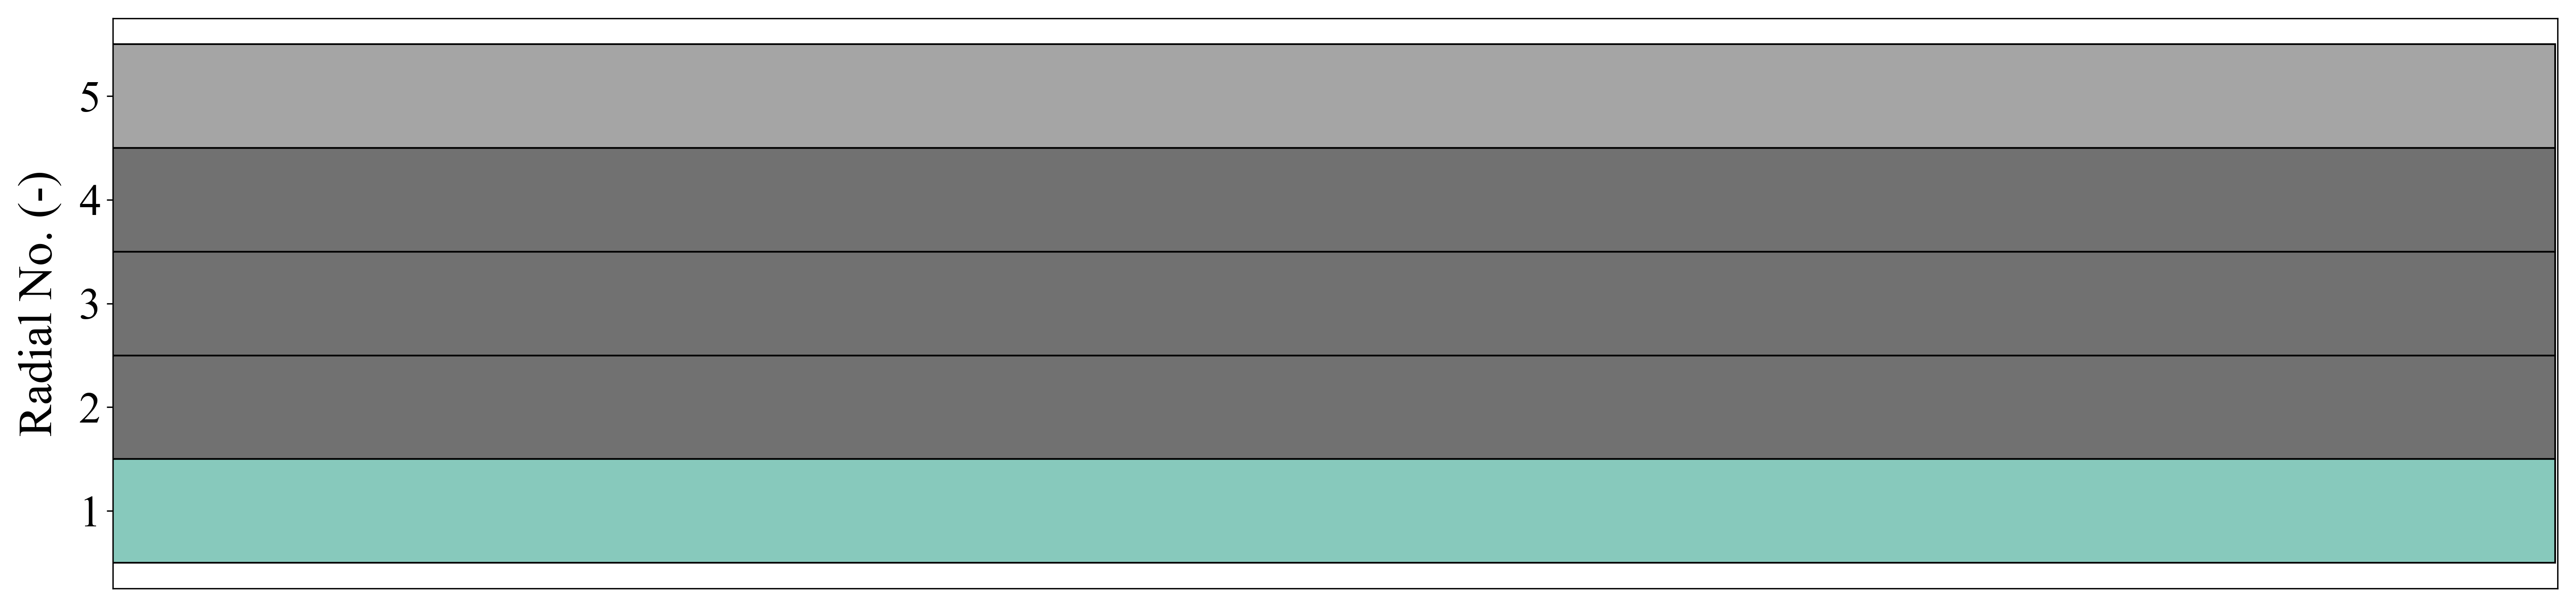
\includegraphics[width=120mm]{results/segments/5seg/40C60T/seg.png}
%\caption{\label{fig:30L6040G1-TField} Strategy I - Segments distribution for 30$^{\rm{th}}$ generation ($w_{\rm{CH_4}} = 0.4, w_T = 0.6$, $T_{\rm{in}}$ = 900 K, $u_{\rm{in}}$ = 0.15 m s$^{-1}$, $SC$ = 2.0)}
%\end{figure}
%
%\begin{figure}[h!]
%\centering
%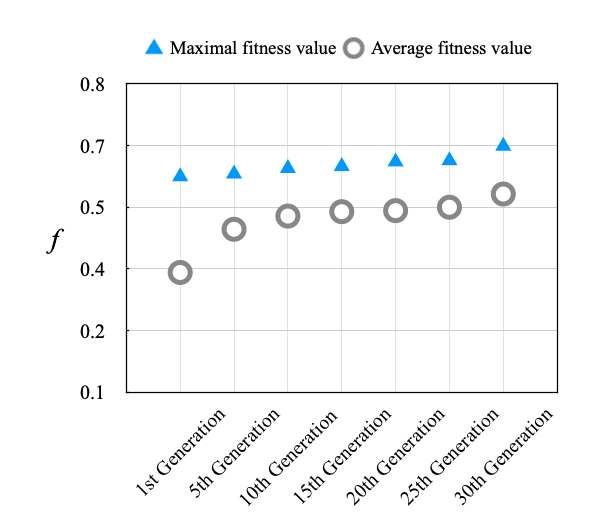
\includegraphics[width=100mm]{results/5/40C_60T.png}
%\caption{\label{fig:5R4060G-fitness} Strategy I - Fitness analysis throughout successive populations ($w_{\rm{CH_4}} = 0.4, w_T = 0.6$, $T_{\rm{in}}$ = 900 K, $u_{\rm{in}}$ = 0.15 m s$^{-1}$, $SC$ = 2.0)}
%\end{figure}
%
%
%\clearpage
%
%
%
%
%
%\paragraph{Thermal fitness 50 \%, methane conversion 50 \%} \hspace{0pt} \\
%\noindent 
%
%
%\begin{figure}[h!]
%\centering
%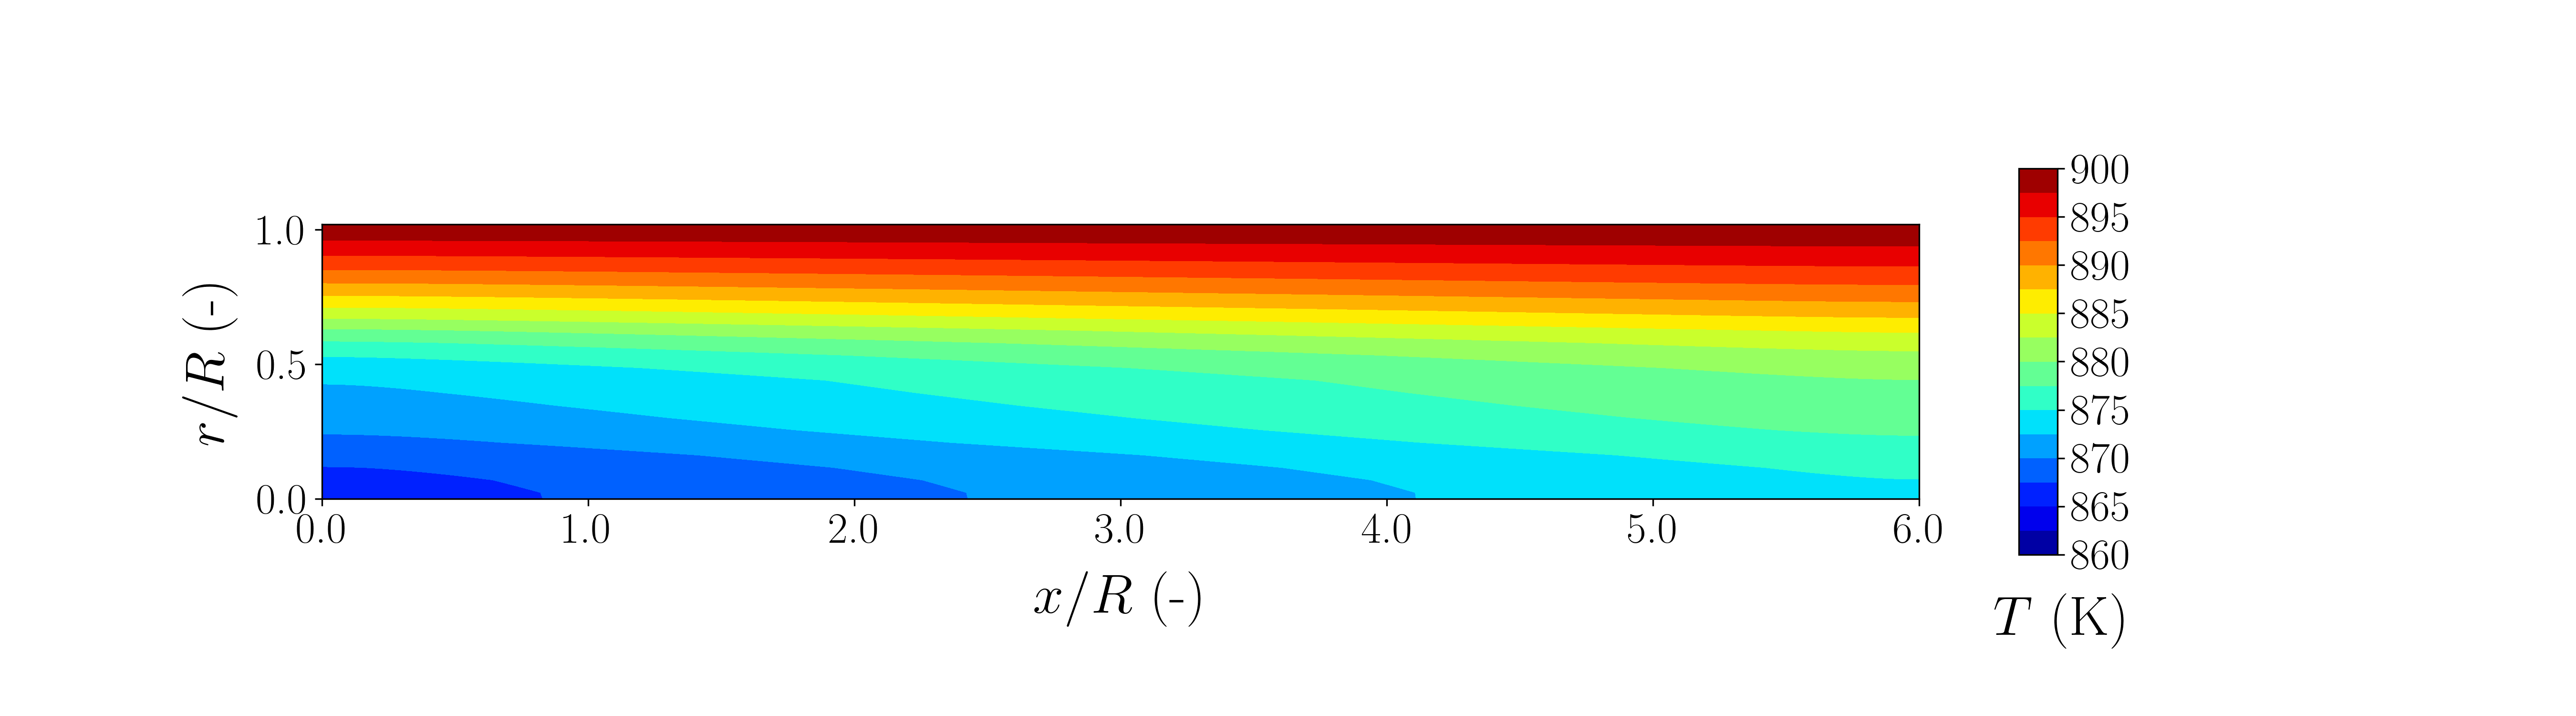
\includegraphics[width=190mm]{results/5/50C_50T/GEN1-TFIELD.png}
%\caption{\label{fig:5R5050G1-TField} Strategy I - Temperature field distribution - 1$^{\rm{st}}$ generation ($w_{\rm{CH_4}} = 0.5, w_T = 0.5$, $T_{\rm{in}}$ = 900 K, $u_{\rm{in}}$ = 0.15 m s$^{-1}$, $SC$ = 2.0)}
%\end{figure}
%
%\begin{figure}[h!]
%\centering
%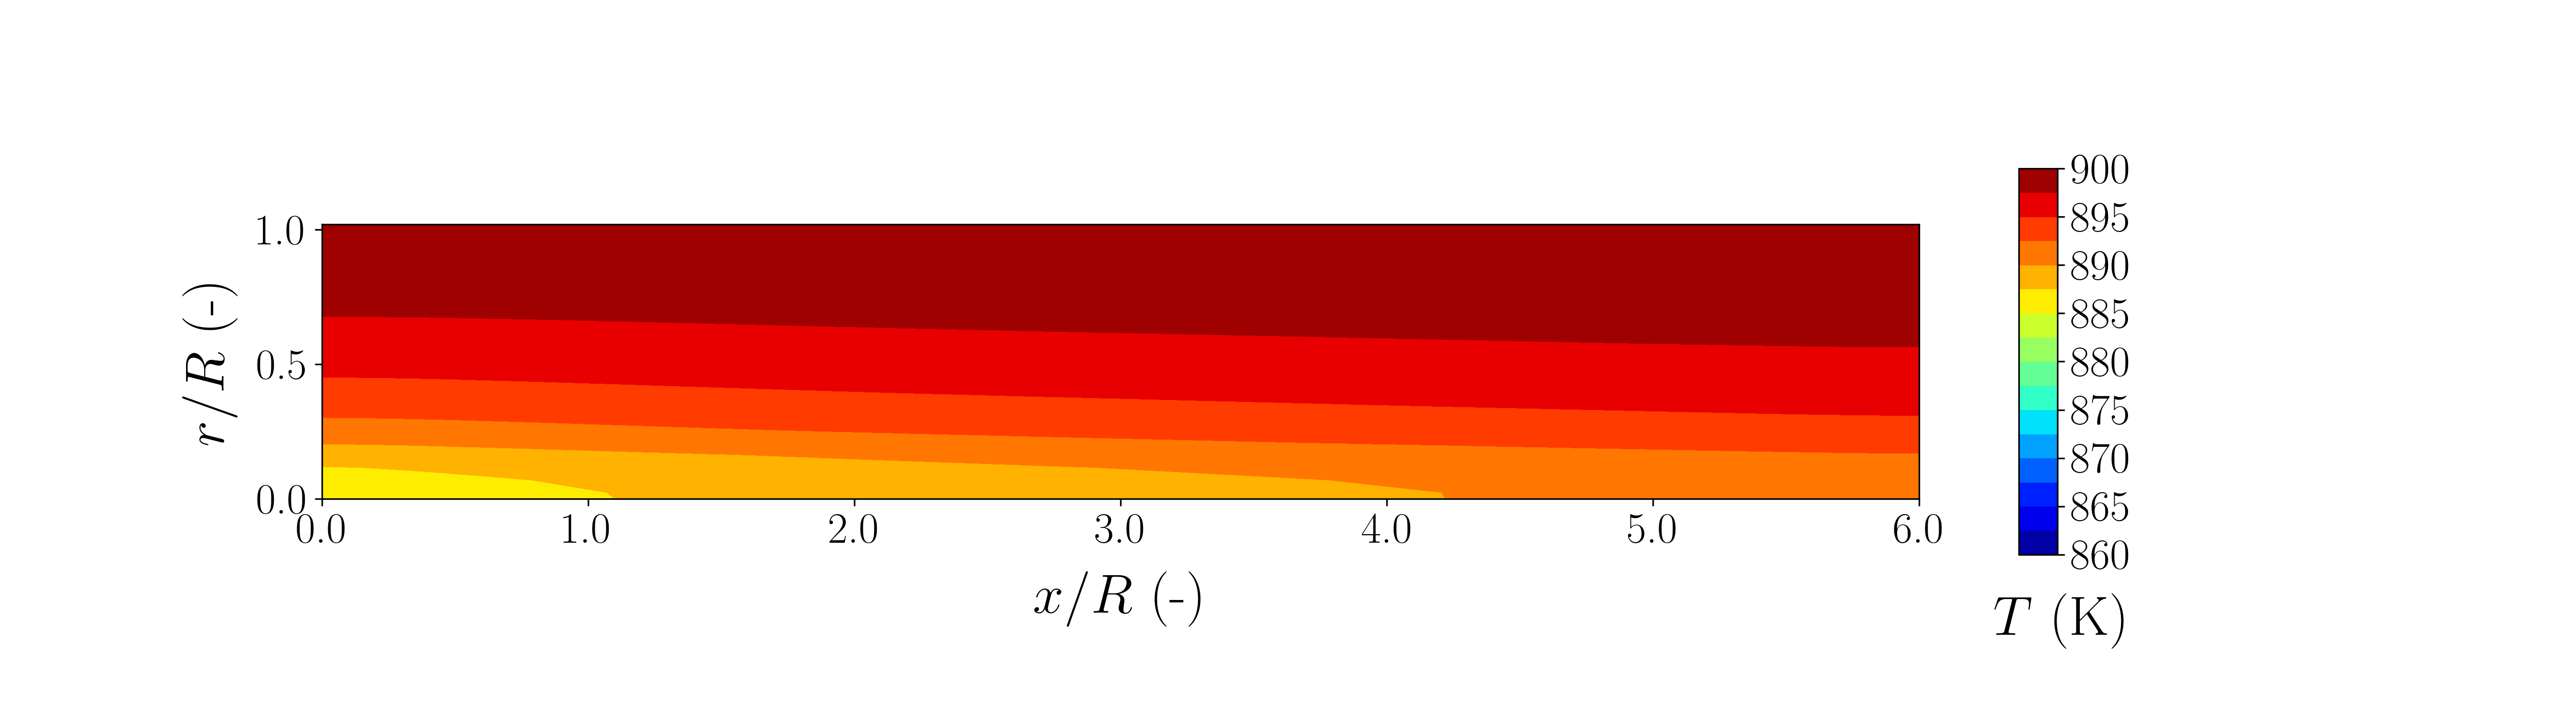
\includegraphics[width=190mm]{results/5/50C_50T/GEN15-TFIELD.png}
%\caption{\label{fig:5R5050G15-TField} Strategy I - Temperature field distribution - 15$^{\rm{th}}$ generation ($w_{\rm{CH_4}} = 0.5, w_T = 0.5$, $T_{\rm{in}}$ = 900 K, $u_{\rm{in}}$ = 0.15 m s$^{-1}$, $SC$ = 2.0)}
%\end{figure}
%
%\begin{figure}[h!]
%\centering
%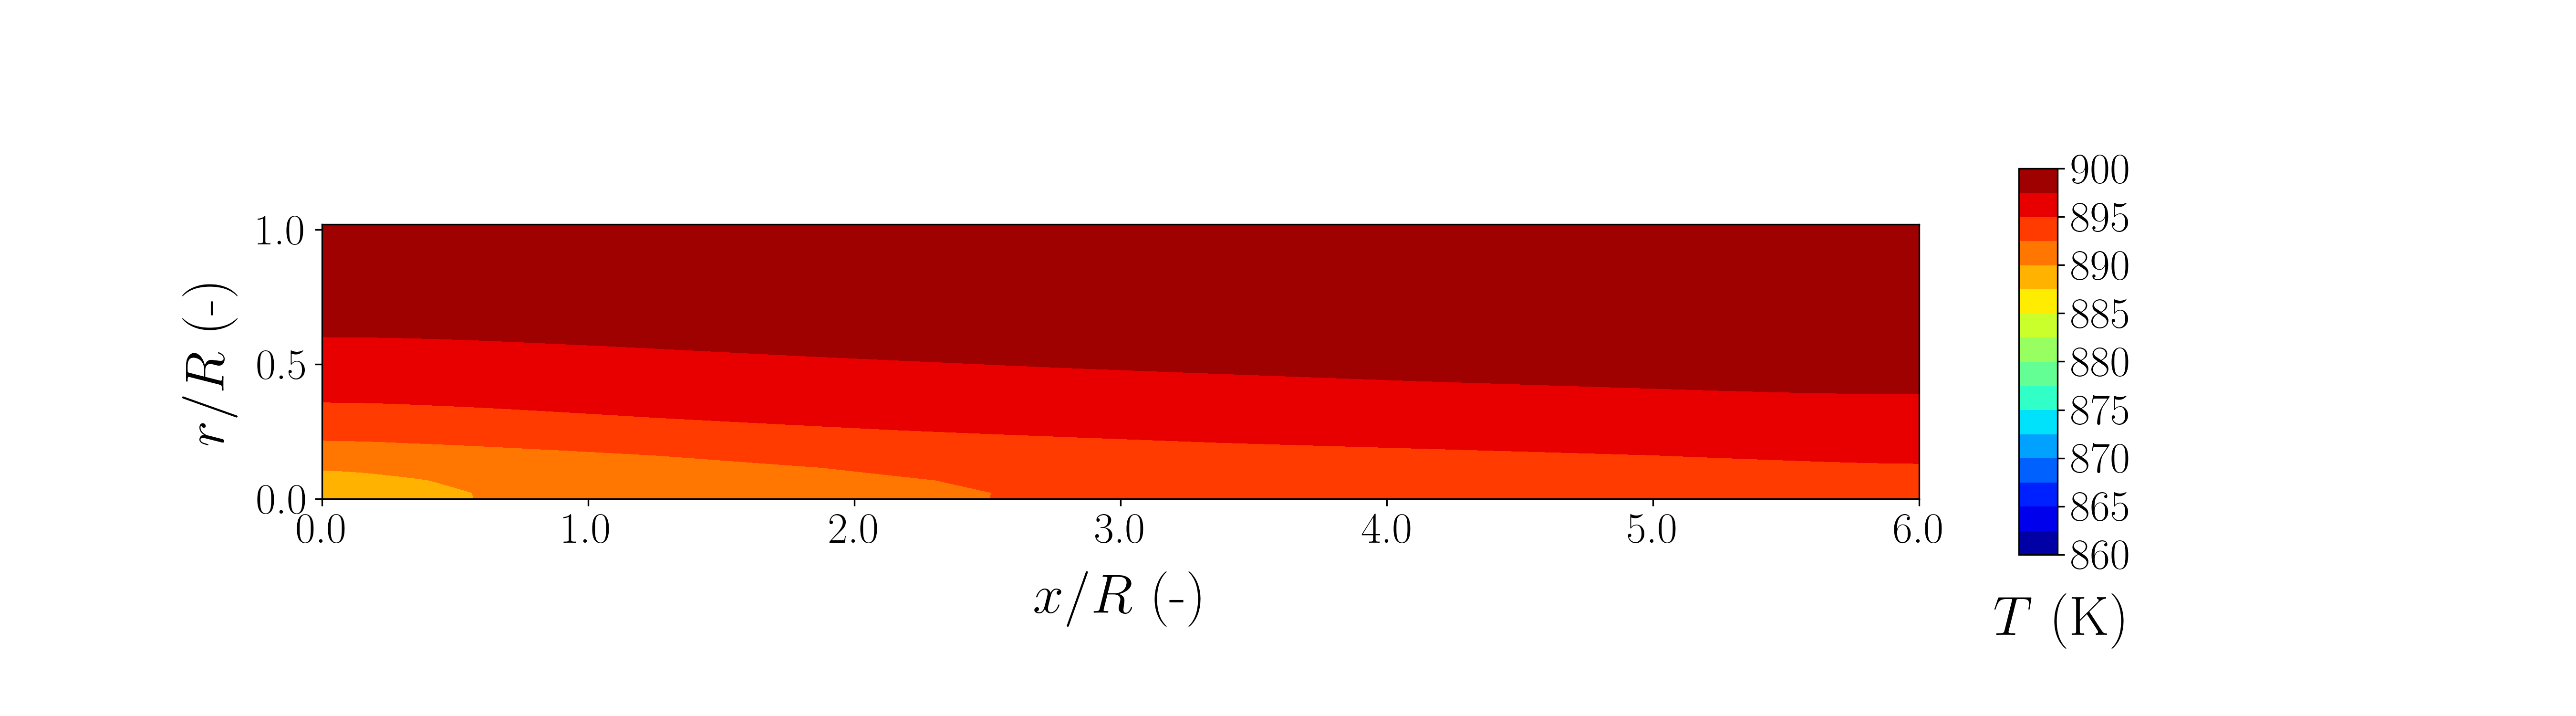
\includegraphics[width=190mm]{results/5/50C_50T/GEN30-TFIELD.png}
%\caption{\label{fig:5R5050G30-TField} Strategy I - Temperature field distribution - 30$^{\rm{th}}$ generation ($w_{\rm{CH_4}} = 0.5, w_T = 0.5$, $T_{\rm{in}}$ = 900 K, $u_{\rm{in}}$ = 0.15 m s$^{-1}$, $SC$ = 2.0)}
%\end{figure}
%
%
%\begin{figure}[h!]
%\centering
%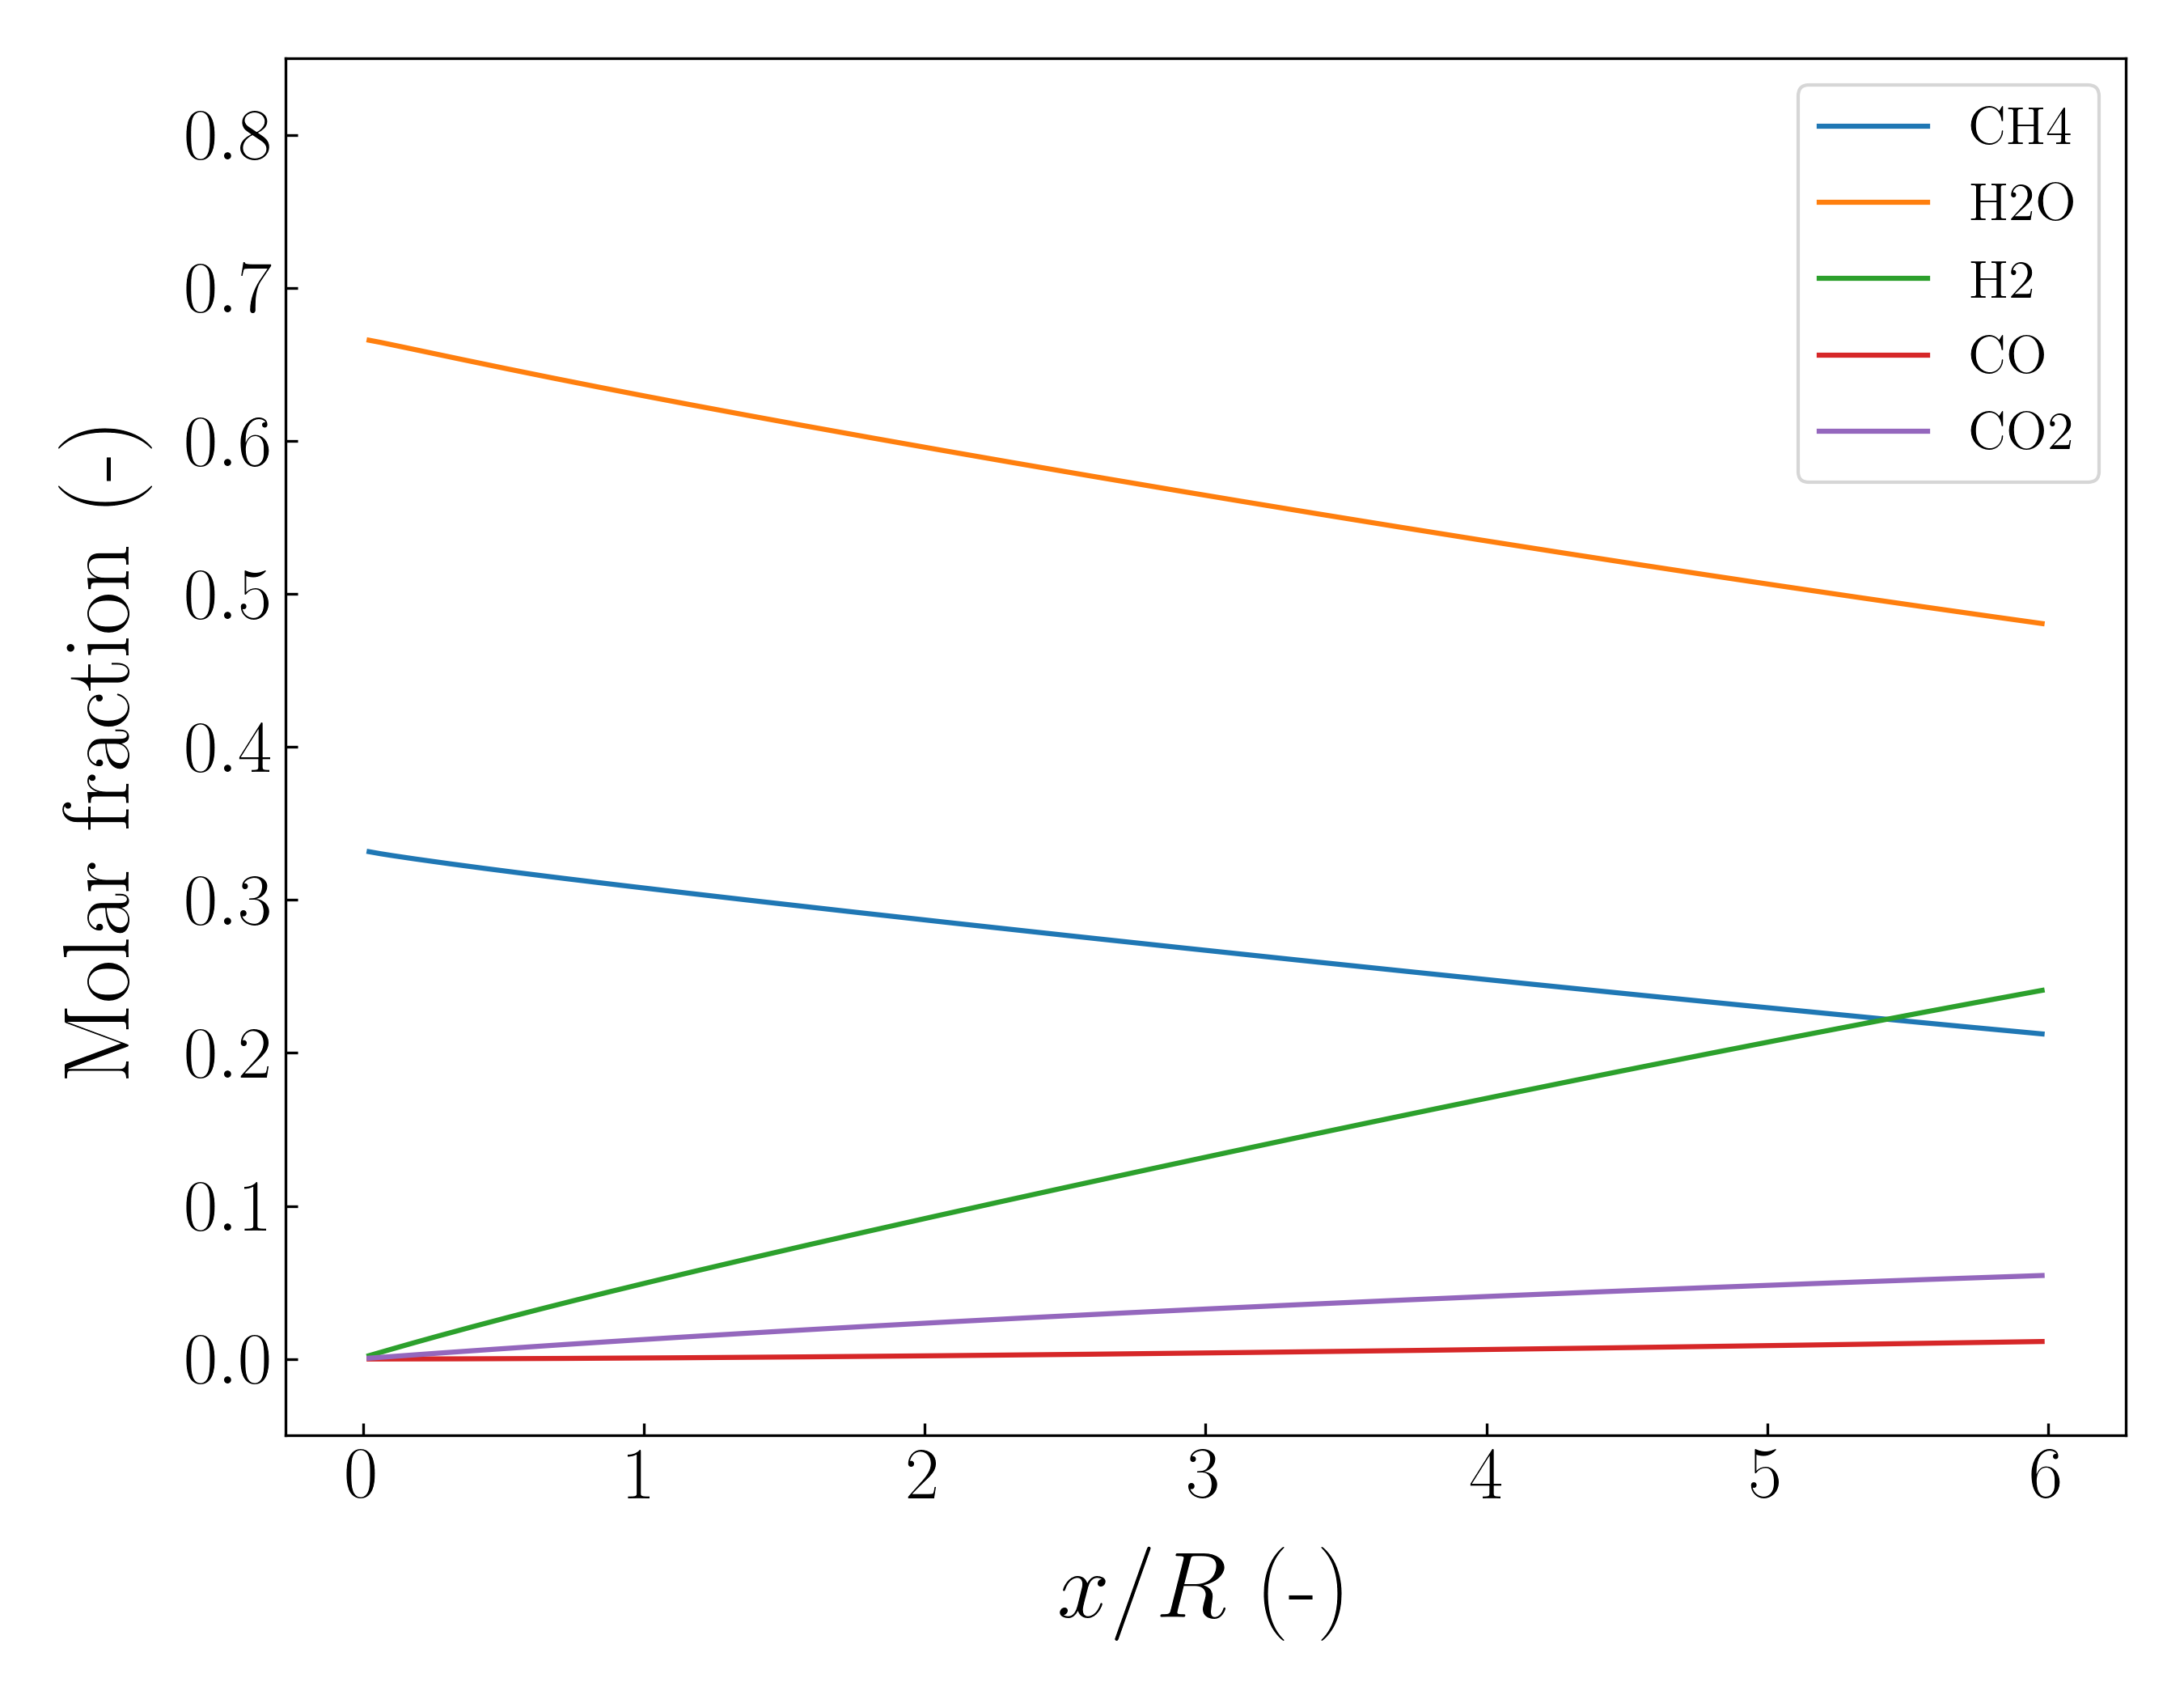
\includegraphics[width=80mm]{results/5/50C_50T/GEN1-AVG.png}
%\caption{\label{fig:5R5050G1-avg} Strategy I - Radius-averaged molar fractions - 1$^{\rm{st}}$ generation ($w_{\rm{CH_4}} = 0.5, w_T = 0.5$, $T_{\rm{in}}$ = 900 K, $u_{\rm{in}}$ = 0.15 m s$^{-1}$, $SC$ = 2.0)}
%\end{figure}
%
%\begin{figure}[h!]
%\centering
%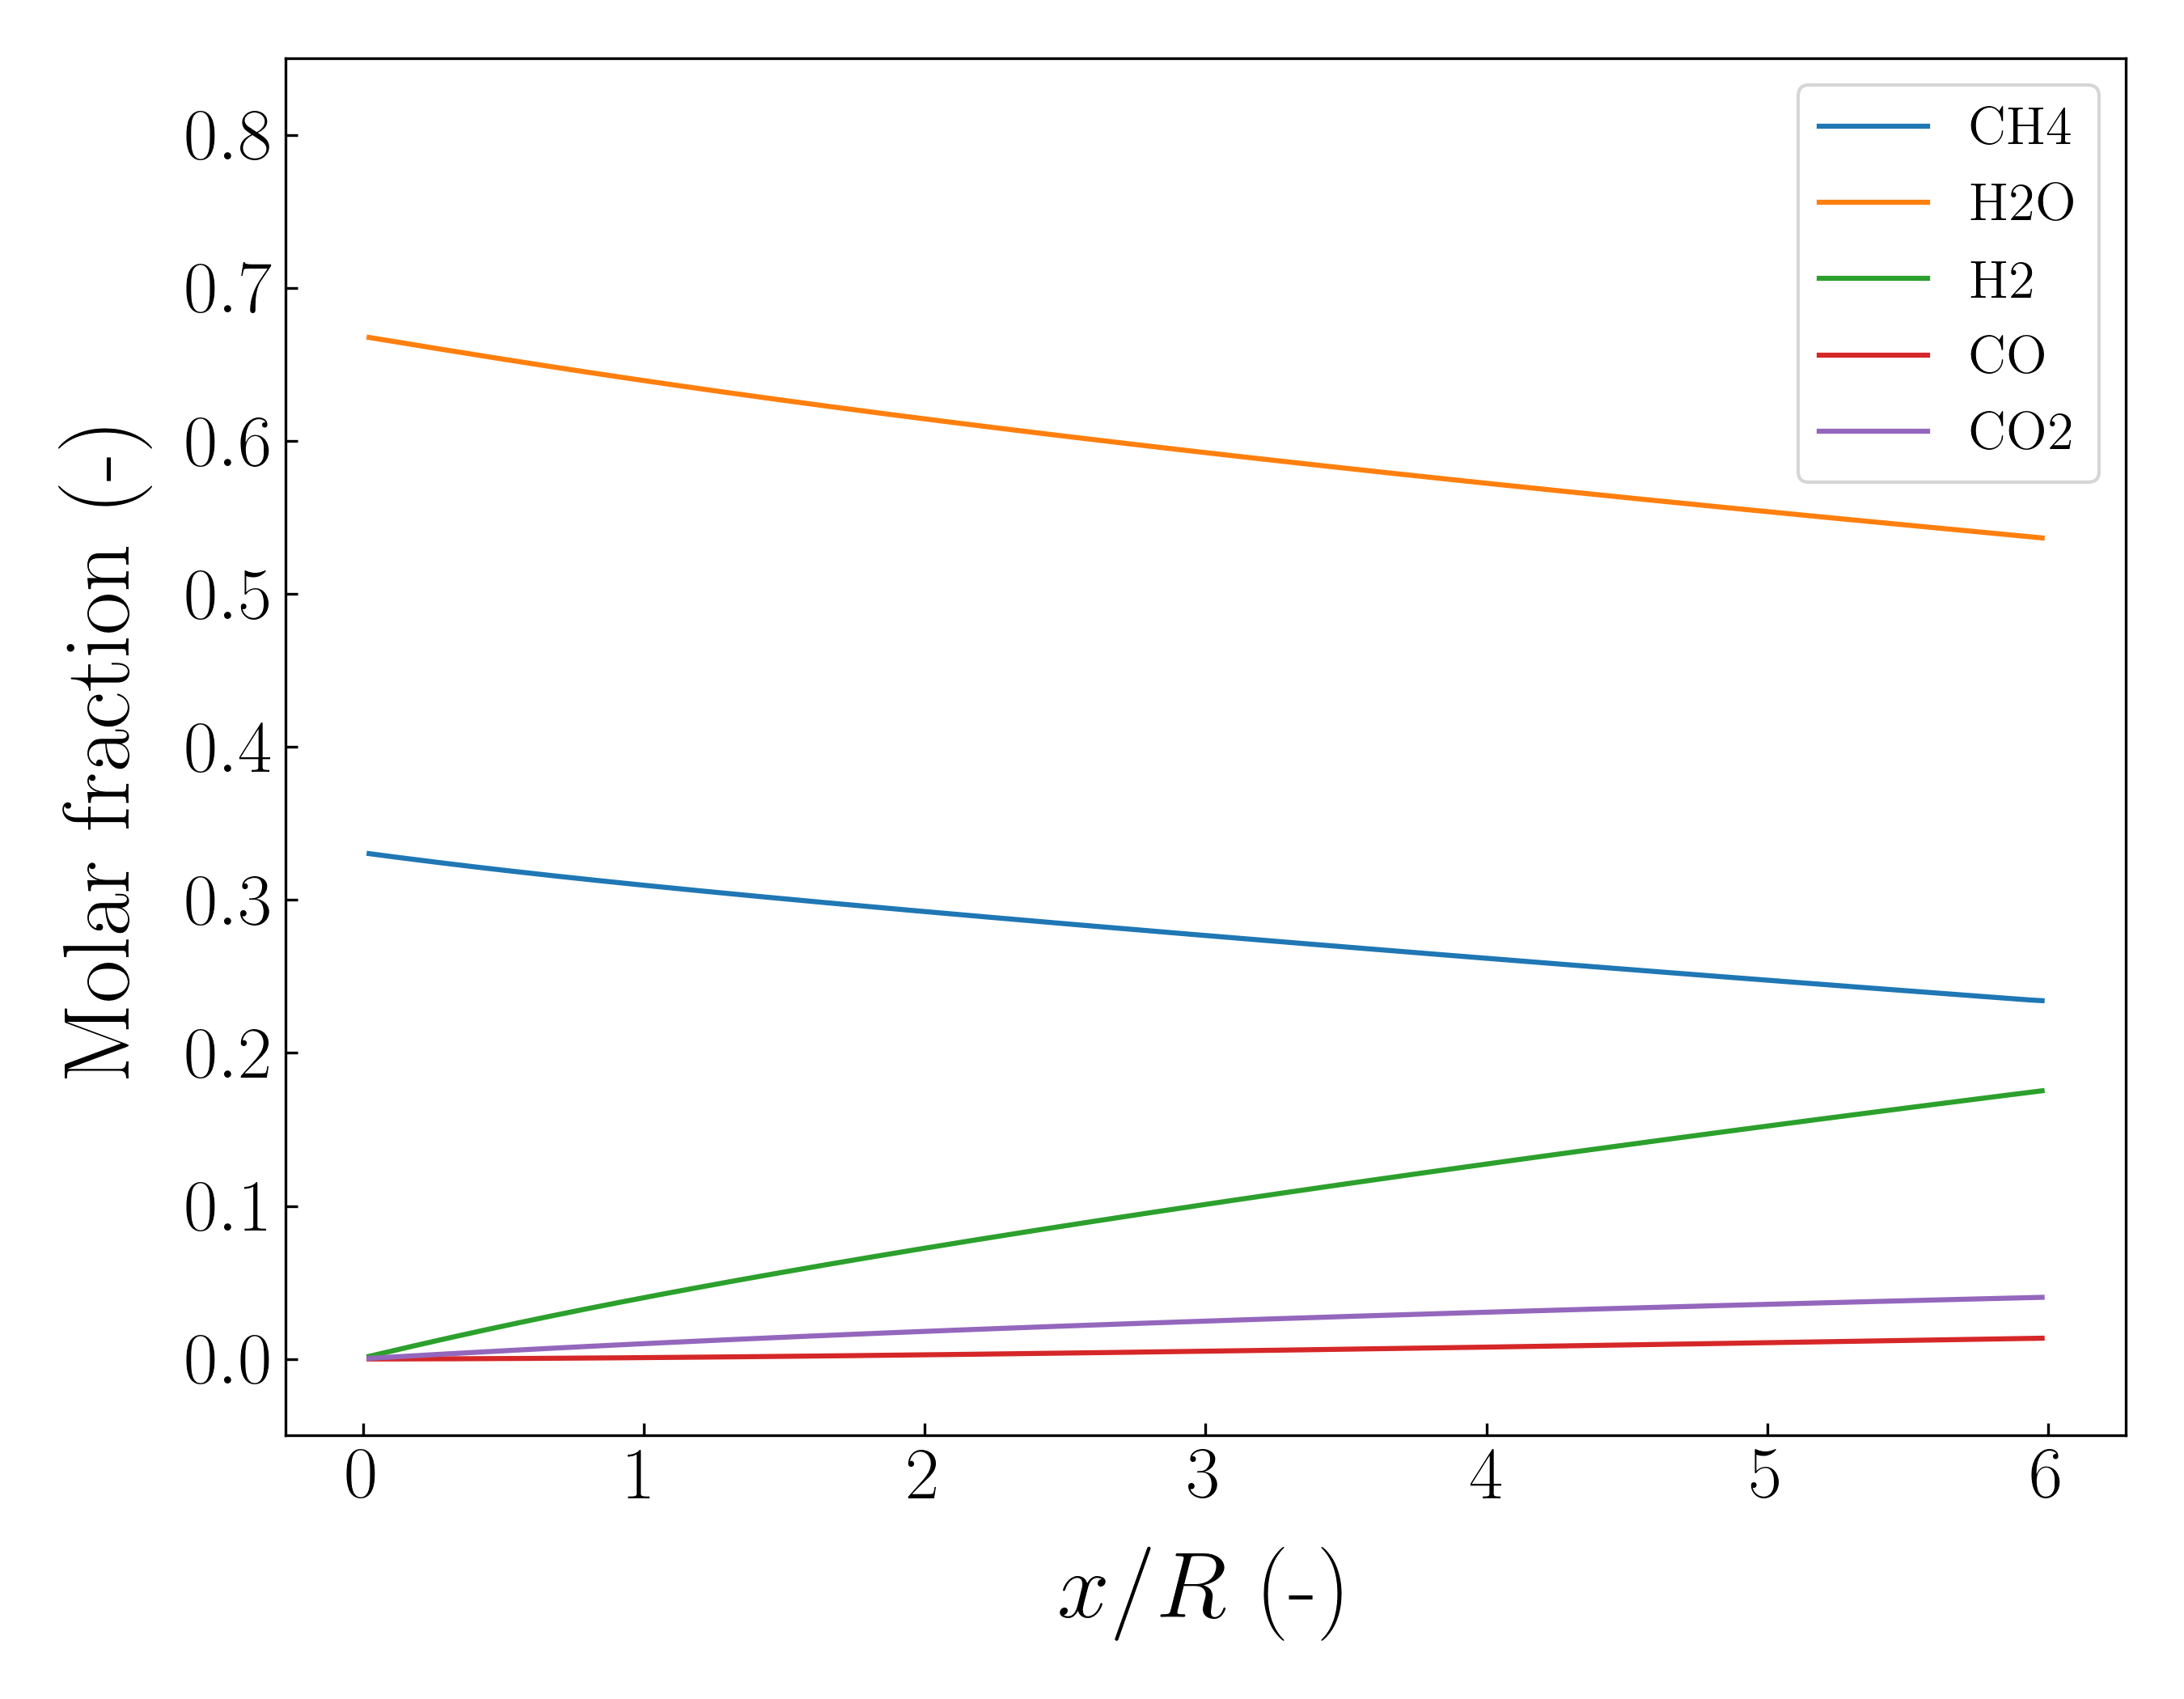
\includegraphics[width=80mm]{results/5/50C_50T/GEN15-AVG.png}
%\caption{\label{fig:5R5050G15-avg} Strategy I - Radius-averaged molar fractions - 15$^{\rm{th}}$ generation ($w_{\rm{CH_4}} = 0.5, w_T = 0.5$, $T_{\rm{in}}$ = 900 K, $u_{\rm{in}}$ = 0.15 m s$^{-1}$, $SC$ = 2.0)}
%\end{figure}
%
%\begin{figure}[h!]
%\centering
%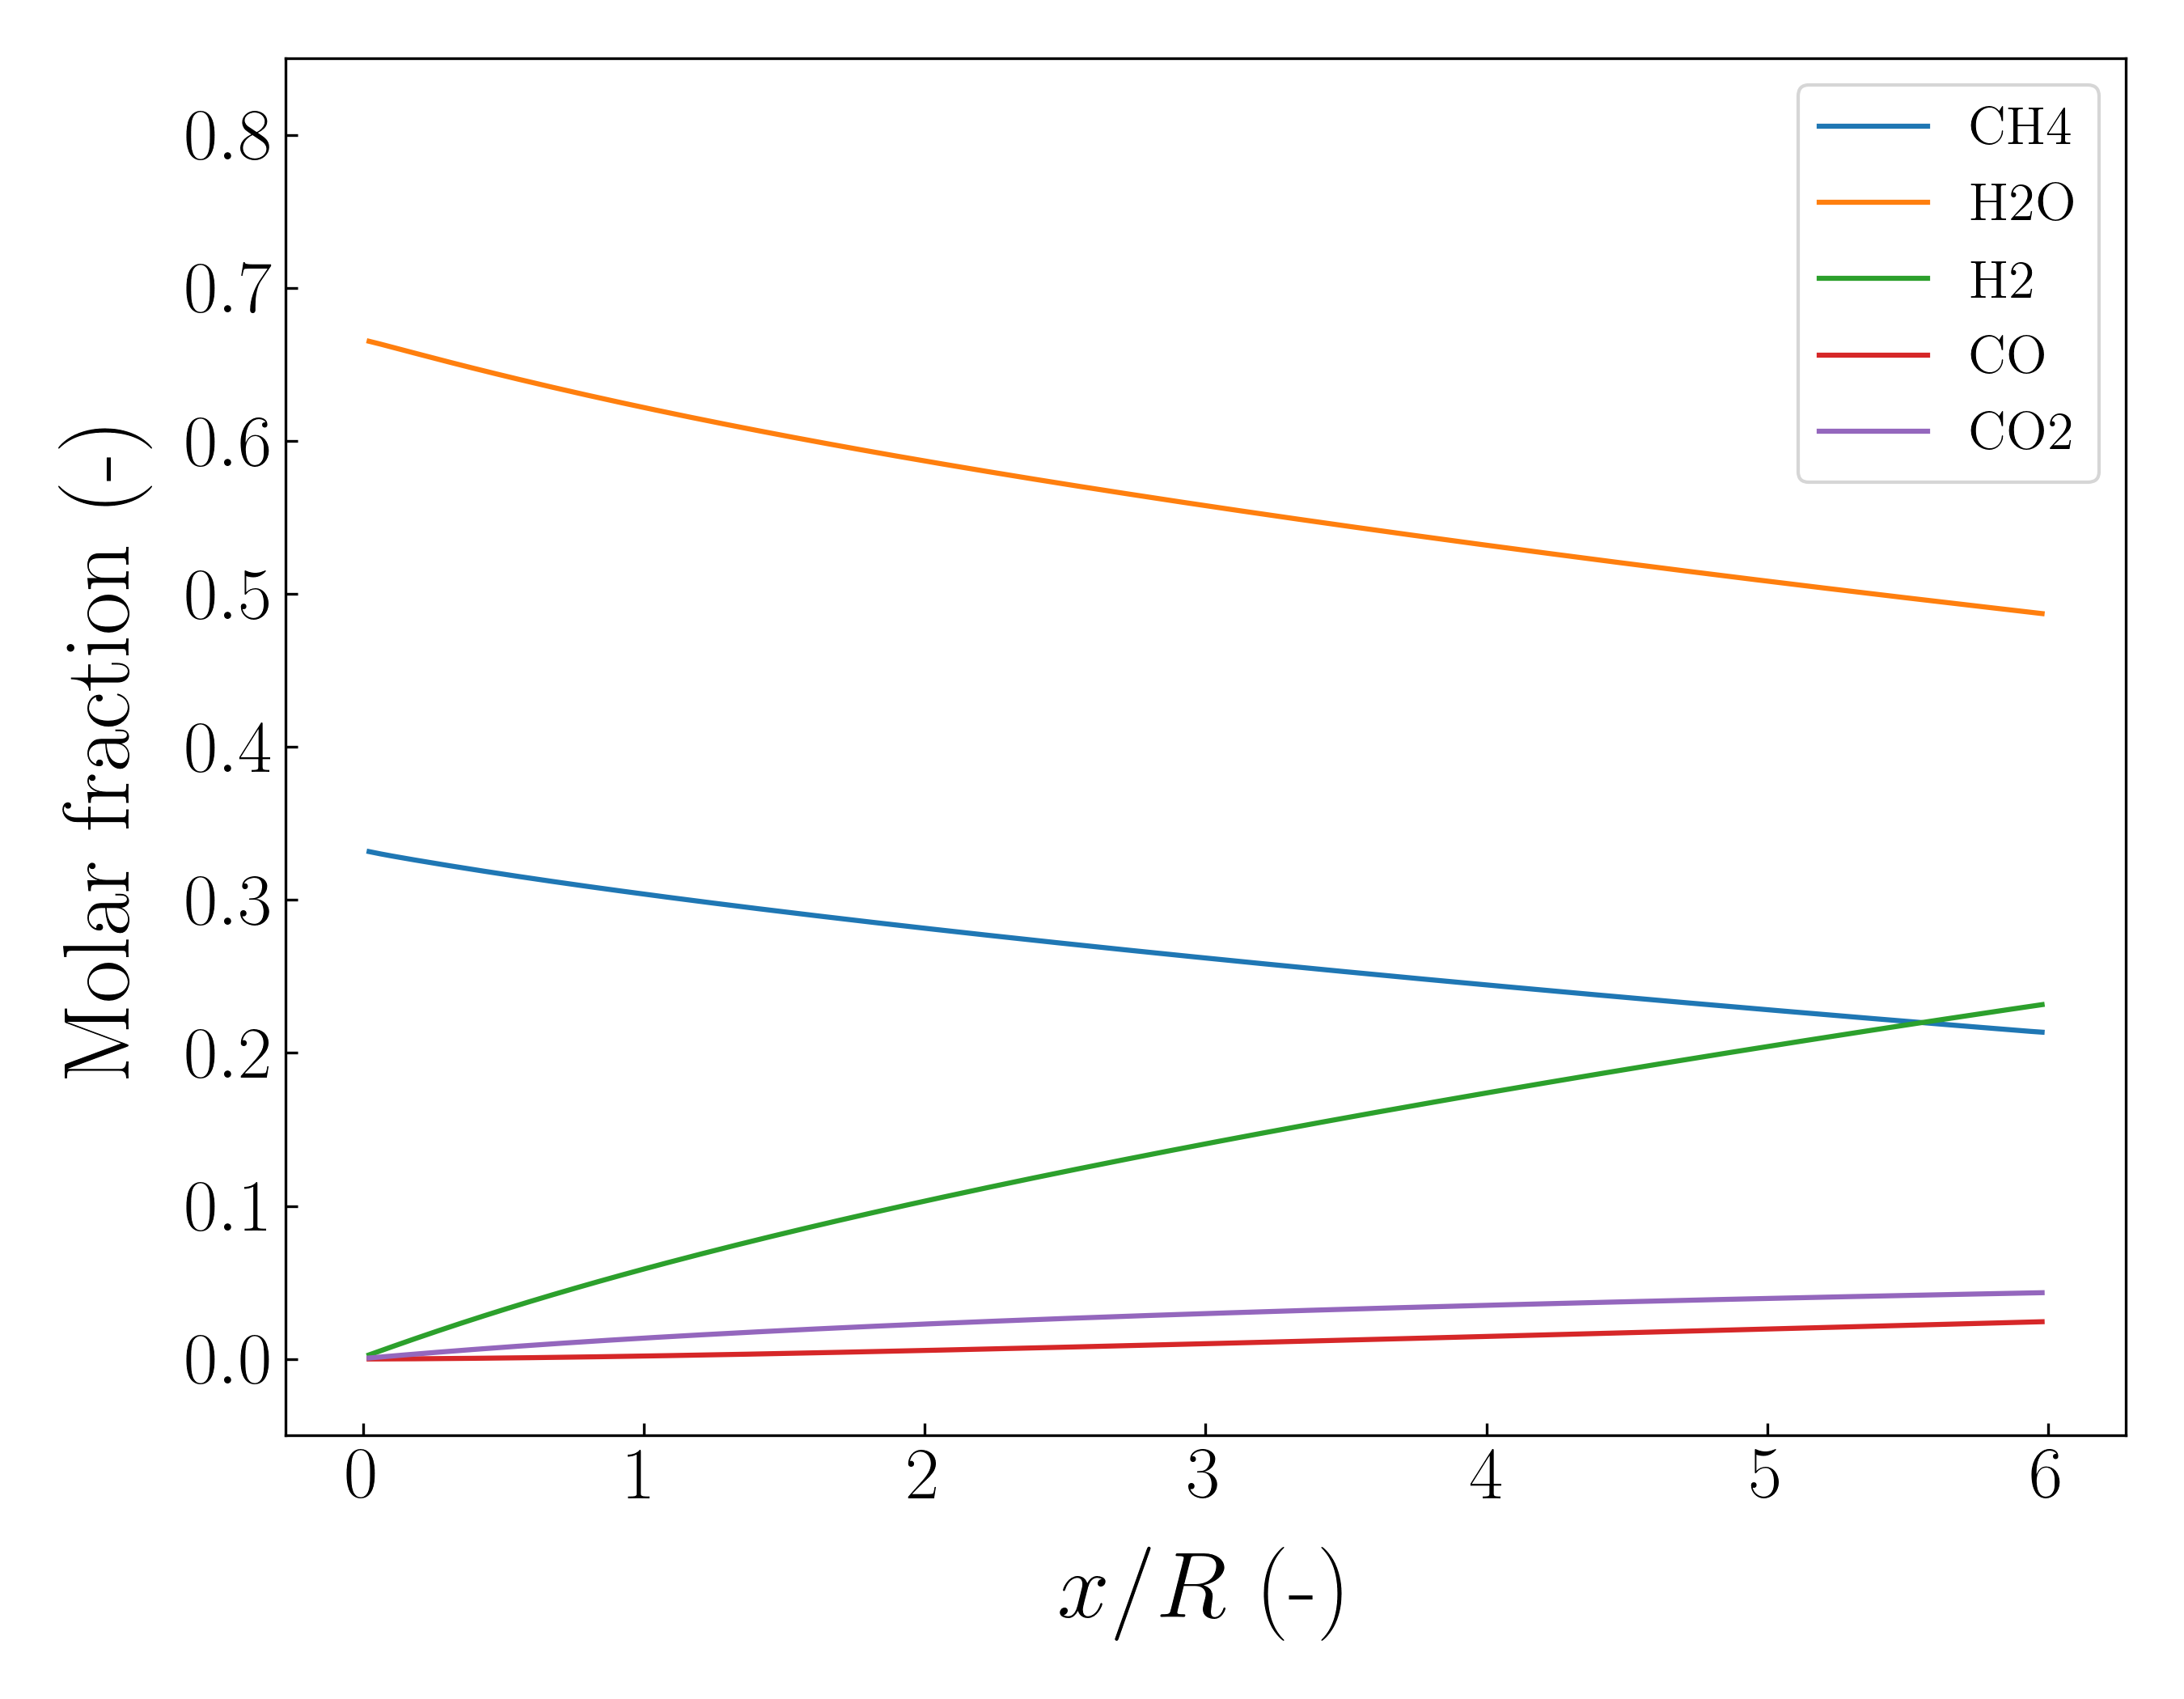
\includegraphics[width=80mm]{results/5/50C_50T/GEN30-AVG.png}
%\caption{\label{fig:5R5050G30-avg} Strategy I - Radius-averaged molar fractions -  30$^{\rm{th}}$ generation ($w_{\rm{CH_4}} = 0.5, w_T = 0.5$, $T_{\rm{in}}$ = 900 K, $u_{\rm{in}}$ = 0.15 m s$^{-1}$, $SC$ = 2.0)}
%\end{figure}
%
%\begin{figure}[h!]
%\centering
%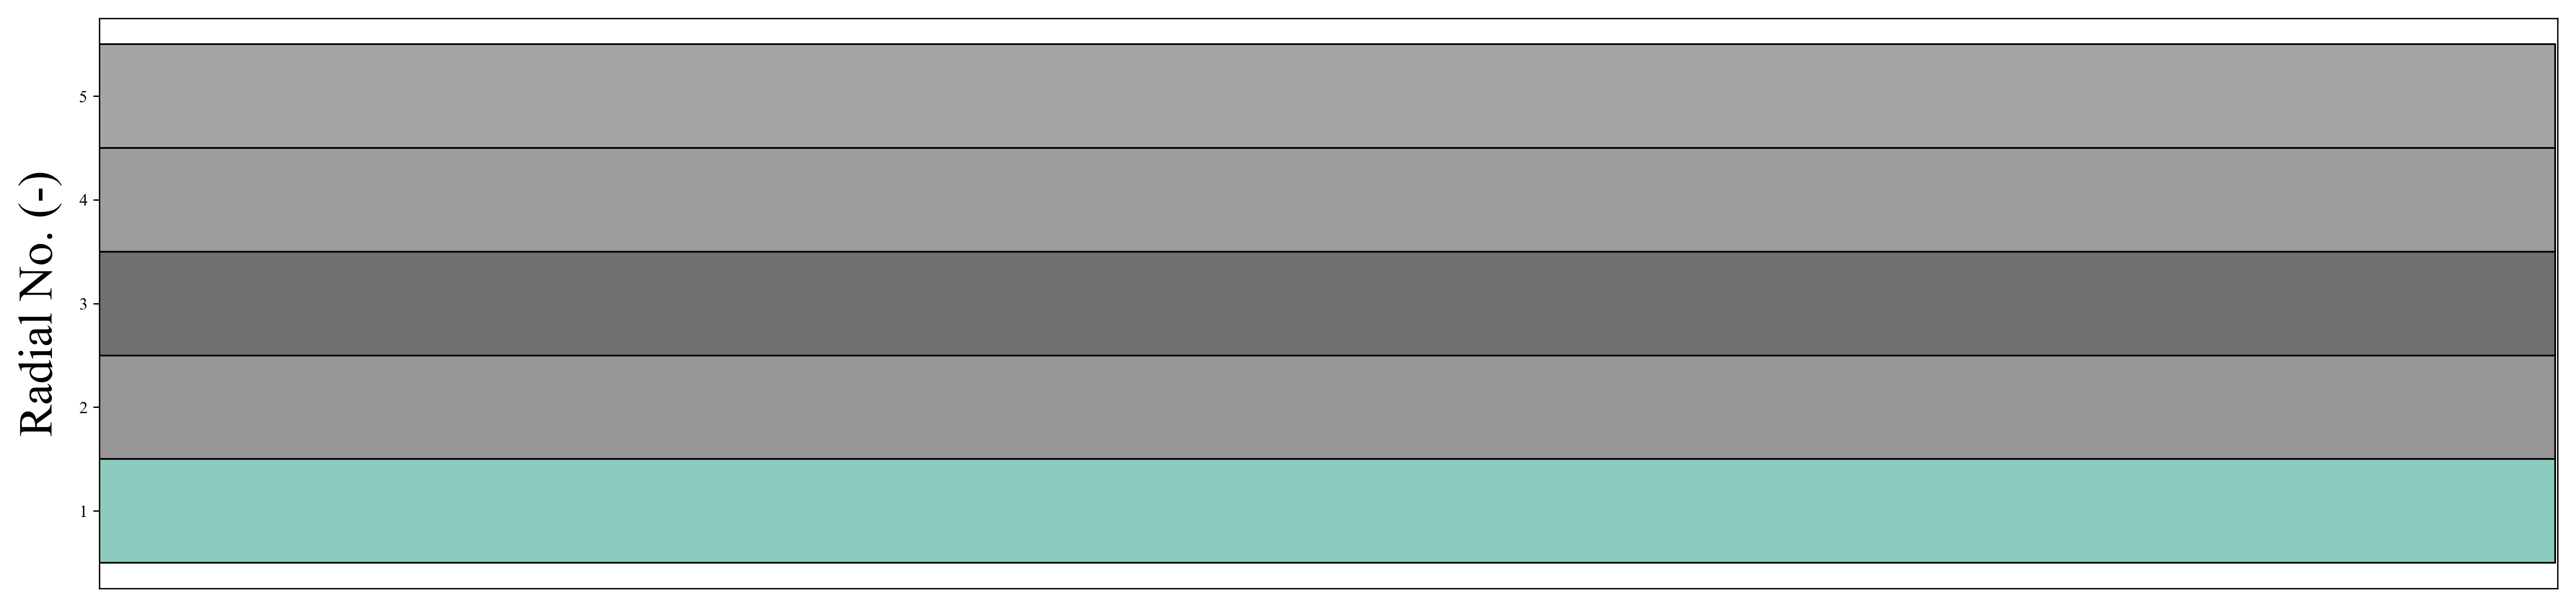
\includegraphics[width=120mm]{results/segments/5seg/50C50T/seg.png}
%\caption{\label{fig:30L6040G1-TField} Strategy I - Segments distribution for 30$^{\rm{th}}$ generation ($w_{\rm{CH_4}} = 0.5, w_T = 0.5$, $T_{\rm{in}}$ = 900 K, $u_{\rm{in}}$ = 0.15 m s$^{-1}$, $SC$ = 2.0)}
%\end{figure}
%
%\begin{figure}[h!]
%\centering
%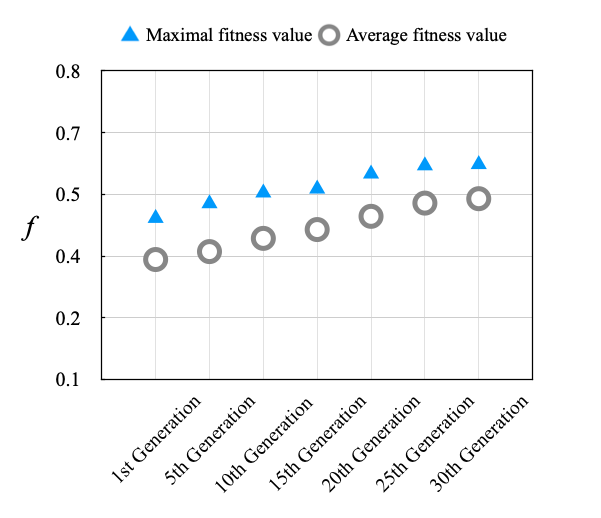
\includegraphics[width=100mm]{results/5/50C_50T.png}
%\caption{\label{fig:5R5050G-fitness} Strategy I - Fitness analysis throughout successive populations ($w_{\rm{CH_4}} = 0.5, w_T = 0.5$, $T_{\rm{in}}$ = 900 K, $u_{\rm{in}}$ = 0.15 m s$^{-1}$, $SC$ = 2.0)}
%\end{figure}
%
%
%\clearpage
%
%
%
%\paragraph{Thermal fitness 40 \%, methane conversion 60 \%} \hspace{0pt} \\
%\noindent 
%
%
%\begin{figure}[h!]
%\centering
%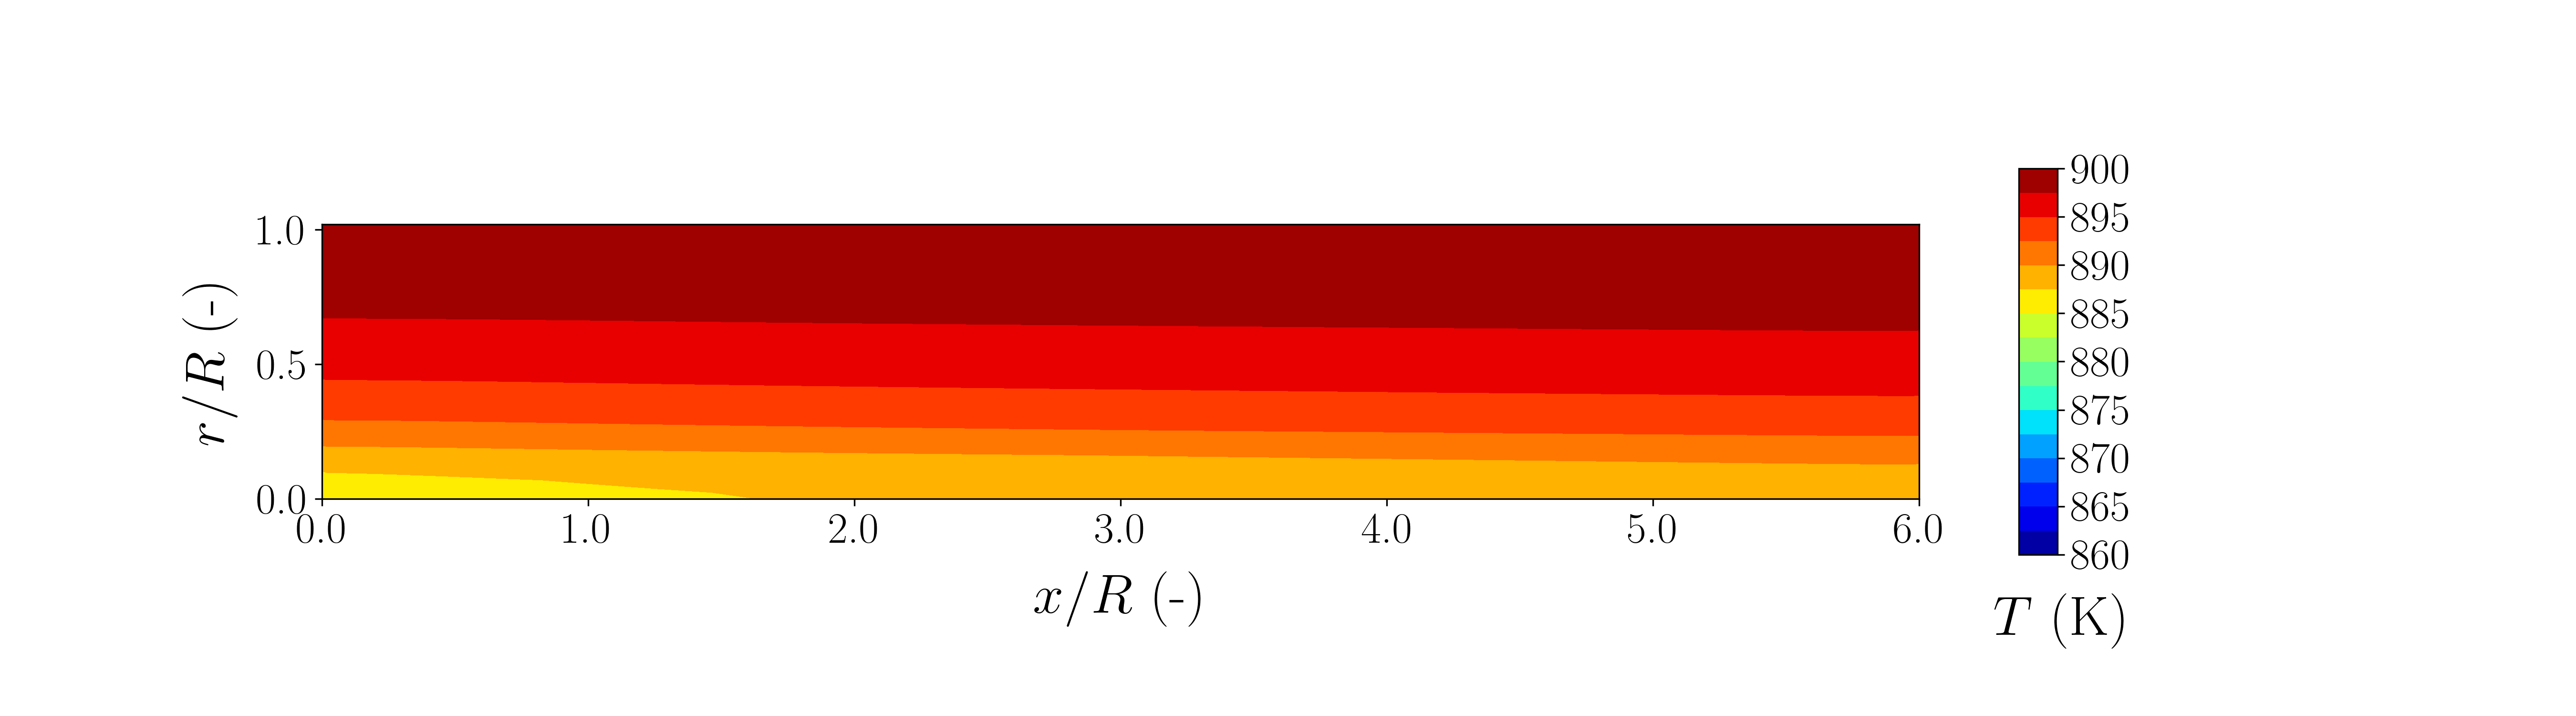
\includegraphics[width=190mm]{results/5/60C_40T/GEN1-TFIELD.png}
%\caption{\label{fig:5R6040G1-TField} Strategy I - Temperature field distribution - 1$^{\rm{st}}$ generation ($w_{\rm{CH_4}} = 0.6, w_T = 0.4$, $T_{\rm{in}}$ = 900 K, $u_{\rm{in}}$ = 0.15 m s$^{-1}$, $SC$ = 2.0)}
%\end{figure}
%
%\begin{figure}[h!]
%\centering
%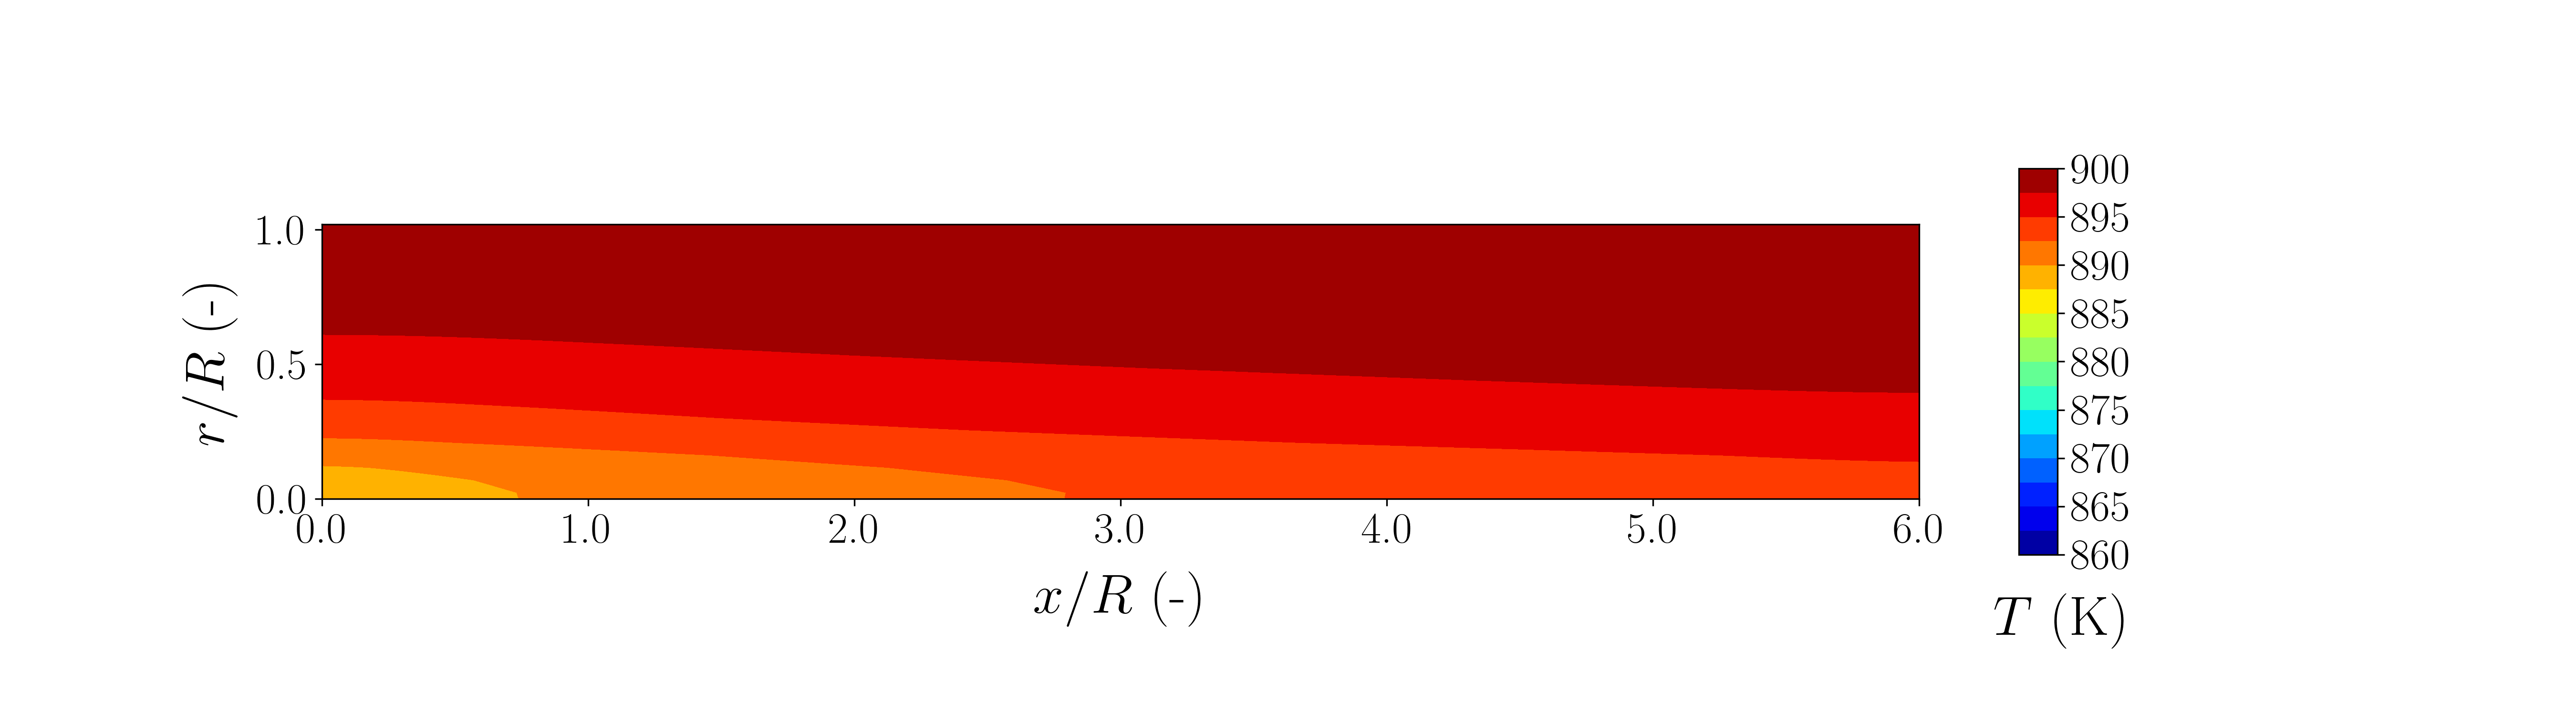
\includegraphics[width=190mm]{results/5/60C_40T/GEN15-TFIELD.png}
%\caption{\label{fig:5R6040G15-TField} Strategy I - Temperature field distribution - 15$^{\rm{th}}$ generation ($w_{\rm{CH_4}} = 0.6, w_T = 0.4$, $T_{\rm{in}}$ = 900 K, $u_{\rm{in}}$ = 0.15 m s$^{-1}$, $SC$ = 2.0)}
%\end{figure}
%
%\begin{figure}[h!]
%\centering
%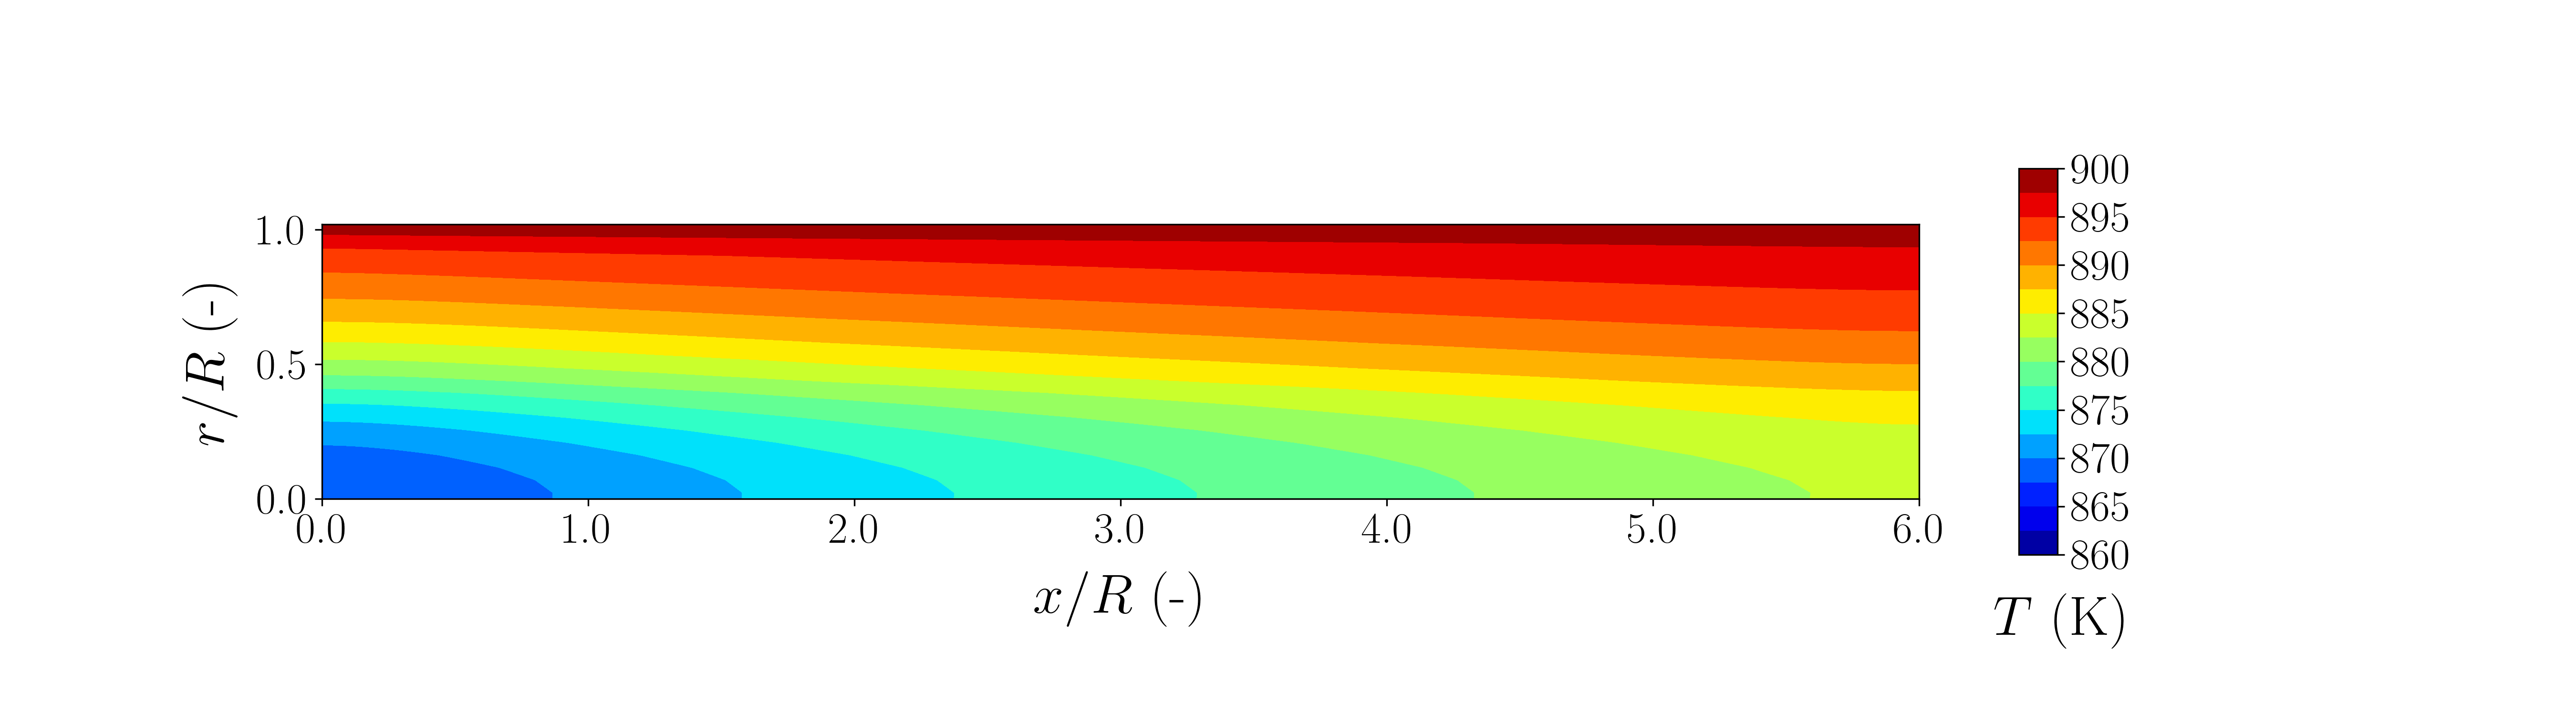
\includegraphics[width=190mm]{results/5/60C_40T/GEN30-TFIELD.png}
%\caption{\label{fig:5R6040G30-TField} Strategy I - Temperature field distribution - 30$^{\rm{th}}$ generation ($w_{\rm{CH_4}} = 0.6, w_T = 0.4$, $T_{\rm{in}}$ = 900 K, $u_{\rm{in}}$ = 0.15 m s$^{-1}$, $SC$ = 2.0)}
%\end{figure}
%
%
%\begin{figure}[h!]
%\centering
%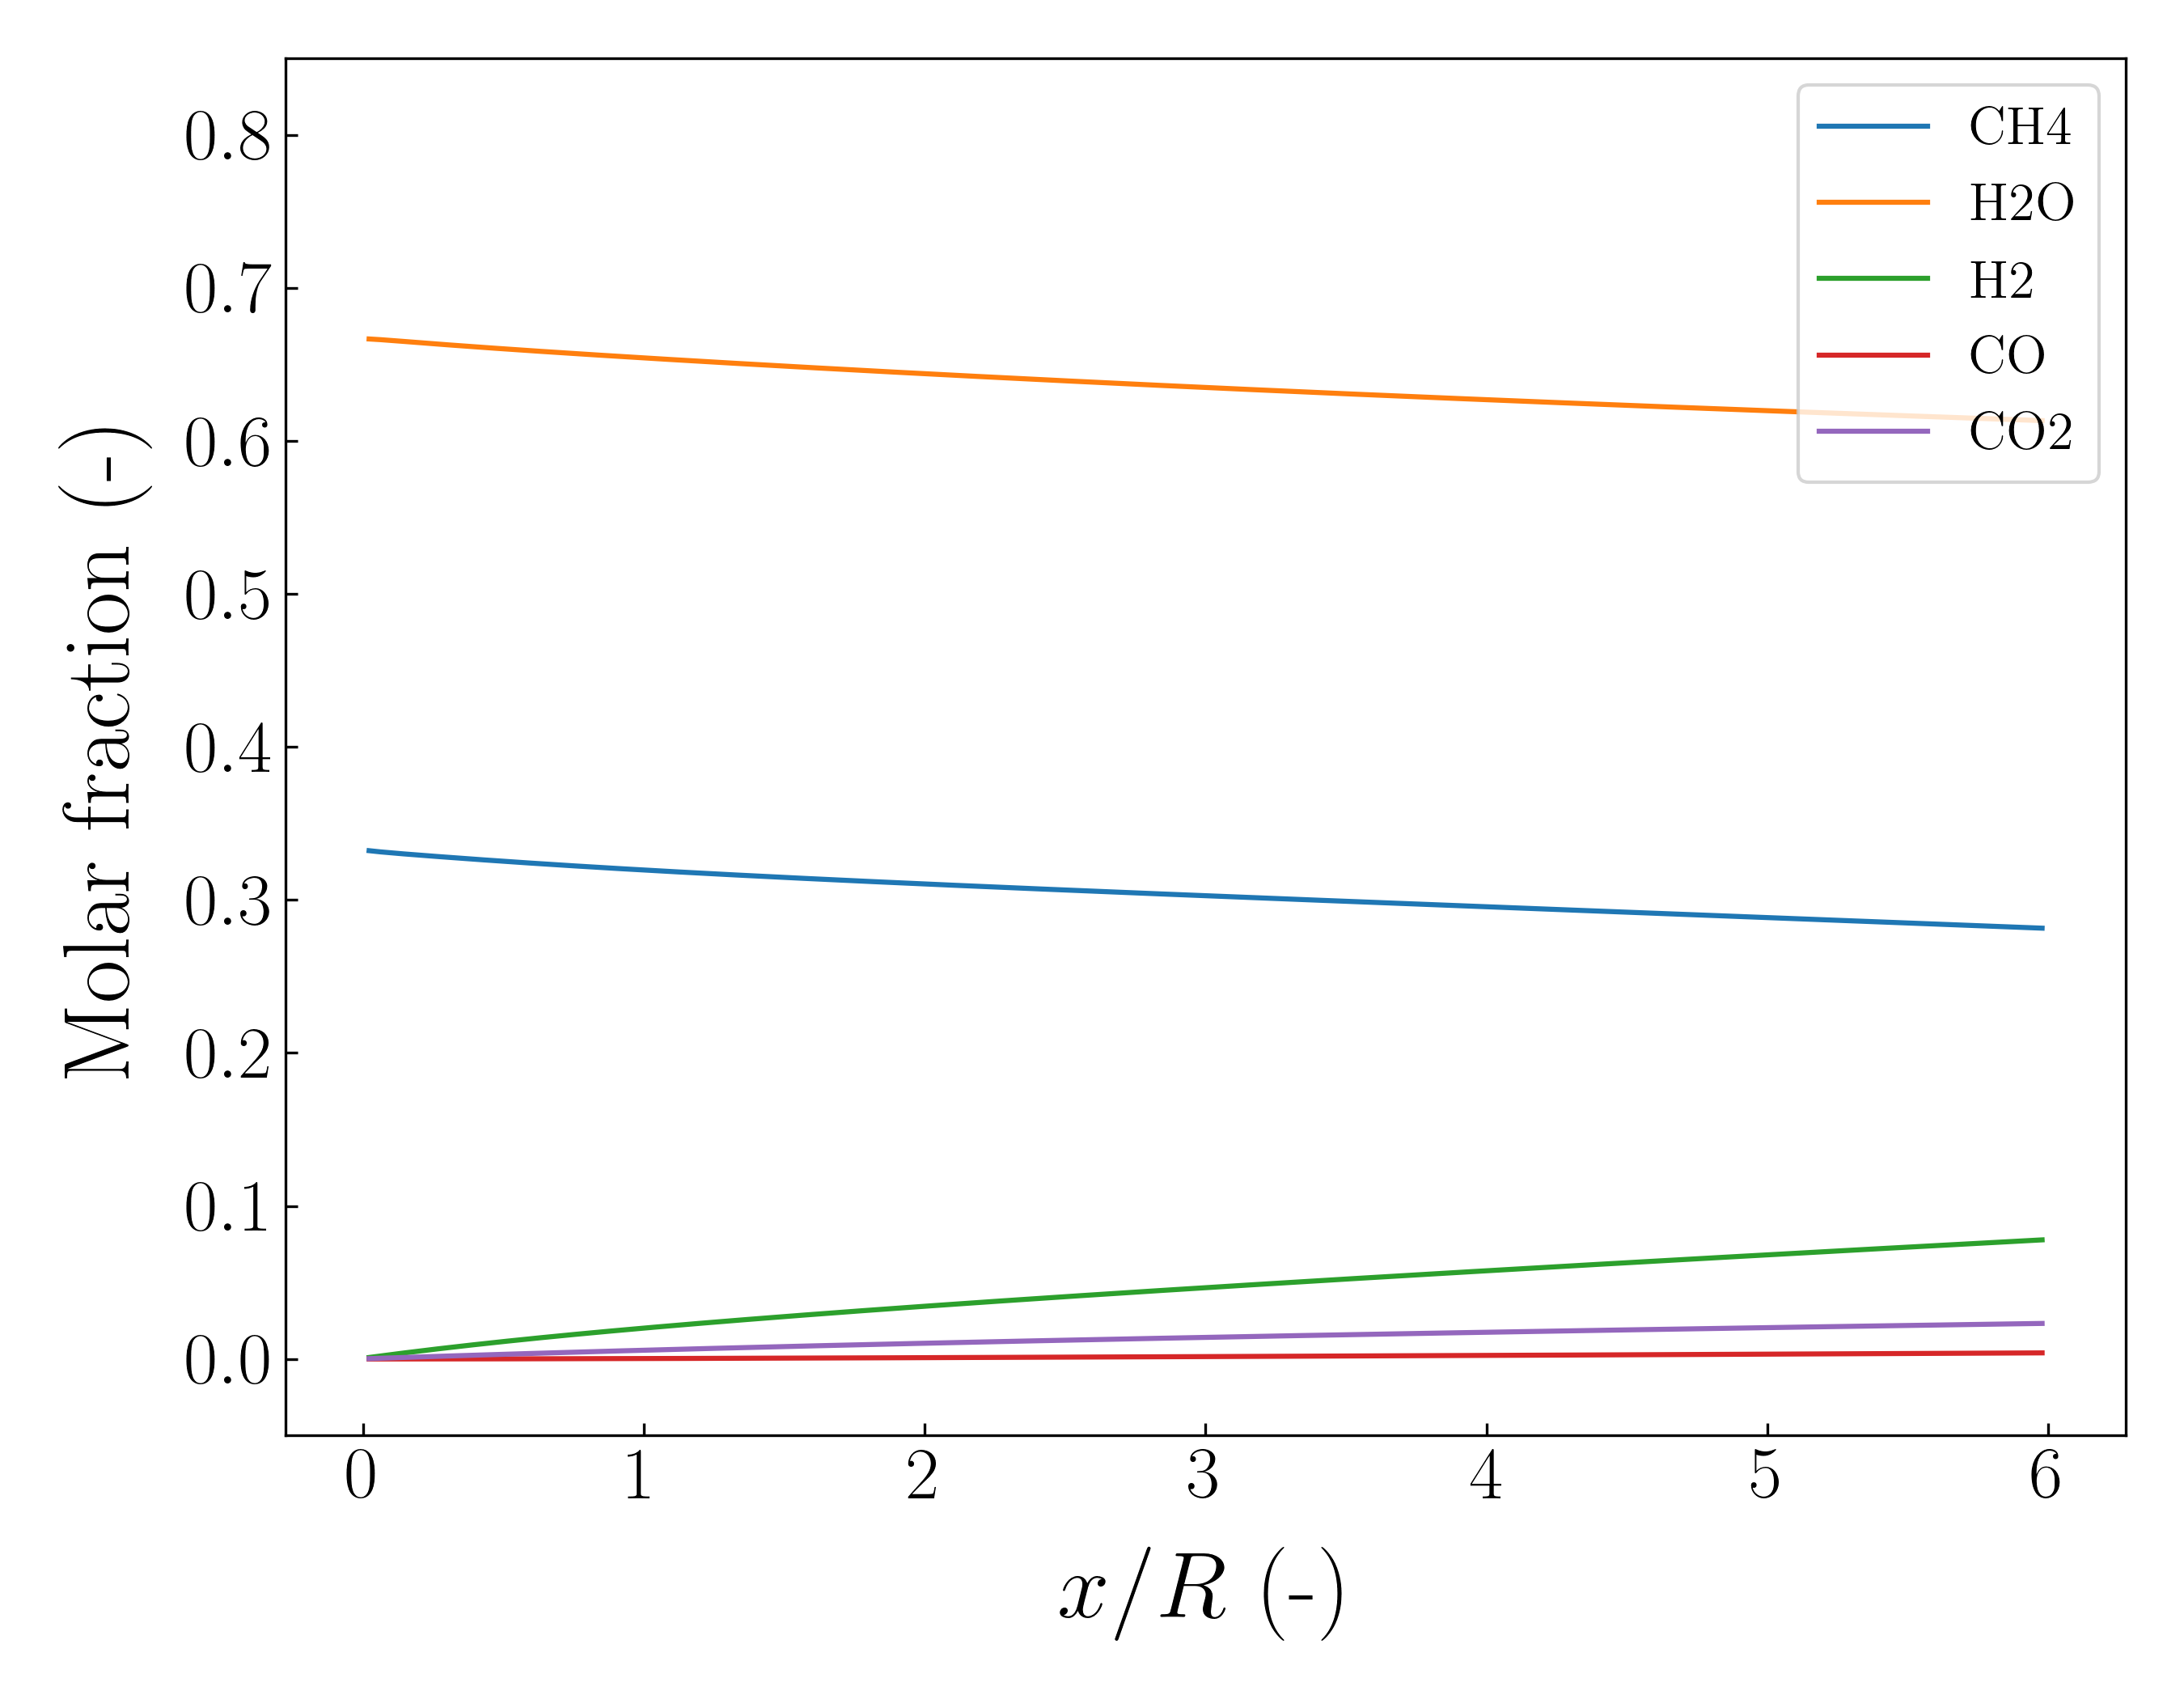
\includegraphics[width=80mm]{results/5/60C_40T/GEN1-AVG.png}
%\caption{\label{fig:5R6040G1-avg} Strategy I - Radius-averaged molar fractions - 1$^{\rm{st}}$ generation ($w_{\rm{CH_4}} = 0.6, w_T = 0.4$, $T_{\rm{in}}$ = 900 K, $u_{\rm{in}}$ = 0.15 m s$^{-1}$, $SC$ = 2.0)}
%\end{figure}
%
%\begin{figure}[h!]
%\centering
%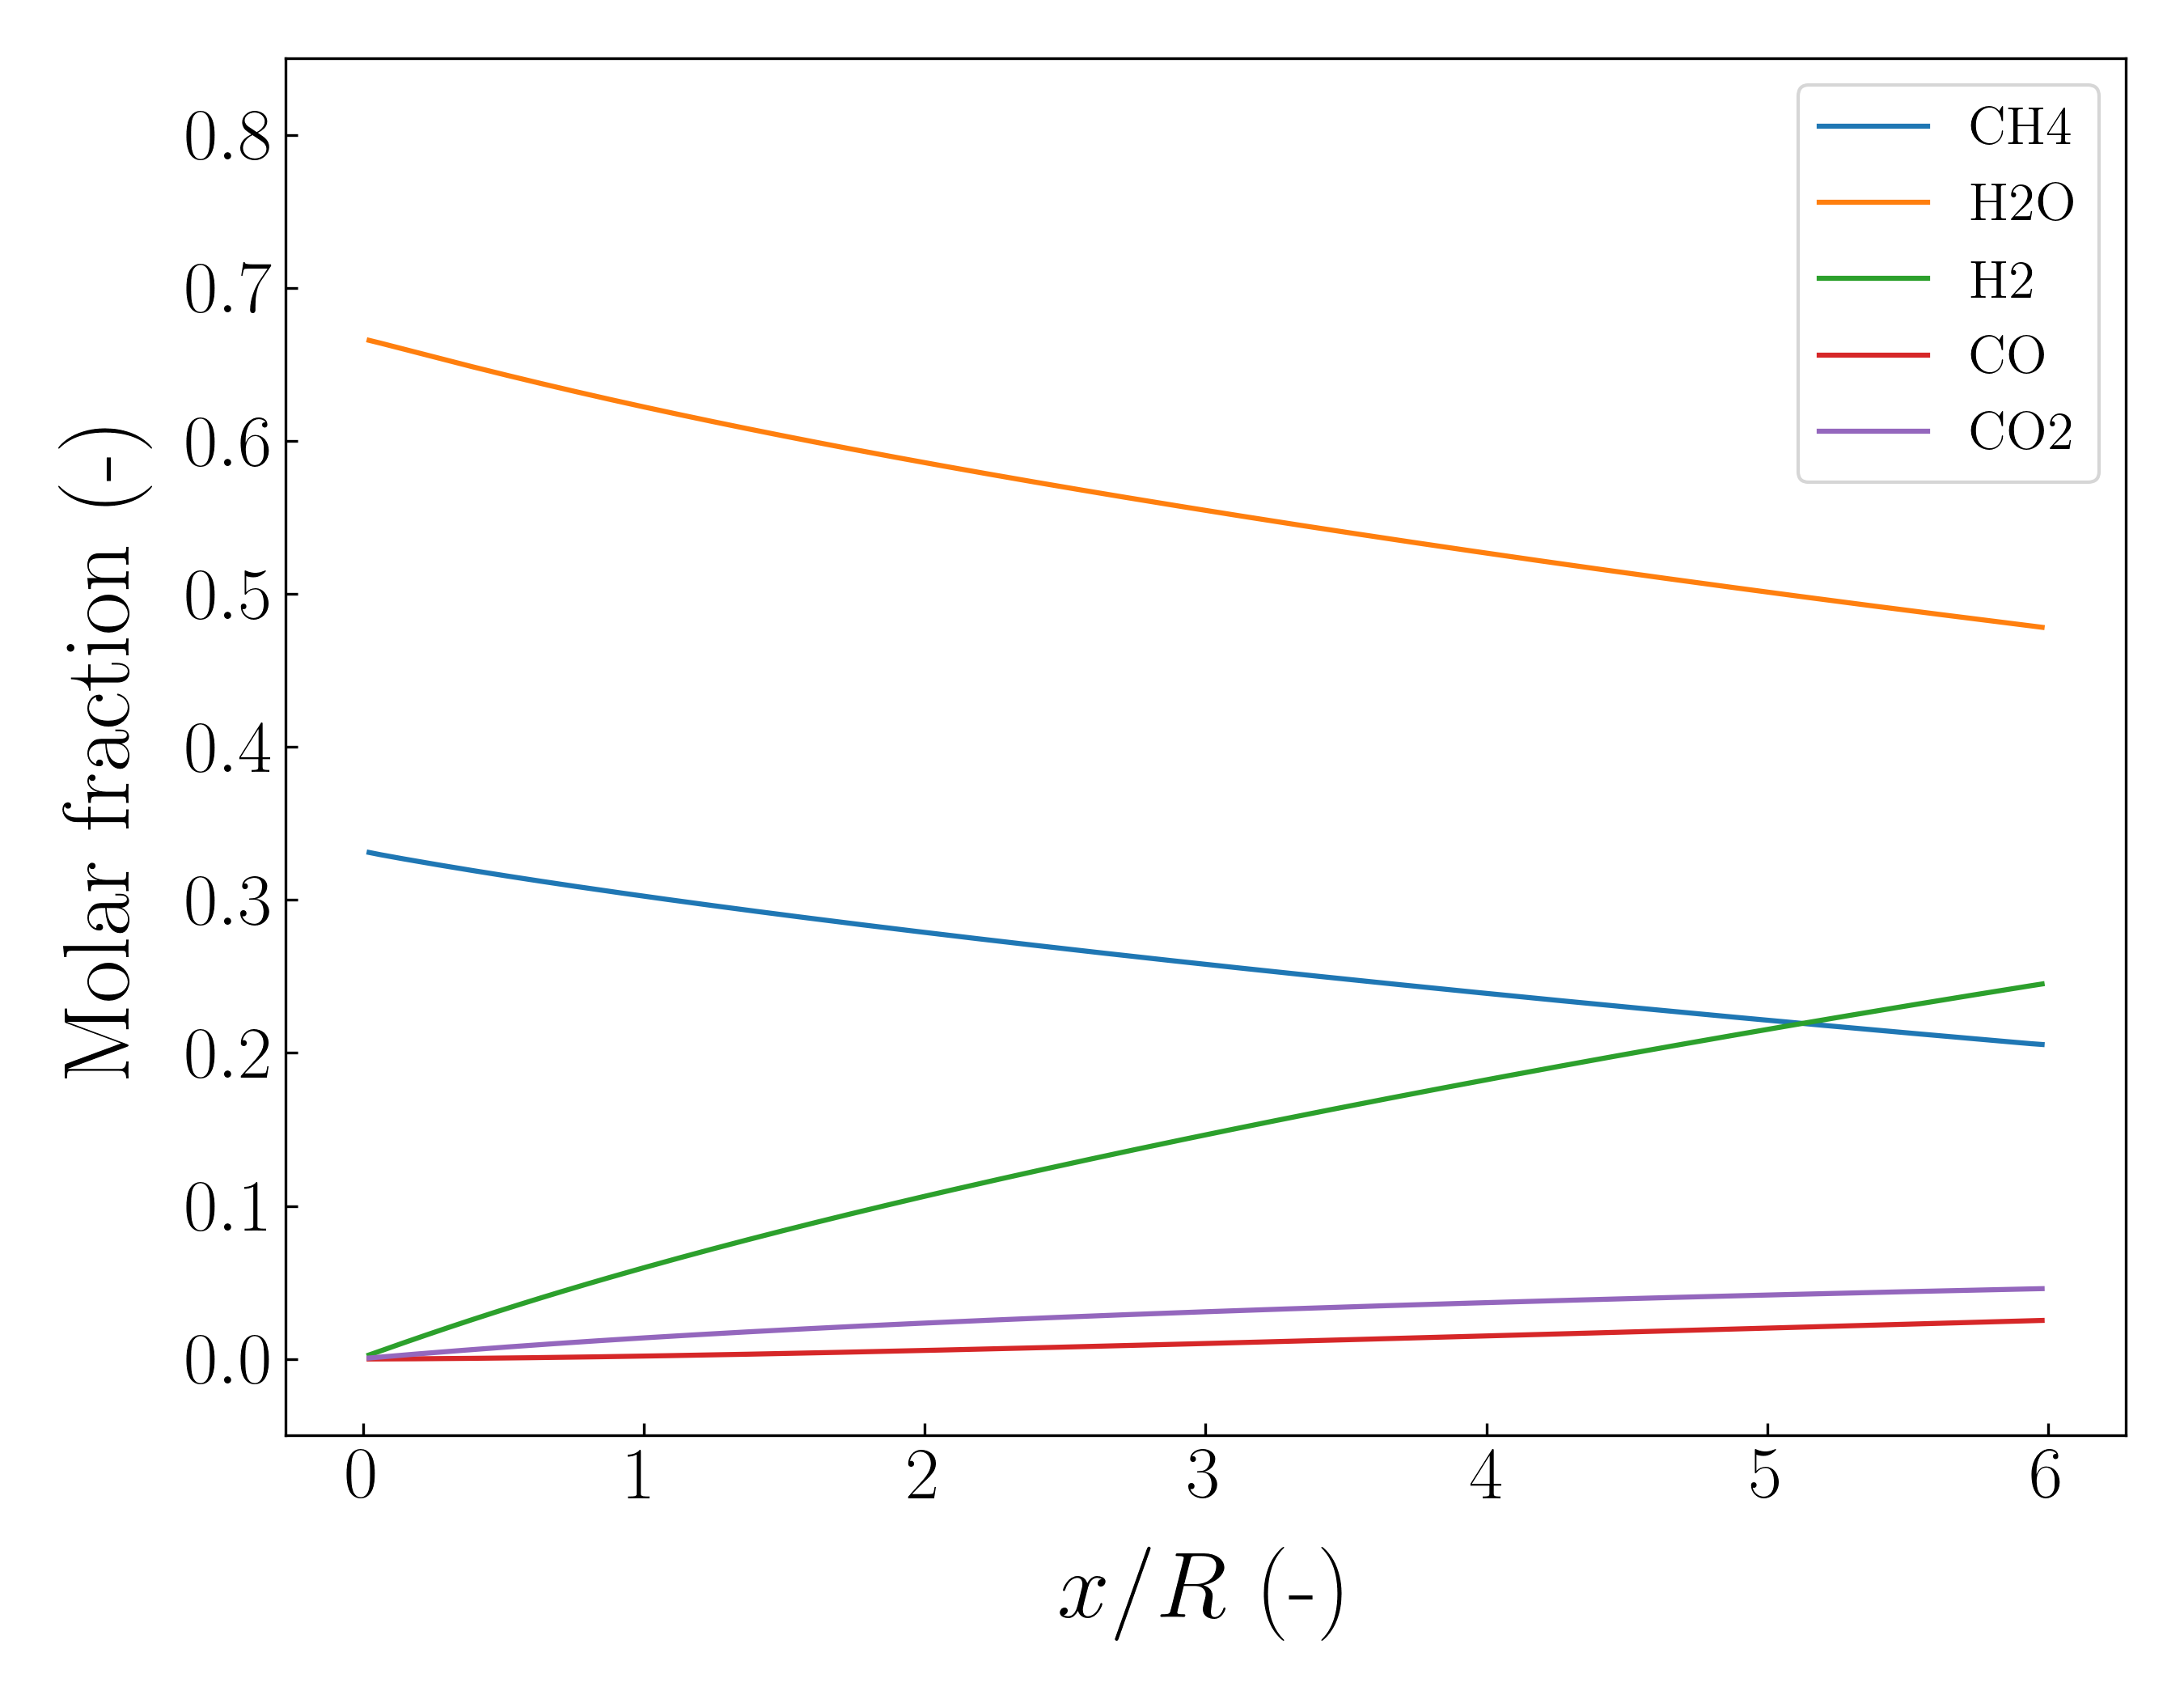
\includegraphics[width=80mm]{results/5/60C_40T/GEN15-AVG.png}
%\caption{\label{fig:5R6040G15-avg} Strategy I - Radius-averaged molar fractions - 15$^{\rm{th}}$ generation ($w_{\rm{CH_4}} = 0.6, w_T = 0.4$, $T_{\rm{in}}$ = 900 K, $u_{\rm{in}}$ = 0.15 m s$^{-1}$, $SC$ = 2.0)}
%\end{figure}
%
%\begin{figure}[h!]
%\centering
%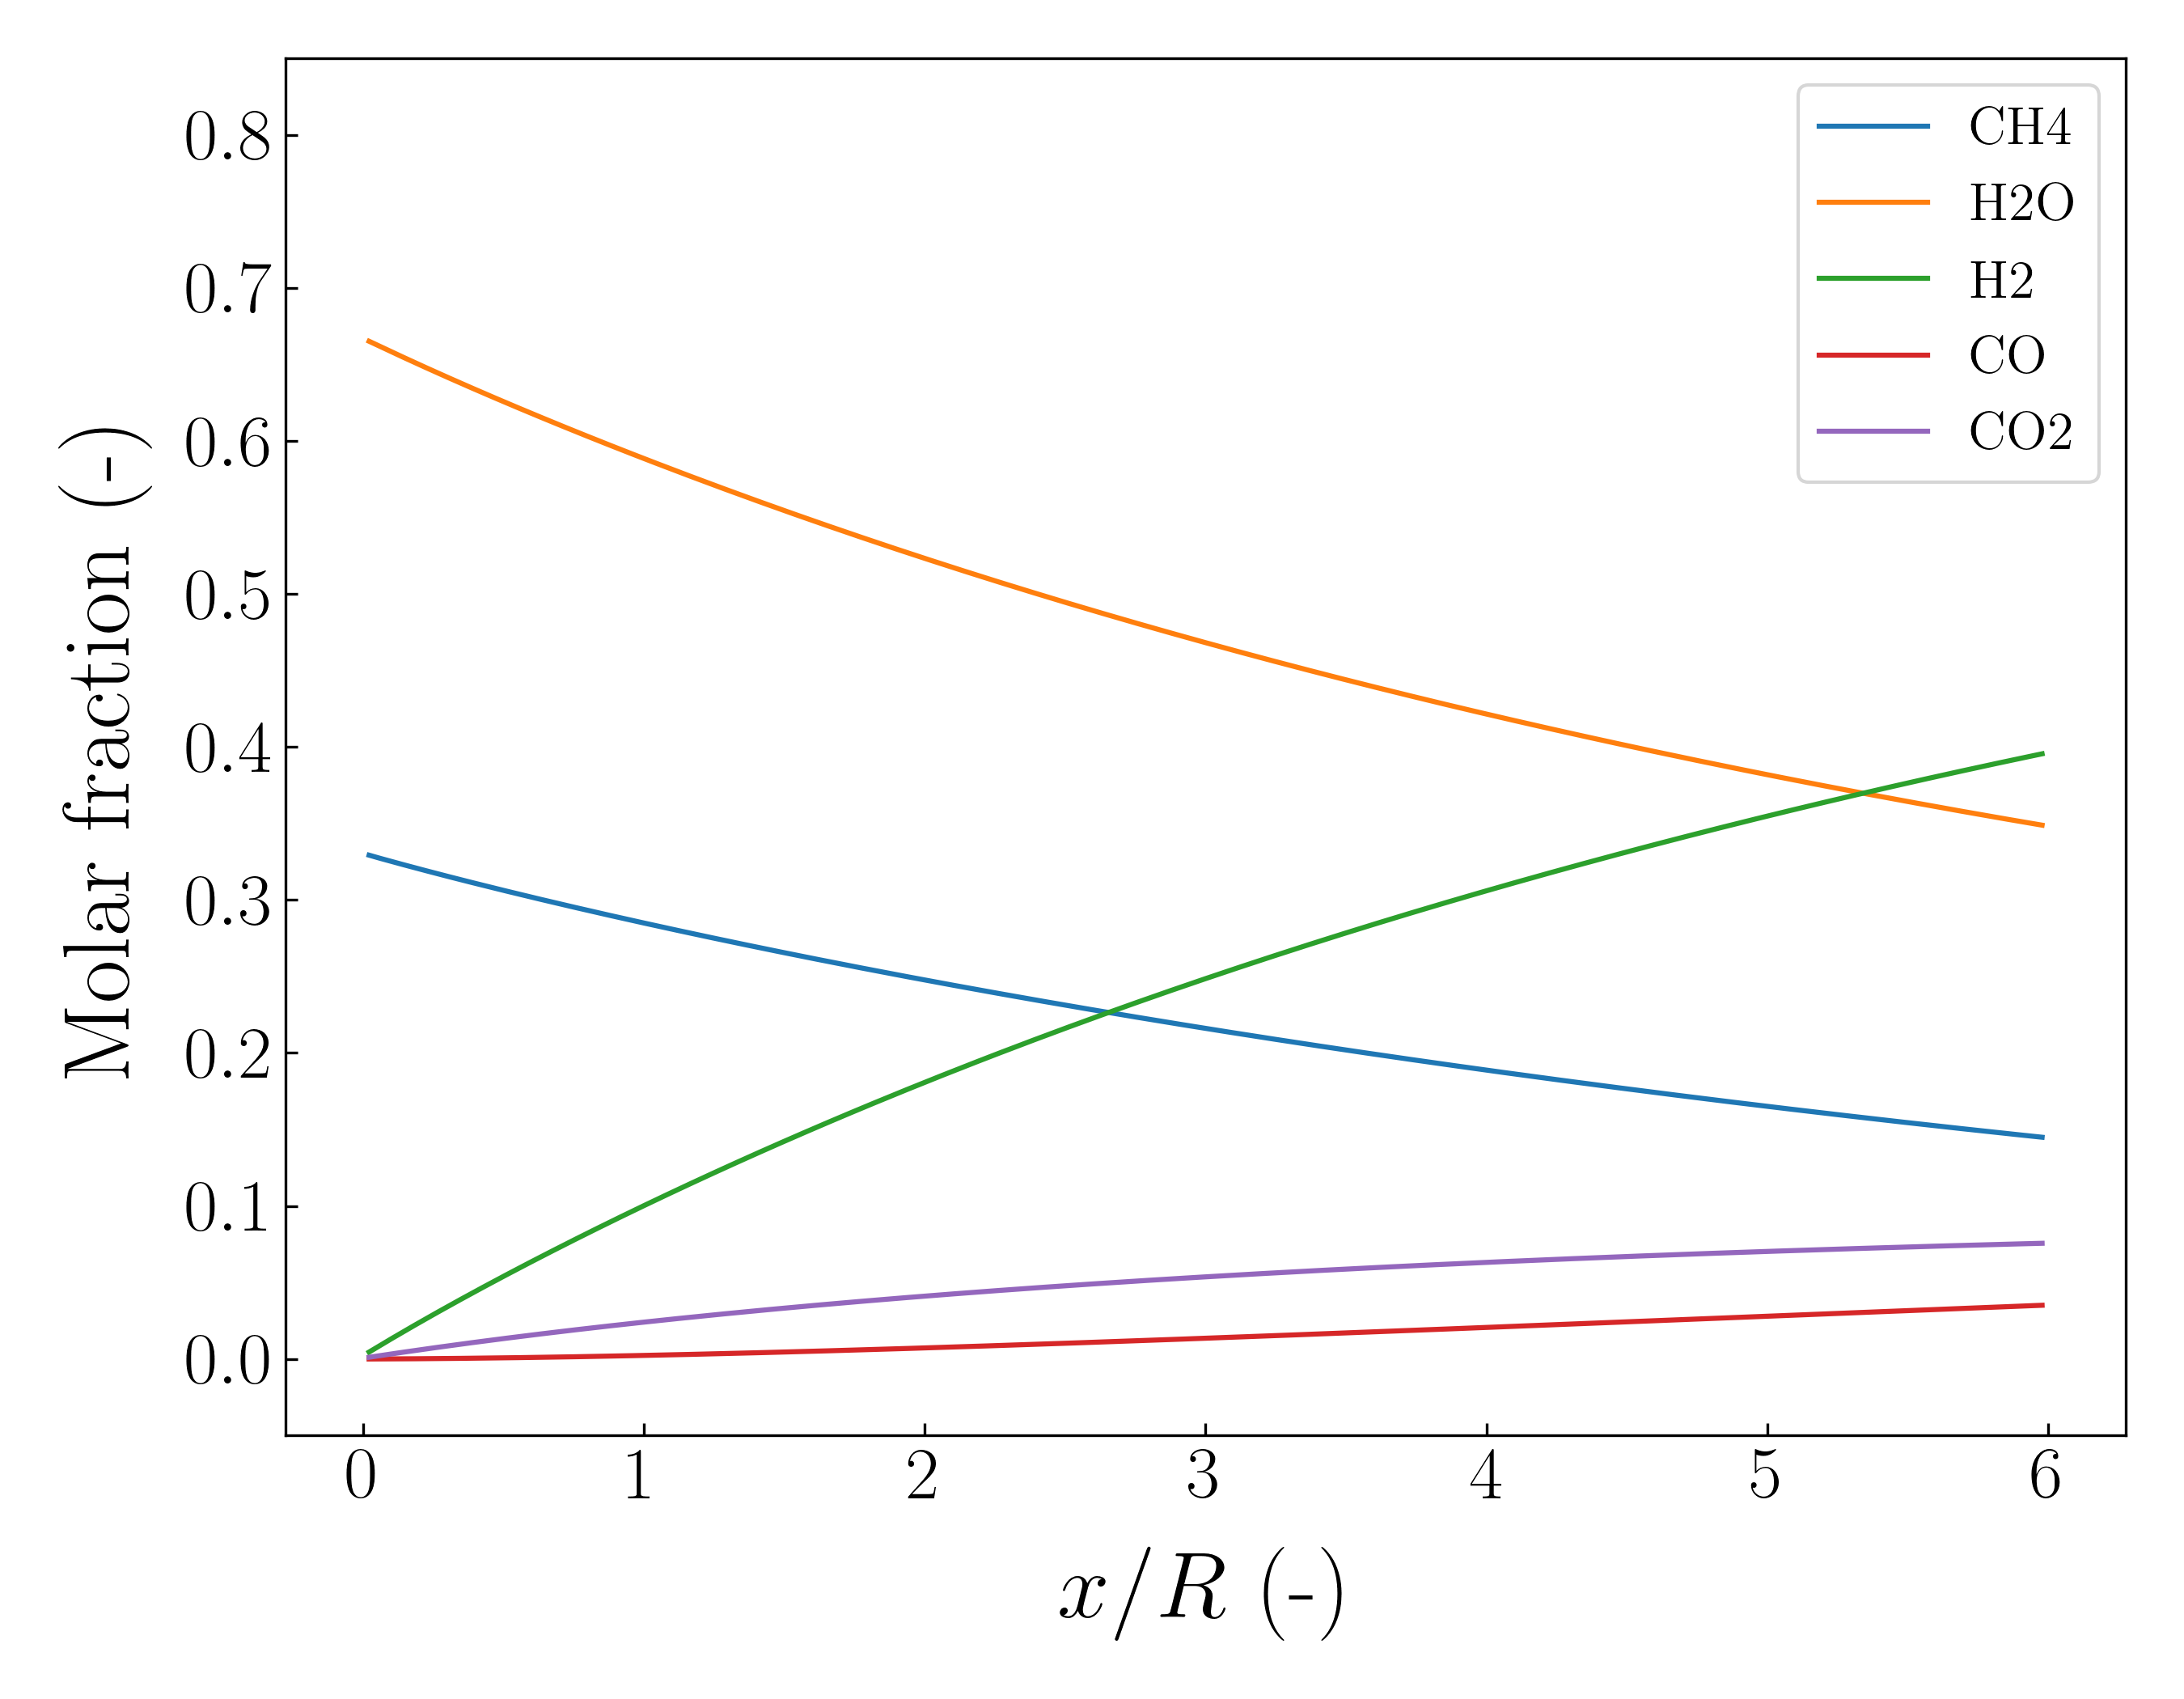
\includegraphics[width=80mm]{results/5/60C_40T/GEN30-AVG.png}
%\caption{\label{fig:5R6040G30-avg} Strategy I - Radius-averaged molar fractions -  30$^{\rm{th}}$ generation ($w_{\rm{CH_4}} = 0.6, w_T = 0.4$, $T_{\rm{in}}$ = 900 K, $u_{\rm{in}}$ = 0.15 m s$^{-1}$, $SC$ = 2.0)}
%\end{figure}
%
%\begin{figure}[h!]
%\centering
%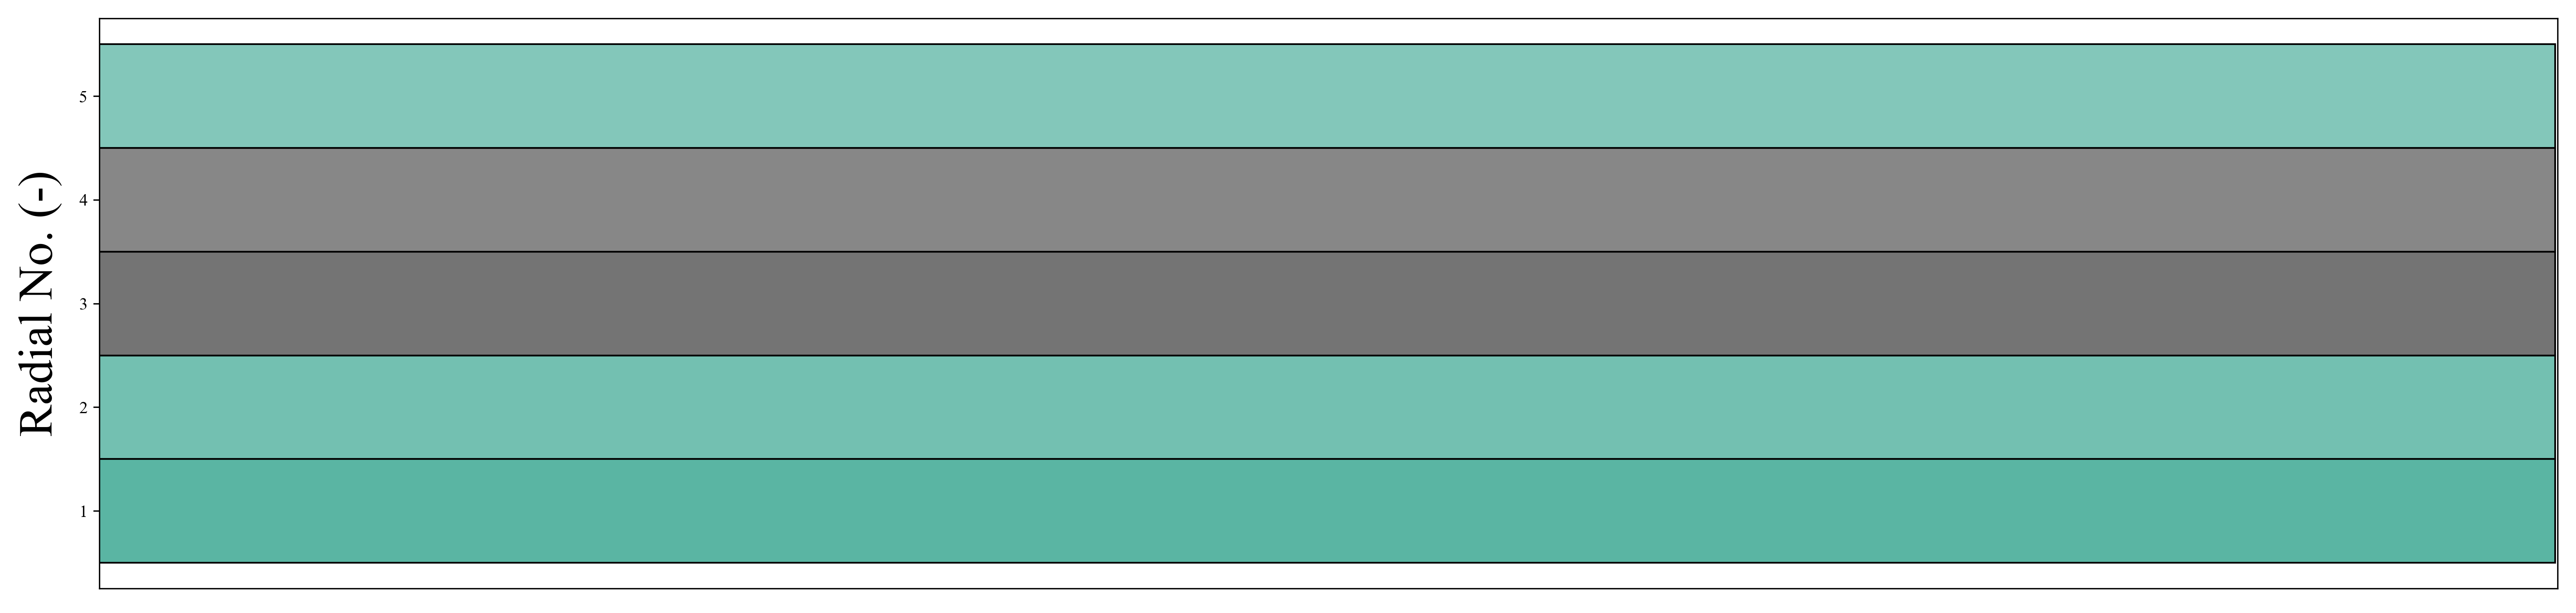
\includegraphics[width=120mm]{results/segments/5seg/60C40T/seg.png}
%\caption{\label{fig:30L6040G1-TField} Strategy I - Segments distribution for 30$^{\rm{th}}$ generation ($w_{\rm{CH_4}} = 0.6, w_T = 0.4$, $T_{\rm{in}}$ = 900 K, $u_{\rm{in}}$ = 0.15 m s$^{-1}$, $SC$ = 2.0)}
%\end{figure}
%
%\begin{figure}[h!]
%\centering
%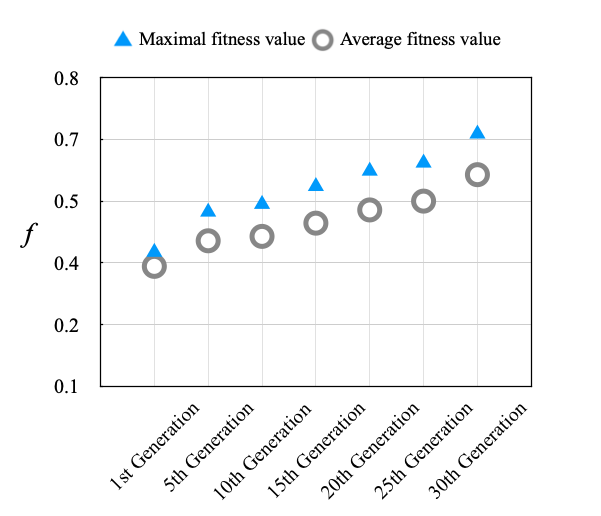
\includegraphics[width=100mm]{results/5/60C_40T.png}
%\caption{\label{fig:5R6040G-fitness} Strategy I - Fitness analysis throughout successive populations ($w_{\rm{CH_4}} = 0.6, w_T = 0.4$, $T_{\rm{in}}$ = 900 K, $u_{\rm{in}}$ = 0.15 m s$^{-1}$, $SC$ = 2.0)}
%\end{figure}
%
%\clearpage
%
%
%\paragraph{Thermal fitness 20 \%, methane conversion 80 \%} \hspace{0pt} \\
%\noindent 
%
%
%
%\begin{figure}[h!]
%\centering
%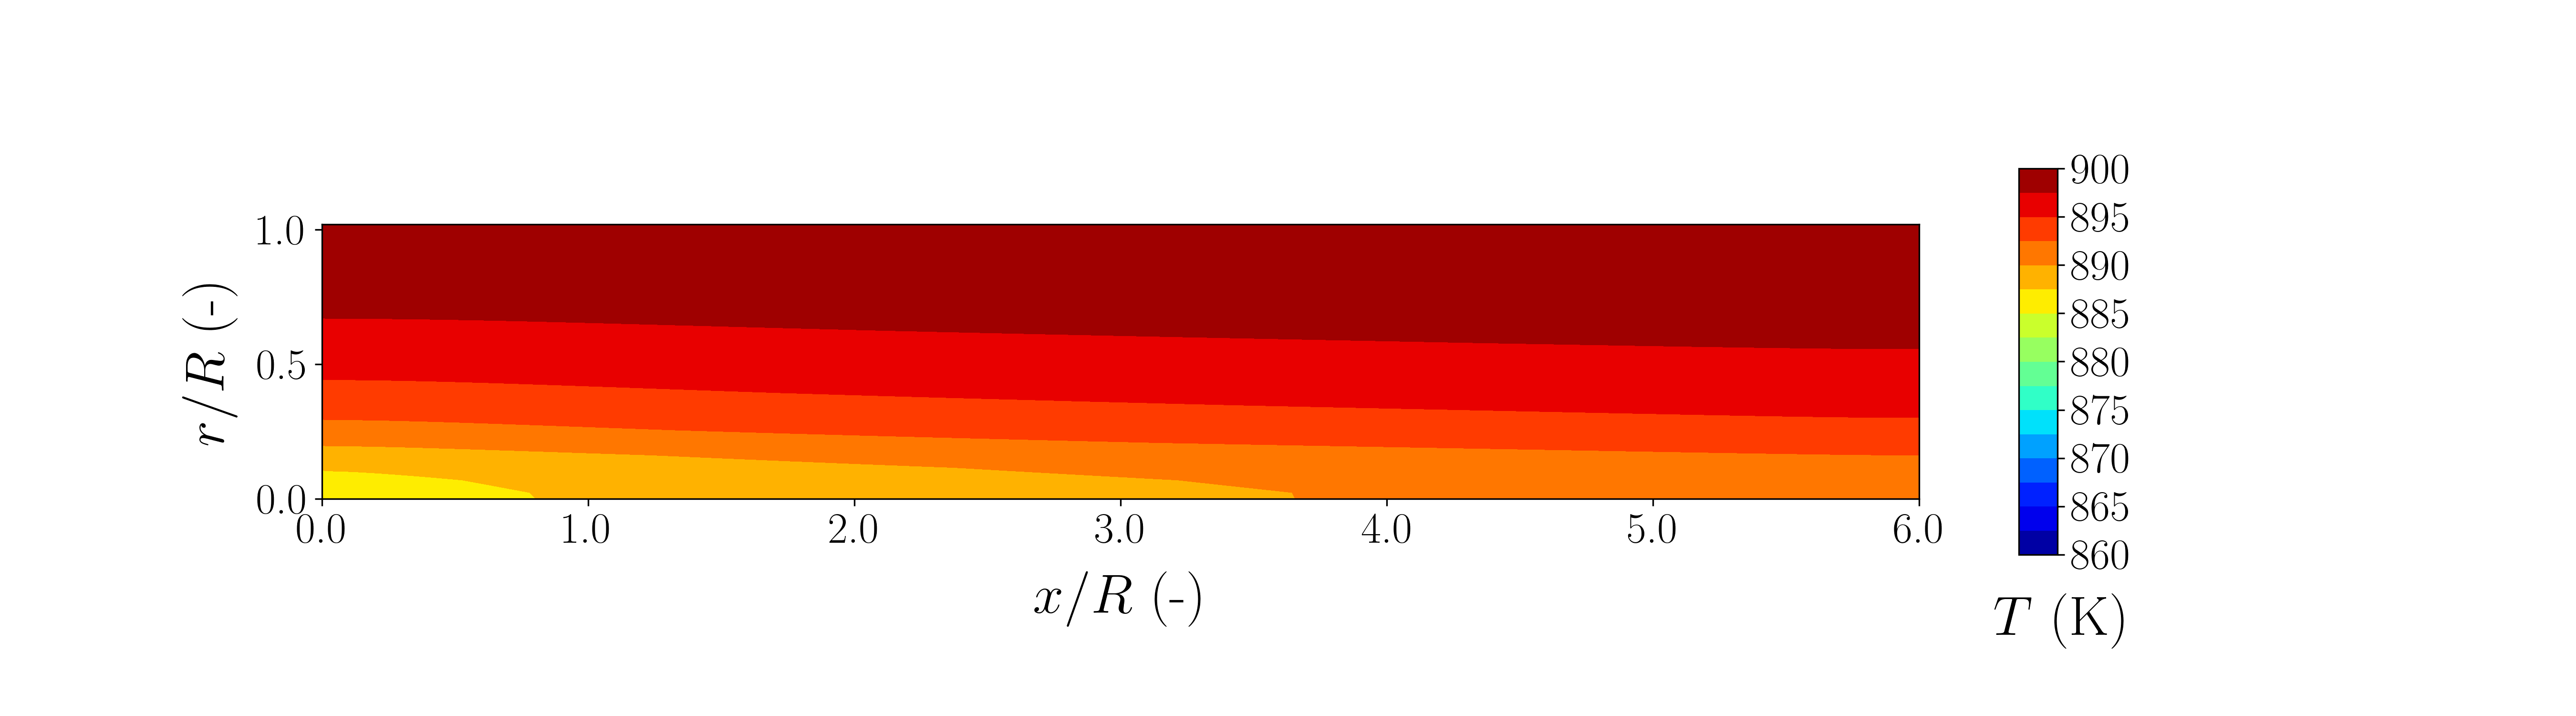
\includegraphics[width=190mm]{results/5/80C_20T/GEN1-TFIELD.png}
%\caption{\label{fig:5R8020G1-TField} Strategy I - Temperature field distribution - 1$^{\rm{st}}$ generation ($w_{\rm{CH_4}} = 0.8, w_T = 0.2$, $T_{\rm{in}}$ = 900 K, $u_{\rm{in}}$ = 0.15 m s$^{-1}$, $SC$ = 2.0)}
%\end{figure}
%
%\begin{figure}[h!]
%\centering
%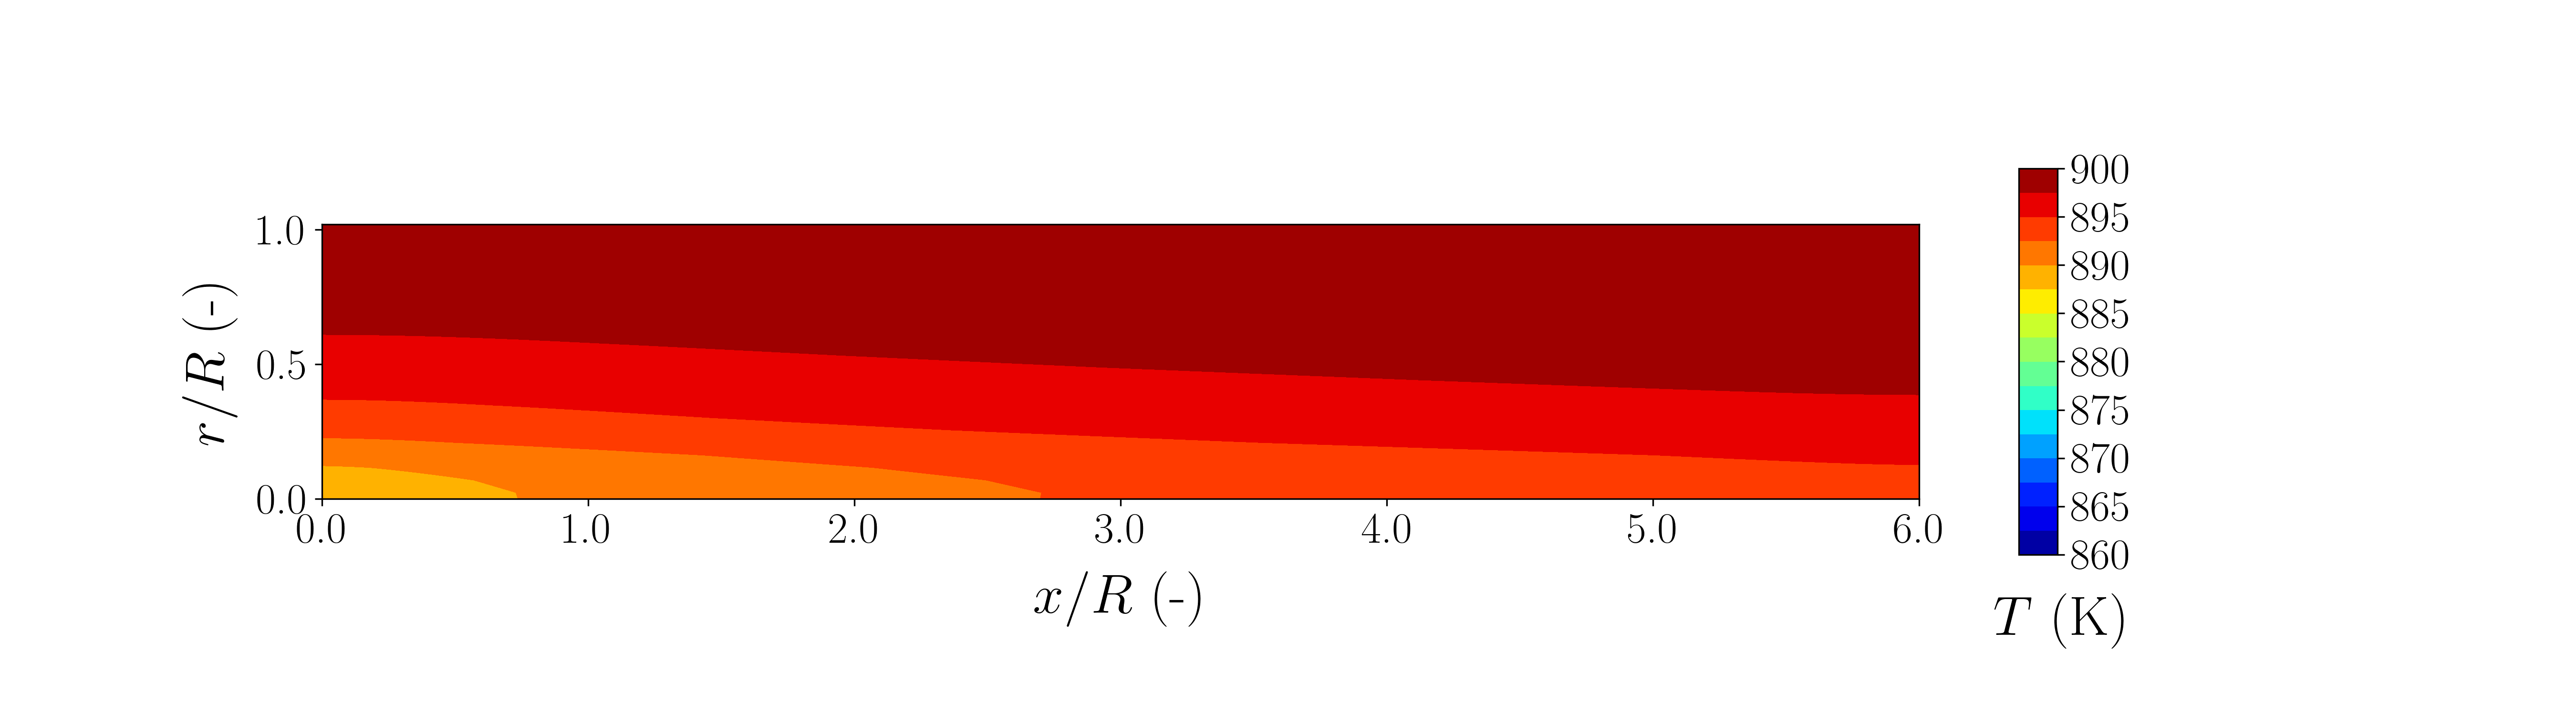
\includegraphics[width=190mm]{results/5/80C_20T/GEN15-TFIELD.png}
%\caption{\label{fig:5R8020G15-TField} Strategy I - Temperature field distribution - 15$^{\rm{th}}$ generation ($w_{\rm{CH_4}} = 0.8, w_T = 0.2$, $T_{\rm{in}}$ = 900 K, $u_{\rm{in}}$ = 0.15 m s$^{-1}$, $SC$ = 2.0)}
%\end{figure}
%
%\begin{figure}[h!]
%\centering
%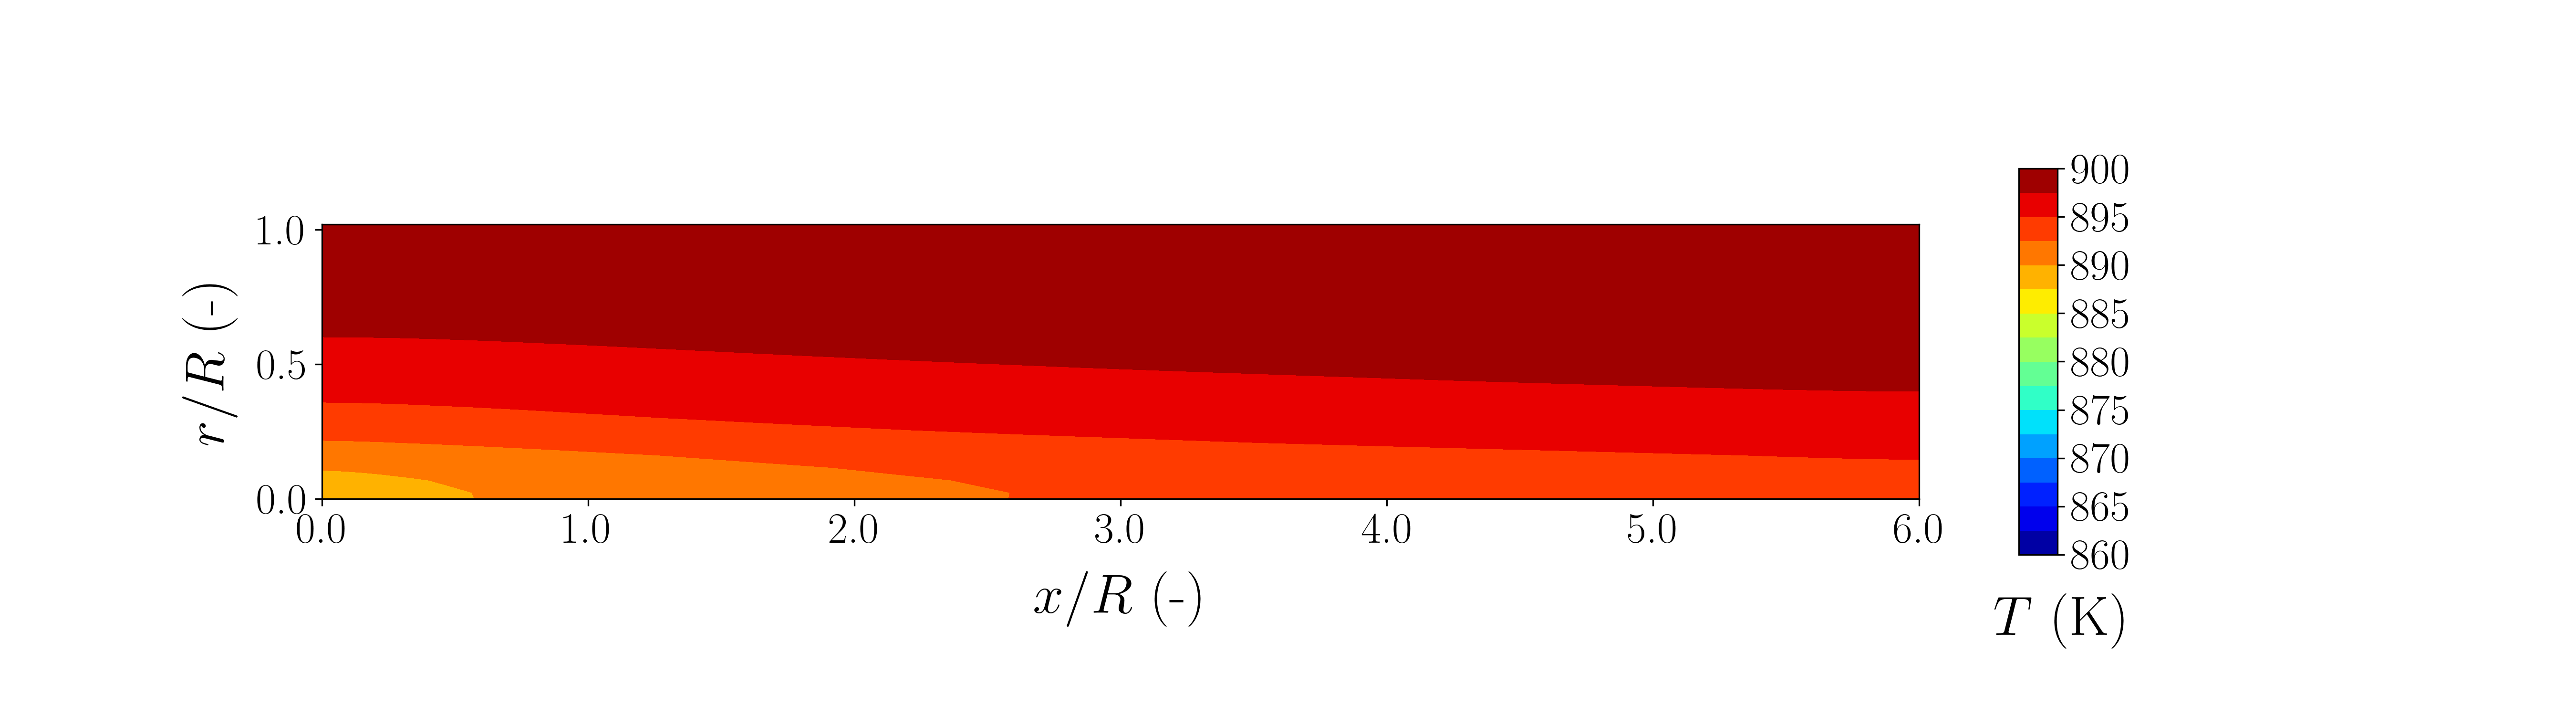
\includegraphics[width=190mm]{results/5/80C_20T/GEN30-TFIELD.png}
%\caption{\label{fig:5R8020G30-TField} Strategy I - Temperature field distribution - 30$^{\rm{th}}$ generation ($w_{\rm{CH_4}} = 0.8, w_T = 0.2$, $T_{\rm{in}}$ = 900 K, $u_{\rm{in}}$ = 0.15 m s$^{-1}$, $SC$ = 2.0)}
%\end{figure}
%
%
%\begin{figure}[h!]
%\centering
%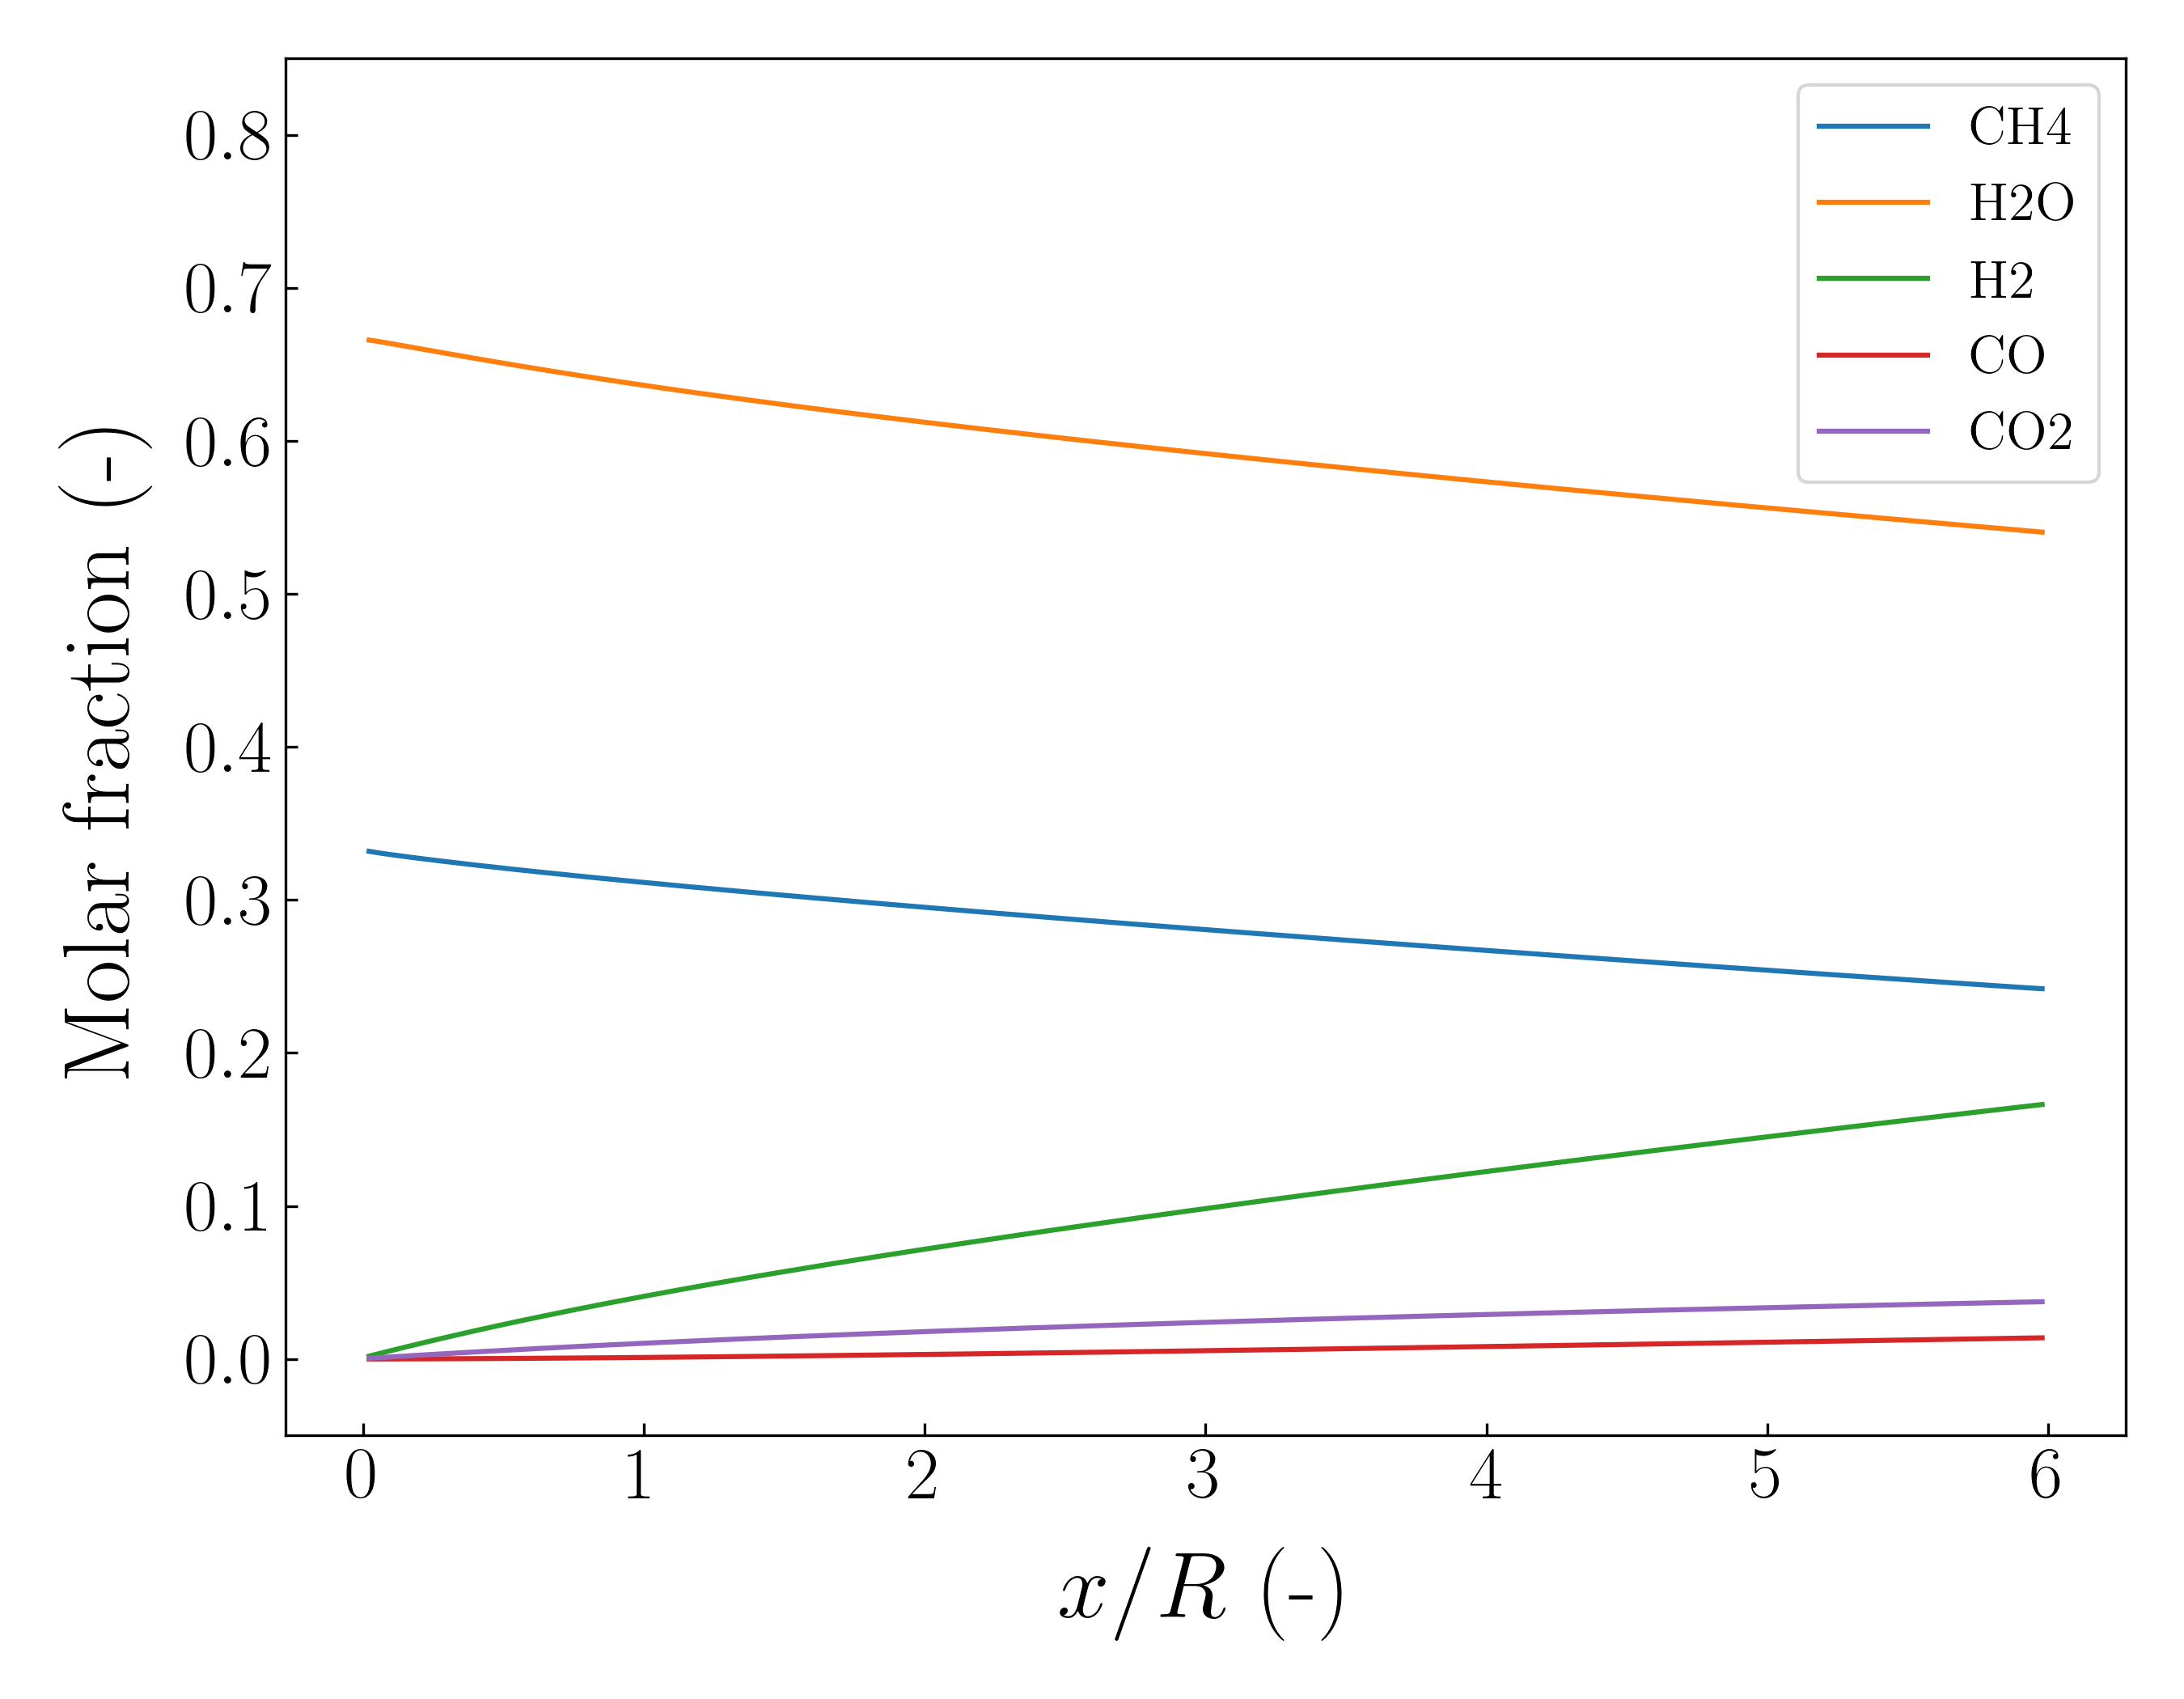
\includegraphics[width=80mm]{results/5/80C_20T/GEN1-AVG.png}
%\caption{\label{fig:5R8020G1-avg} Strategy I - Radius-averaged molar fractions - 1$^{\rm{st}}$ generation ($w_{\rm{CH_4}} = 0.8, w_T = 0.2$, $T_{\rm{in}}$ = 900 K, $u_{\rm{in}}$ = 0.15 m s$^{-1}$, $SC$ = 2.0)}
%\end{figure}
%
%\begin{figure}[h!]
%\centering
%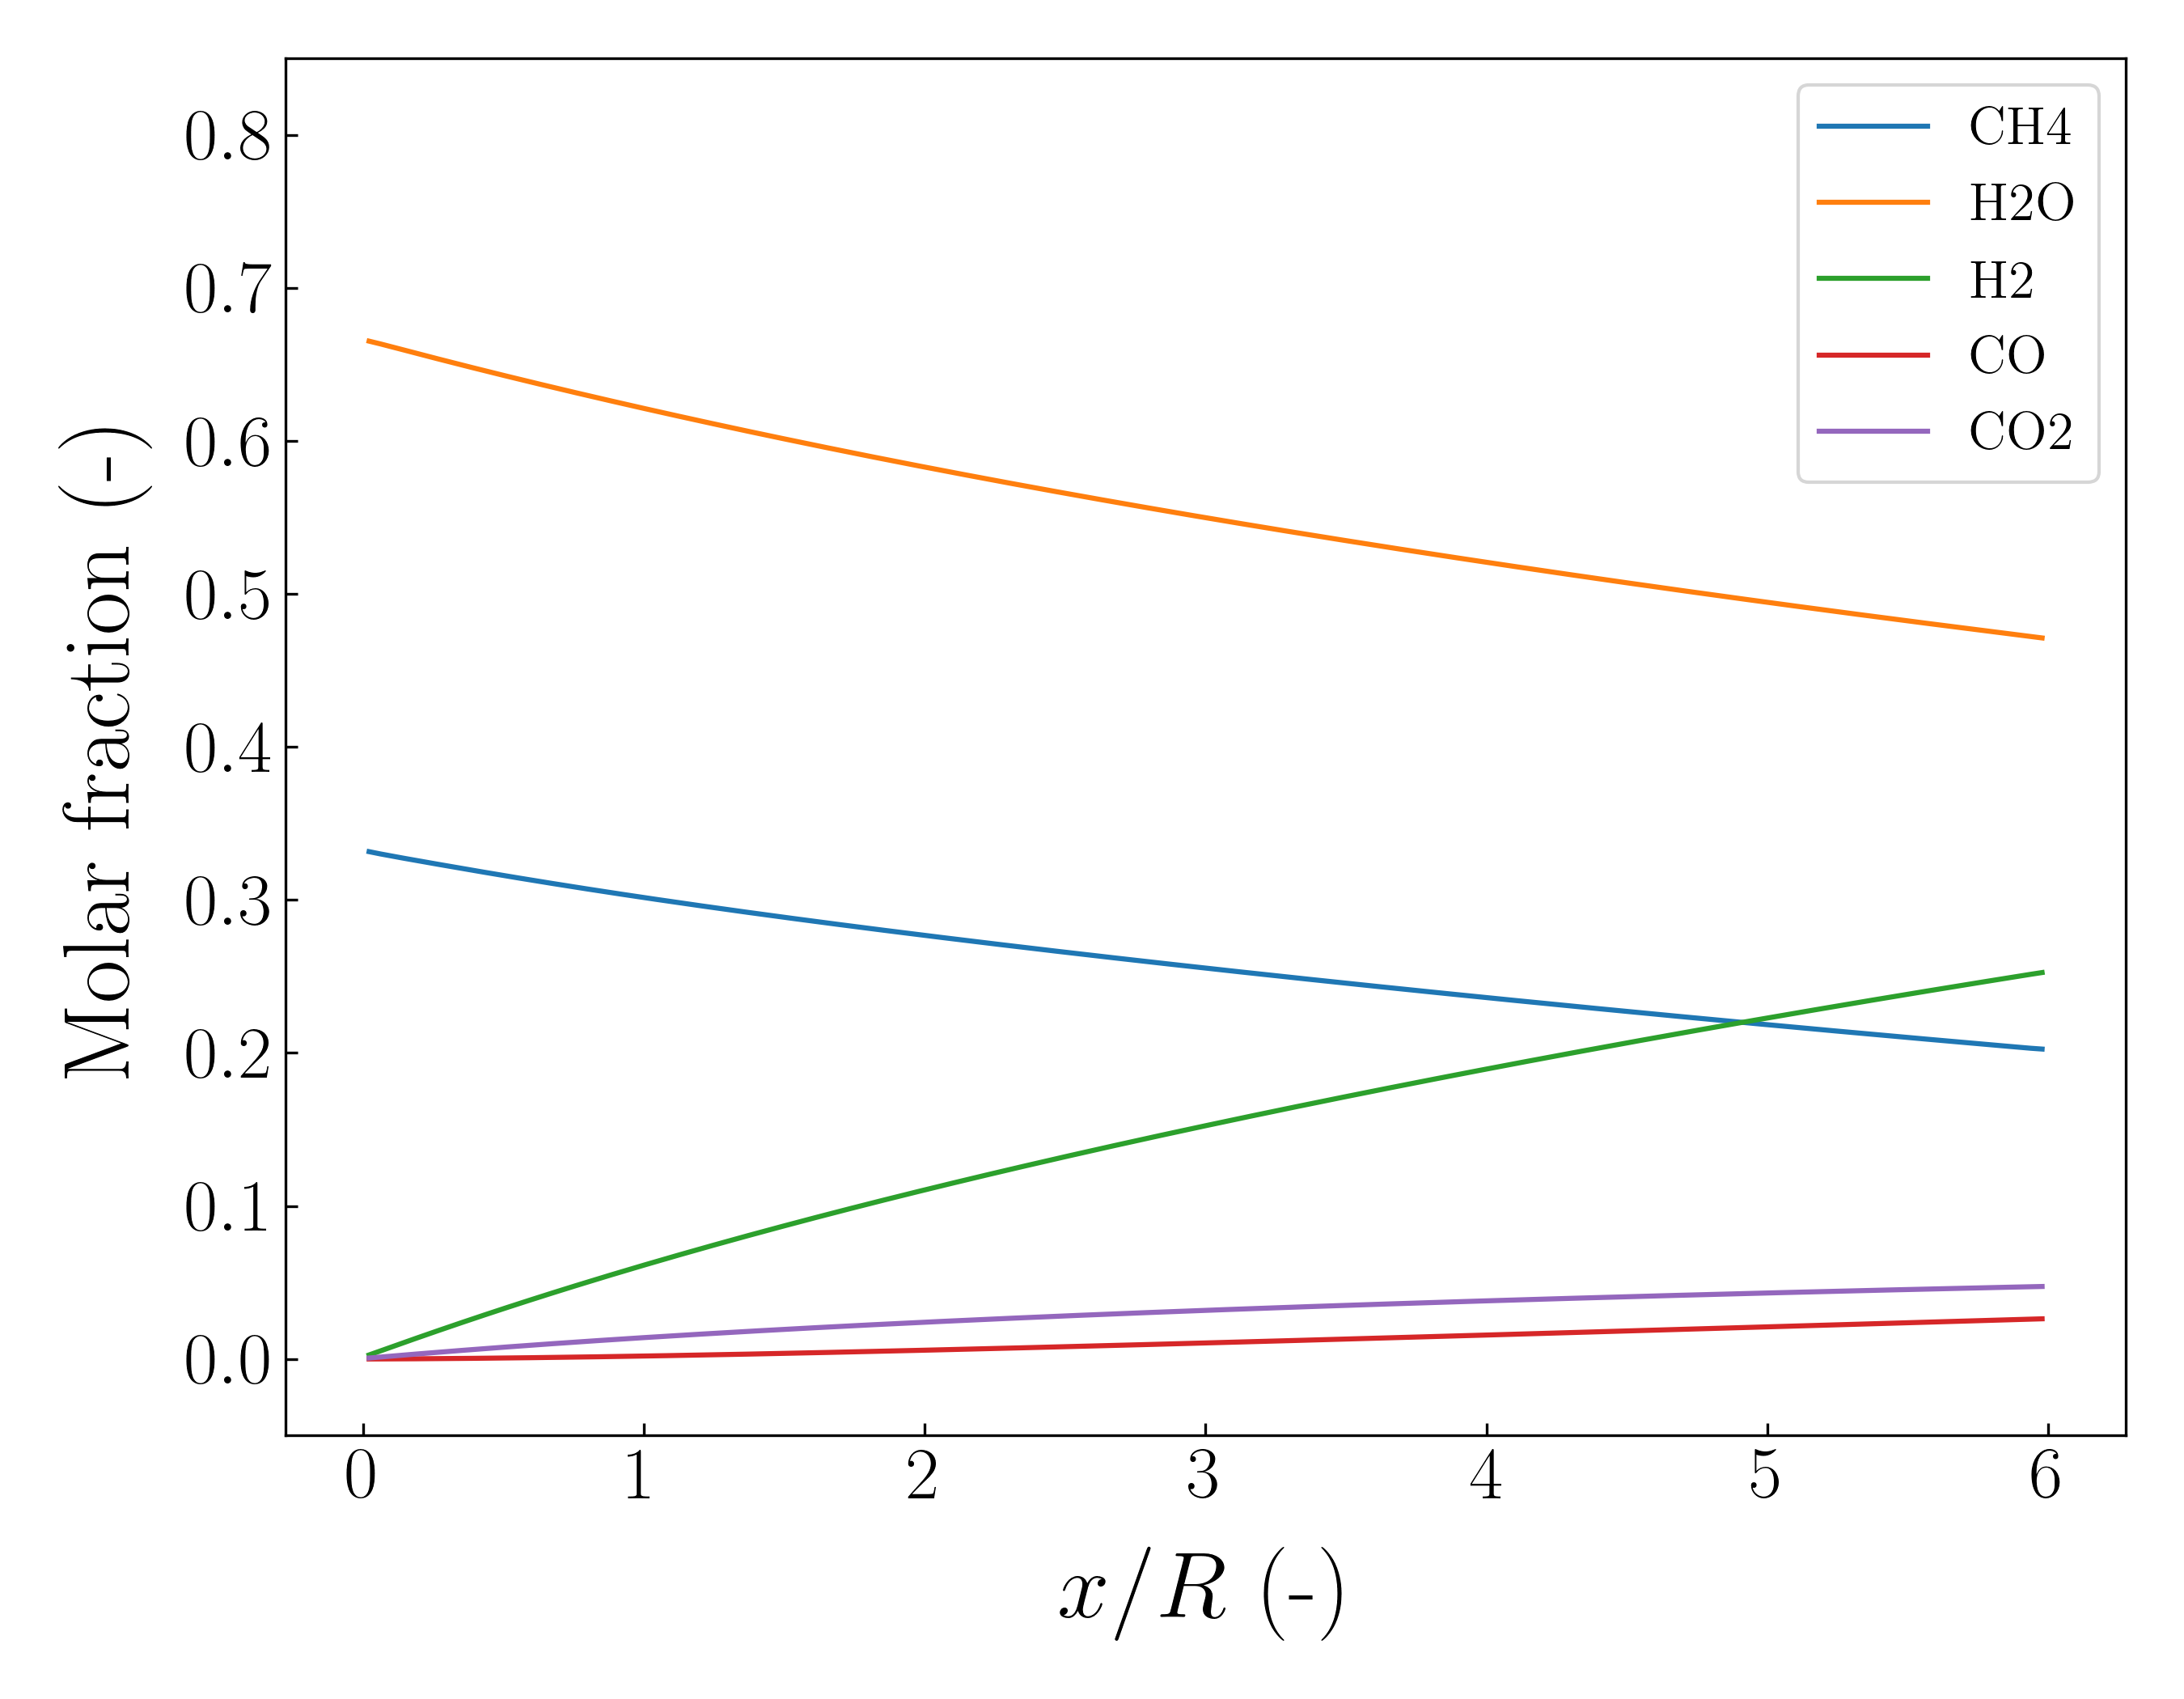
\includegraphics[width=80mm]{results/5/80C_20T/GEN15-AVG.png}
%\caption{\label{fig:5R8020G15-avg} Strategy I - Radius-averaged molar fractions - 15$^{\rm{th}}$ generation ($w_{\rm{CH_4}} = 0.8, w_T = 0.2$, $T_{\rm{in}}$ = 900 K, $u_{\rm{in}}$ = 0.15 m s$^{-1}$, $SC$ = 2.0)}
%\end{figure}
%
%\begin{figure}[h!]
%\centering
%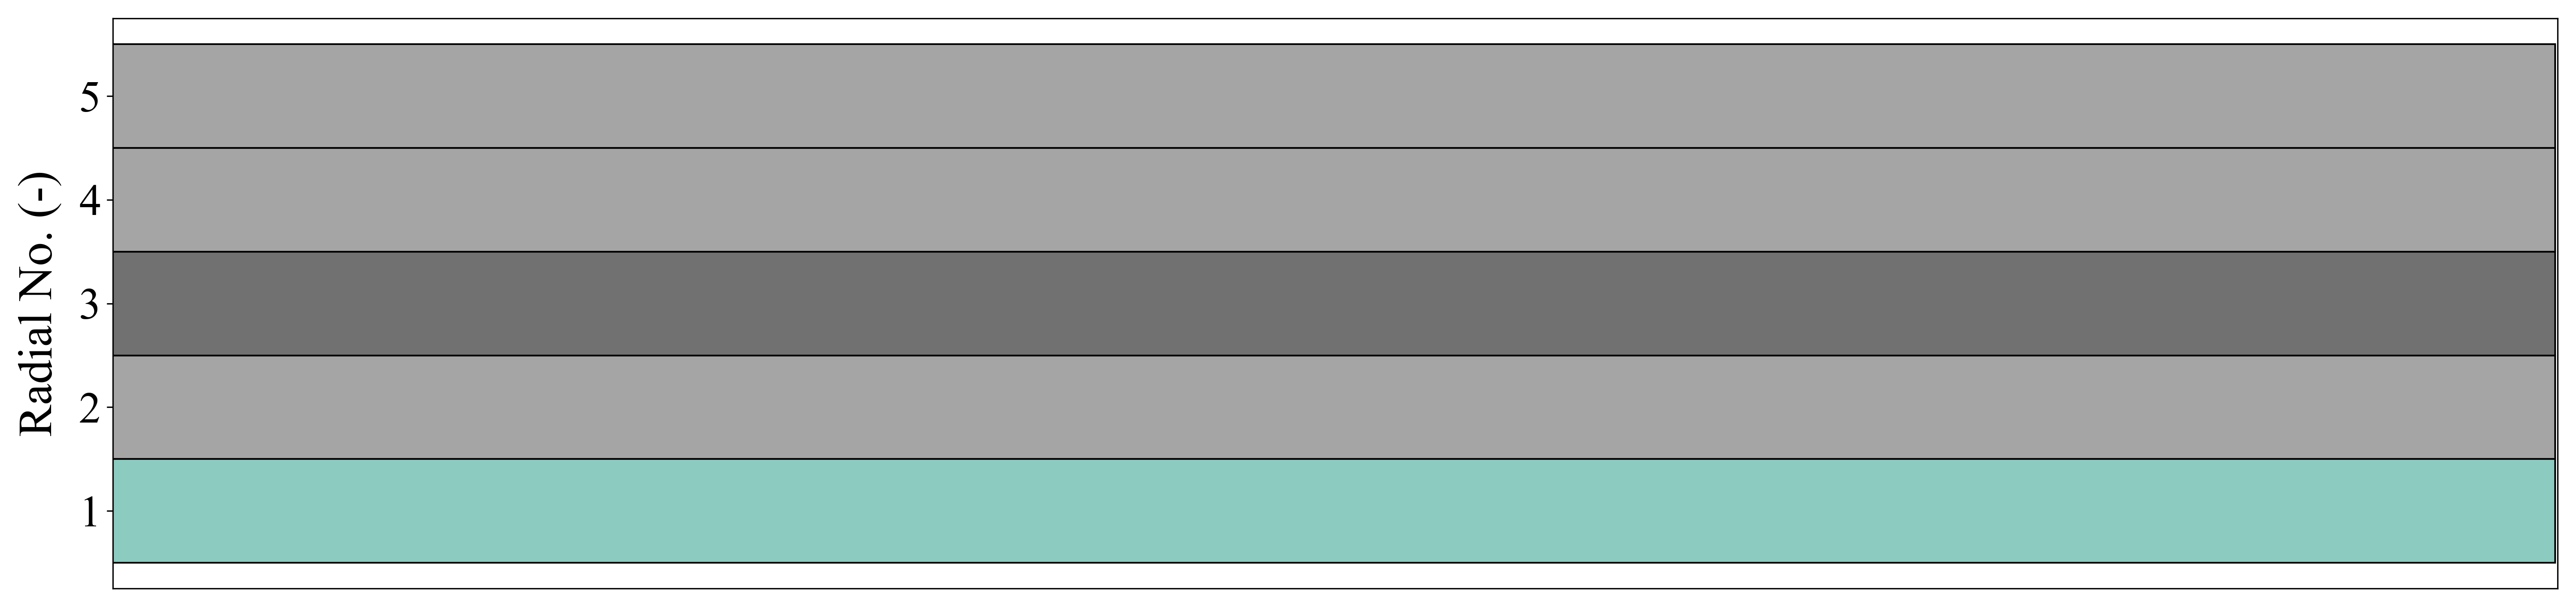
\includegraphics[width=120mm]{results/segments/5seg/80C20T/seg.png}
%\caption{\label{fig:30L6040G1-TField} Strategy I - Segments distribution for 30$^{\rm{th}}$ generation ($w_{\rm{CH_4}} = 0.8, w_T = 0.2$, $T_{\rm{in}}$ = 900 K, $u_{\rm{in}}$ = 0.15 m s$^{-1}$, $SC$ = 2.0)}
%\end{figure}
%
%\begin{figure}[h!]
%\centering
%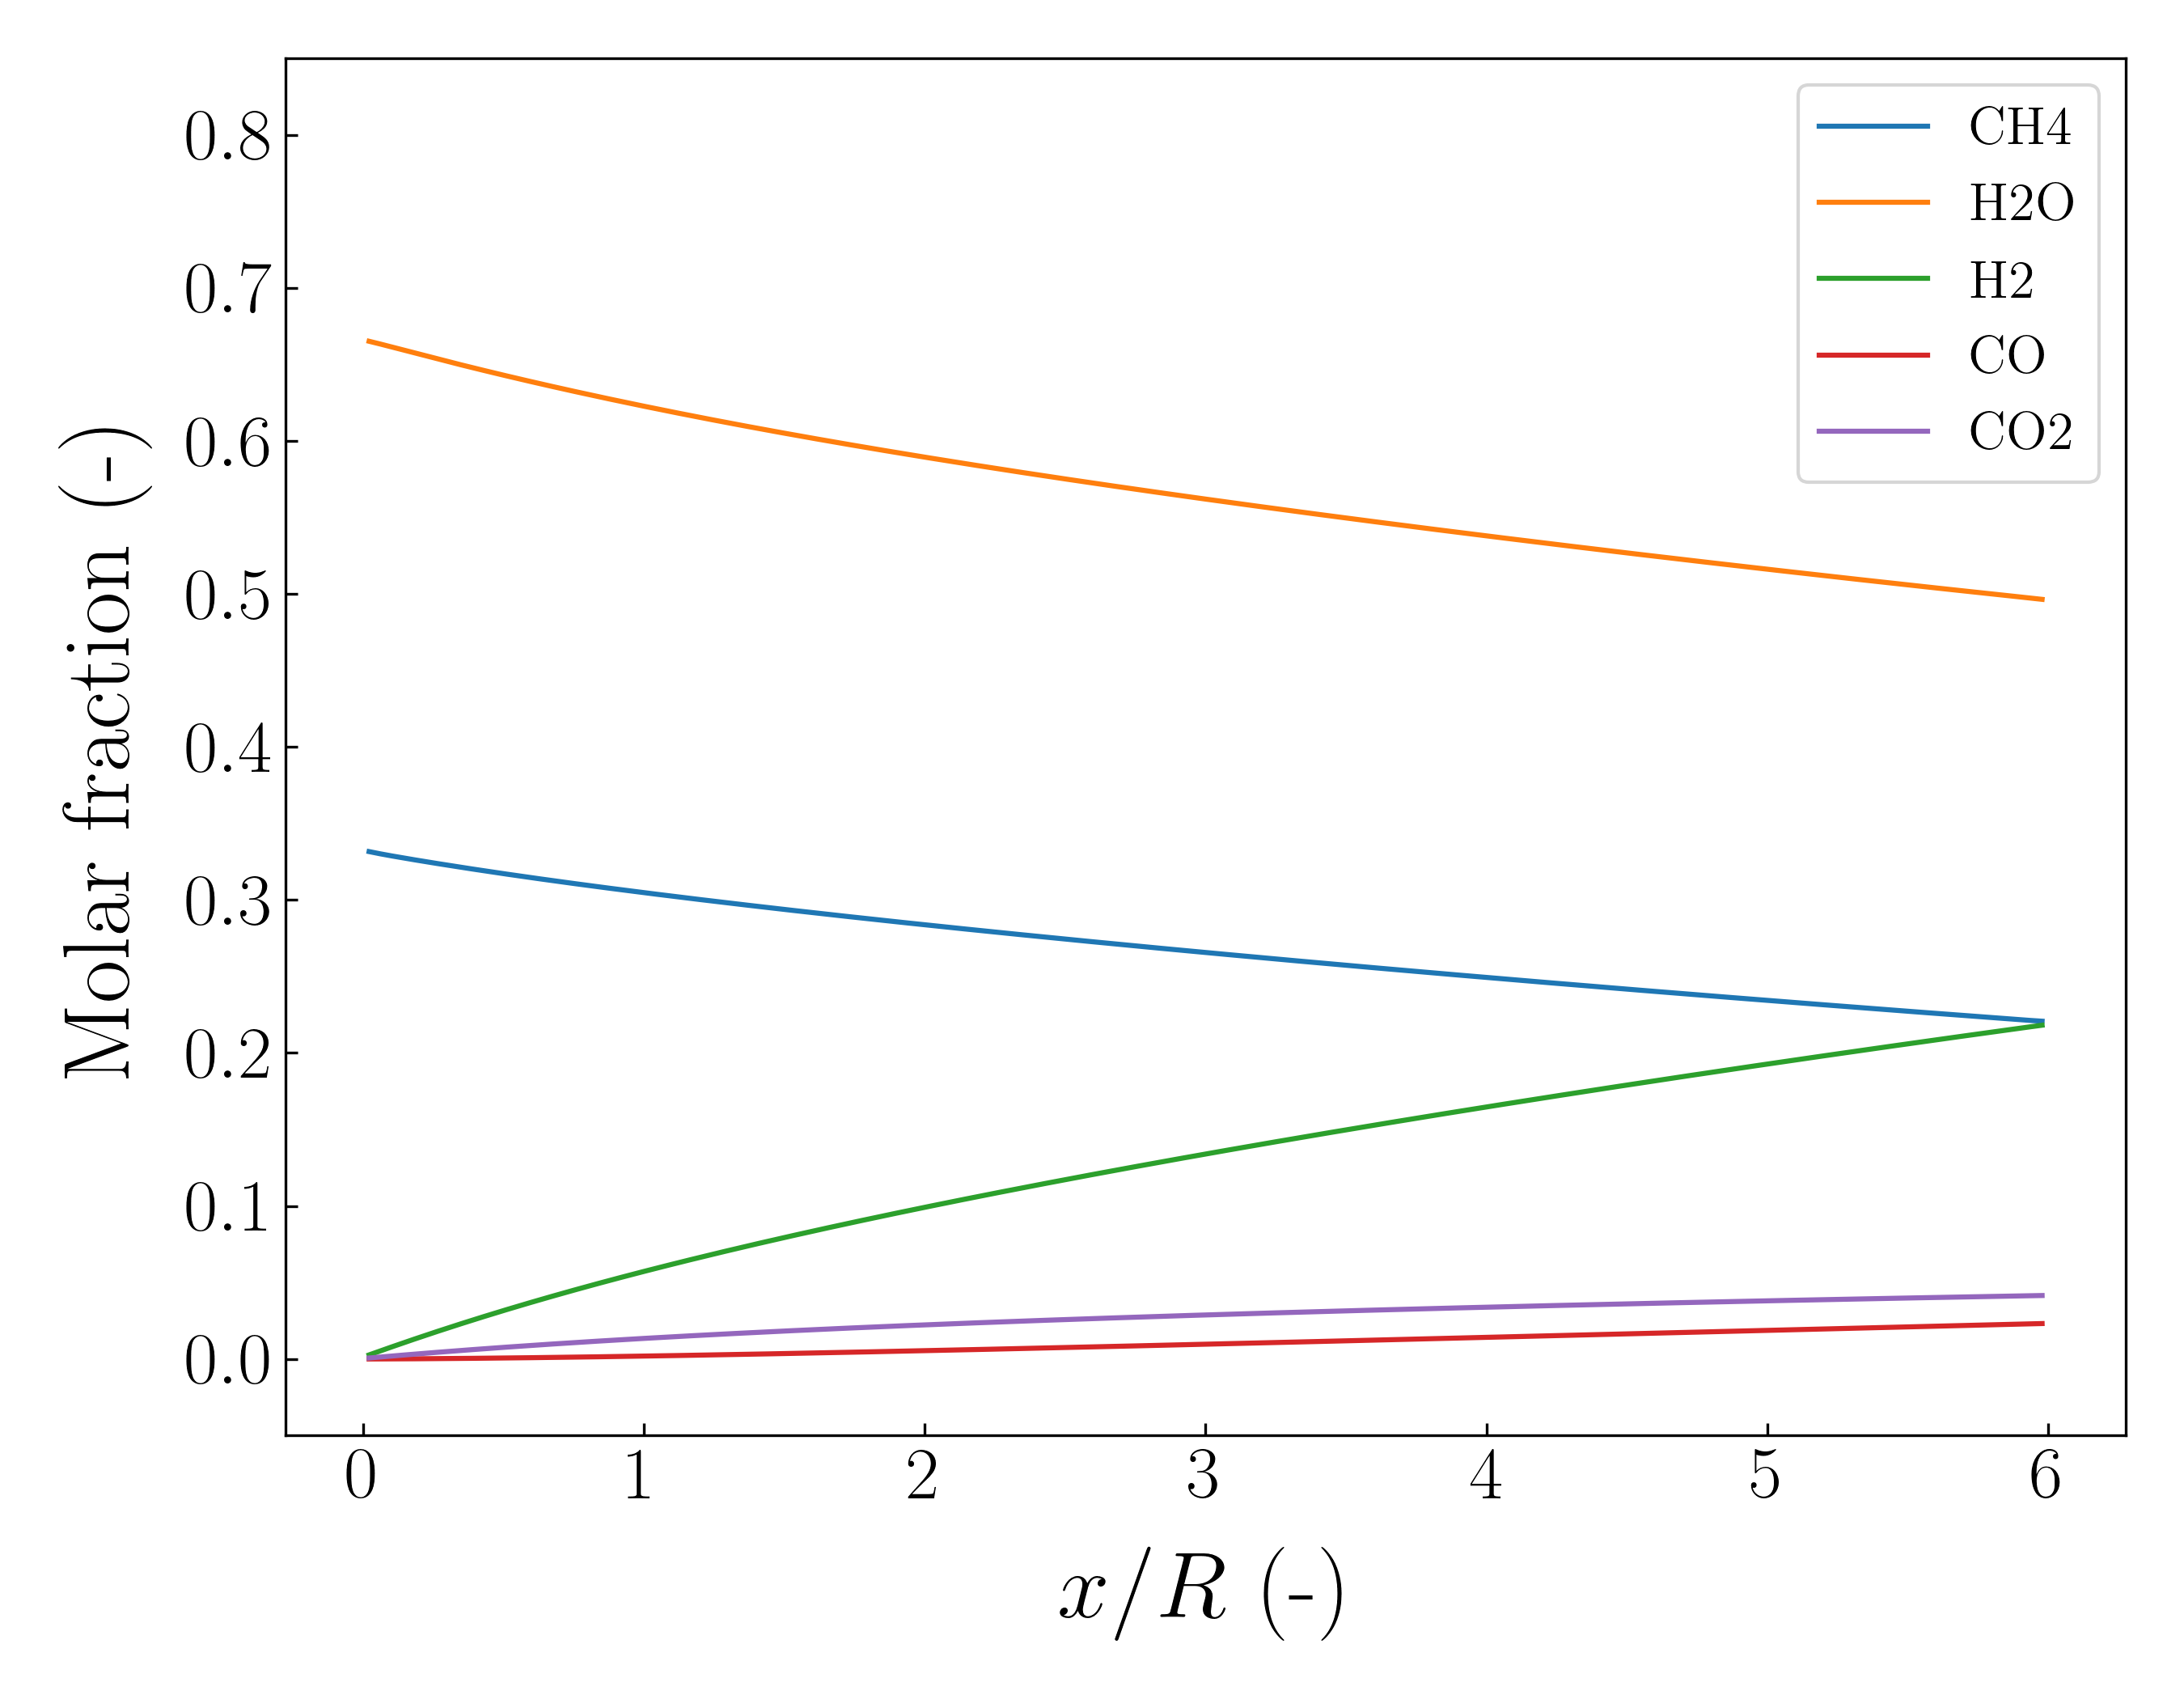
\includegraphics[width=80mm]{results/5/80C_20T/GEN30-AVG.png}
%\caption{\label{fig:5R8020G30-avg} Strategy I - Radius-averaged molar fractions -  30$^{\rm{th}}$ generation ($w_{\rm{CH_4}} = 0.8, w_T = 0.2$, $T_{\rm{in}}$ = 900 K, $u_{\rm{in}}$ = 0.15 m s$^{-1}$, $SC$ = 2.0)}
%\end{figure}
%
%
%The development of the fitness values among successive populations for strategy I is presented in Fig. \ref{fig:5R8020G-fitness}. 
%
%\begin{figure}
%\centering
%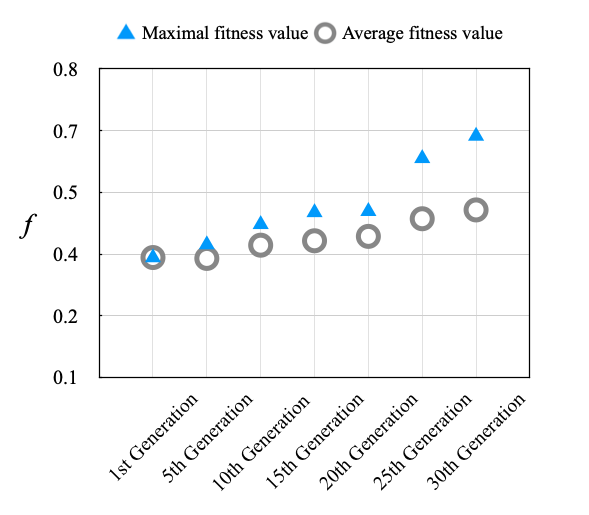
\includegraphics[width=100mm]{results/5/80C_20T.png}
%\caption{\label{fig:5R8020G-fitness} Strategy I - Fitness analysis throughout successive populations ($w_{\rm{CH_4}} = 0.8, w_T = 0.2$, $T_{\rm{in}}$ = 900 K, $u_{\rm{in}}$ = 0.15 m s$^{-1}$, $SC$ = 2.0)}
%\end{figure}
%
%To allow a straightforward comparison between the catalyst inserts division strategies, hydrogen productivity $\zeta$ is calculated for the optimal cases found by each algorithm. The hydrogen productivity is summarized in Table \ref{tab:5RH2prod}. 
%
%\begin{center}
%\begin{table}
%\centering
%\caption{Hydrogen productivity for the catalytic insert division strategy I}
%\label{tab:5RH2prod}
%\begin{tabular}{l|c|c|c}
%\hline\noalign{\smallskip}
% $w_{\rm{CH_4}}$ / $ w_T $ & $\rm{H_{2_{out}}}$ & $\iota$ & $\zeta$ \\
%\noalign{\smallskip}\hline\noalign{\smallskip}
%REF         & 0.581     & 1.00  &  0.581\\
%0.2 / 0.8   & 0.255     & 0.20  & 1.278 \\
%0.4 / 0.6   & 0.268     & 0.19  & 1.398 \\
%0.5 / 0.5   & 0.231     & 0.20  & 1.157 \\
%0.6 / 0.4   & 0.407     & 0.45  & 0.900 \\
%0.8 / 0.2   & 0.218     & 0.20  & 1.090 \\
%\noalign{\smallskip}\hline
%\end{tabular}
%\end{table}
%\end{center}
%
%
%\clearpage
%
%
%\subsection{Insert division strategy II}
%\label{subsec:5RE}
%
%\begin{figure}[h!]
%\centering
%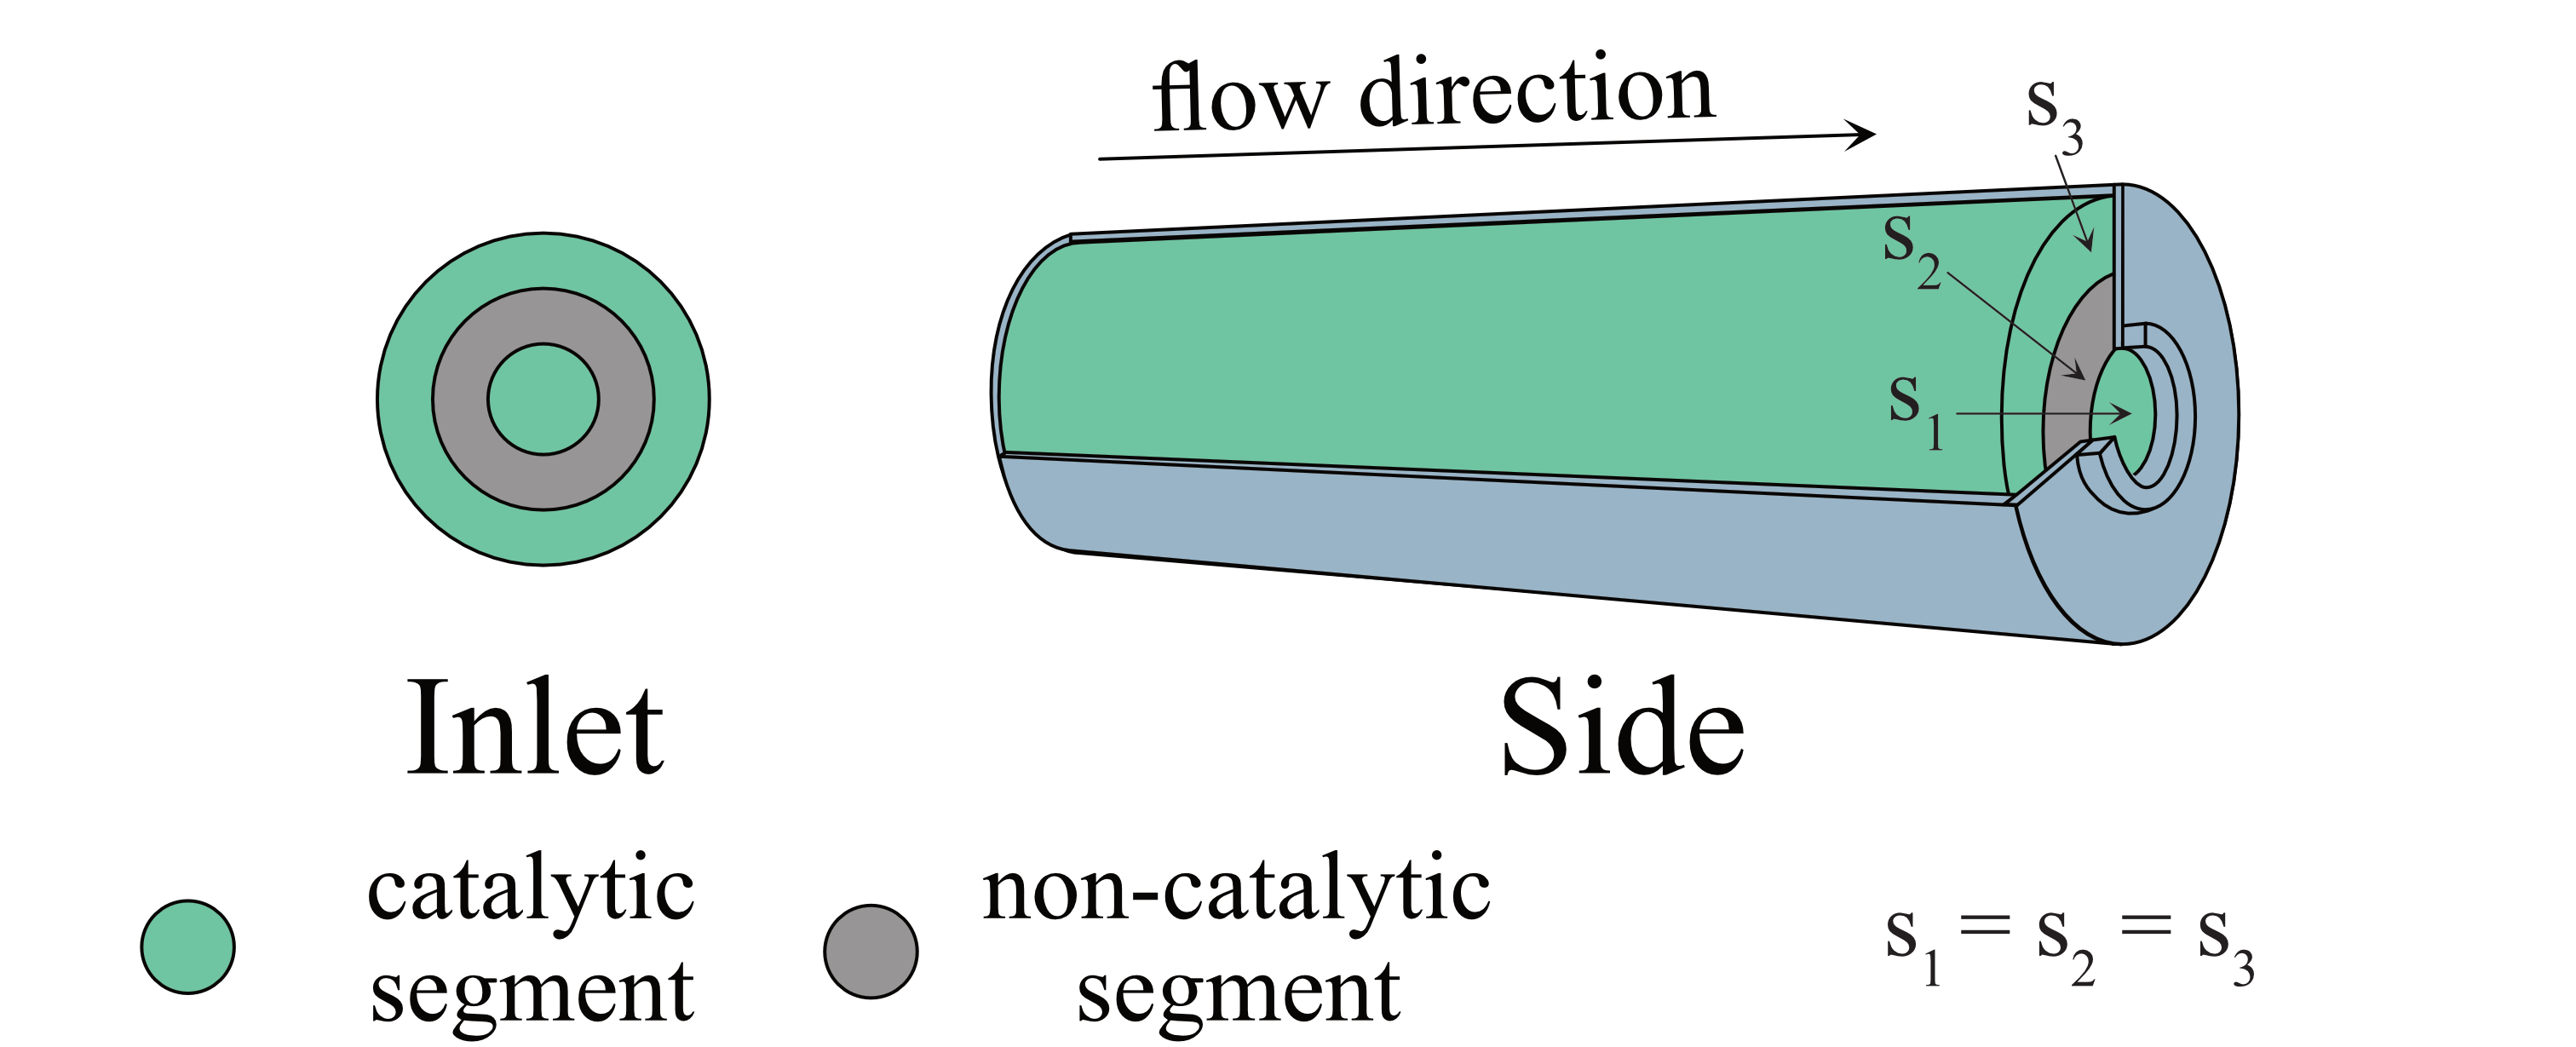
\includegraphics[width=120mm]{5segEqSurf.png}
%\caption{\label{fig:5segEqSurf}Catalytic insert division strategy II}
%\end{figure}
%
%
%\paragraph{Thermal fitness 80 \%, methane conversion 20 \%} \hspace{0pt} \\
%\noindent 
%
%
%\begin{figure}[h!]
%\centering
%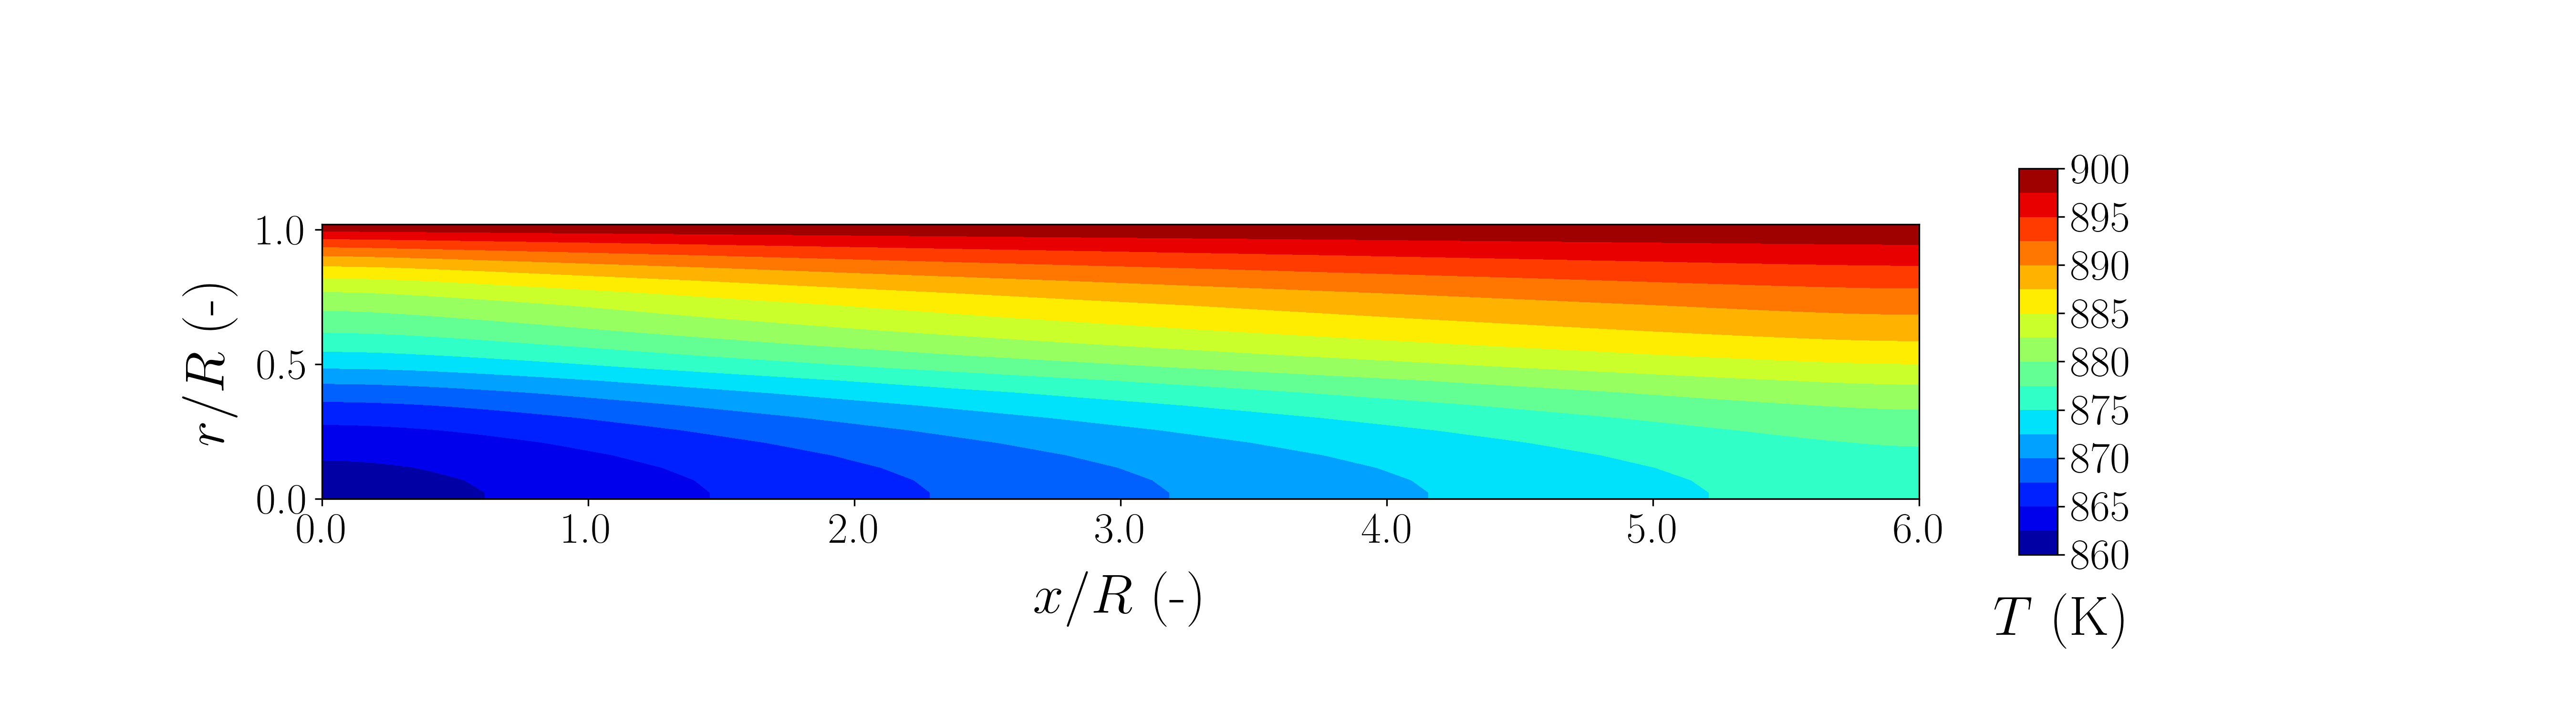
\includegraphics[width=190mm]{results/5Eq/20C_80T/GEN1-TFIELD.png}
%\caption{\label{fig:5RES2080G1-TField} Strategy II - Temperature field distribution - 1$^{\rm{st}}$ generation ($w_{\rm{CH_4}} = 0.2, w_T = 0.8$, $T_{\rm{in}}$ = 900 K, $u_{\rm{in}}$ = 0.15 m s$^{-1}$, $SC$ = 2.0)}
%\end{figure}
%
%\begin{figure}[h!]
%\centering
%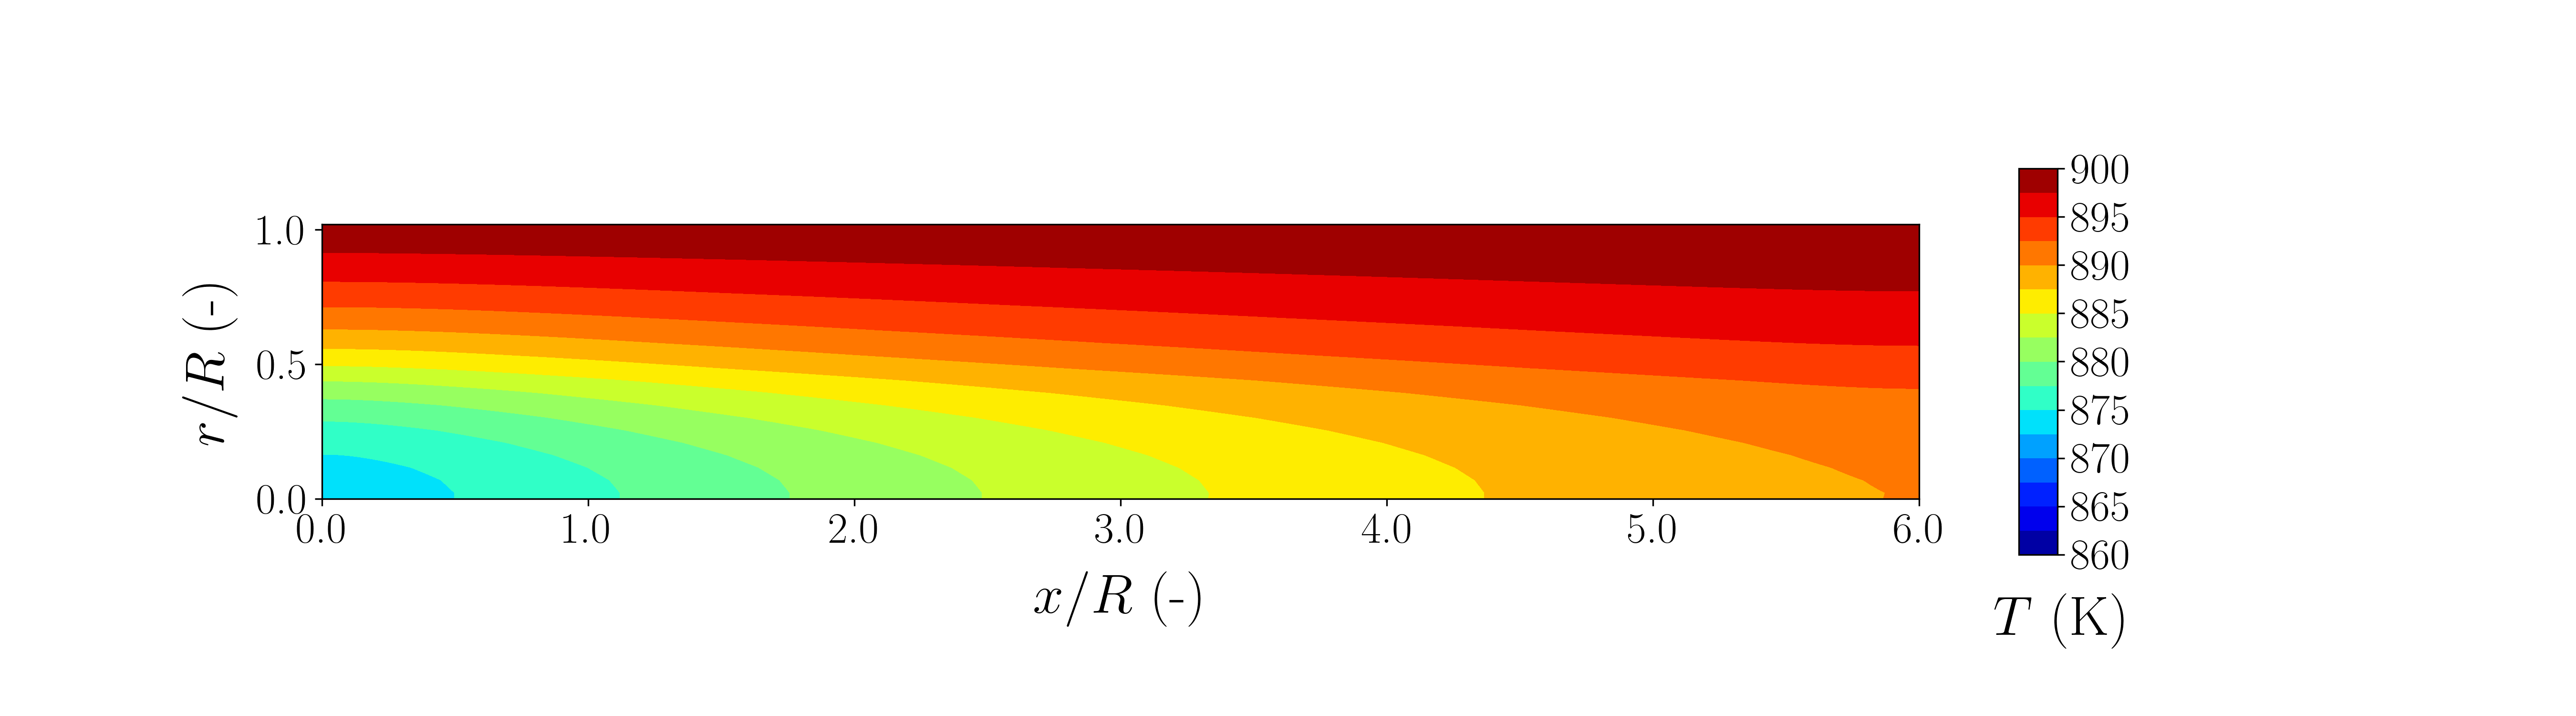
\includegraphics[width=190mm]{results/5Eq/20C_80T/GEN15-TFIELD.png}
%\caption{\label{fig:5RES2080G15-TField} Strategy II - Temperature field distribution - 15$^{\rm{th}}$ generation ($w_{\rm{CH_4}} = 0.2, w_T = 0.8$, $T_{\rm{in}}$ = 900 K, $u_{\rm{in}}$ = 0.15 m s$^{-1}$, $SC$ = 2.0)}
%\end{figure}
%
%\begin{figure}[h!]
%\centering
%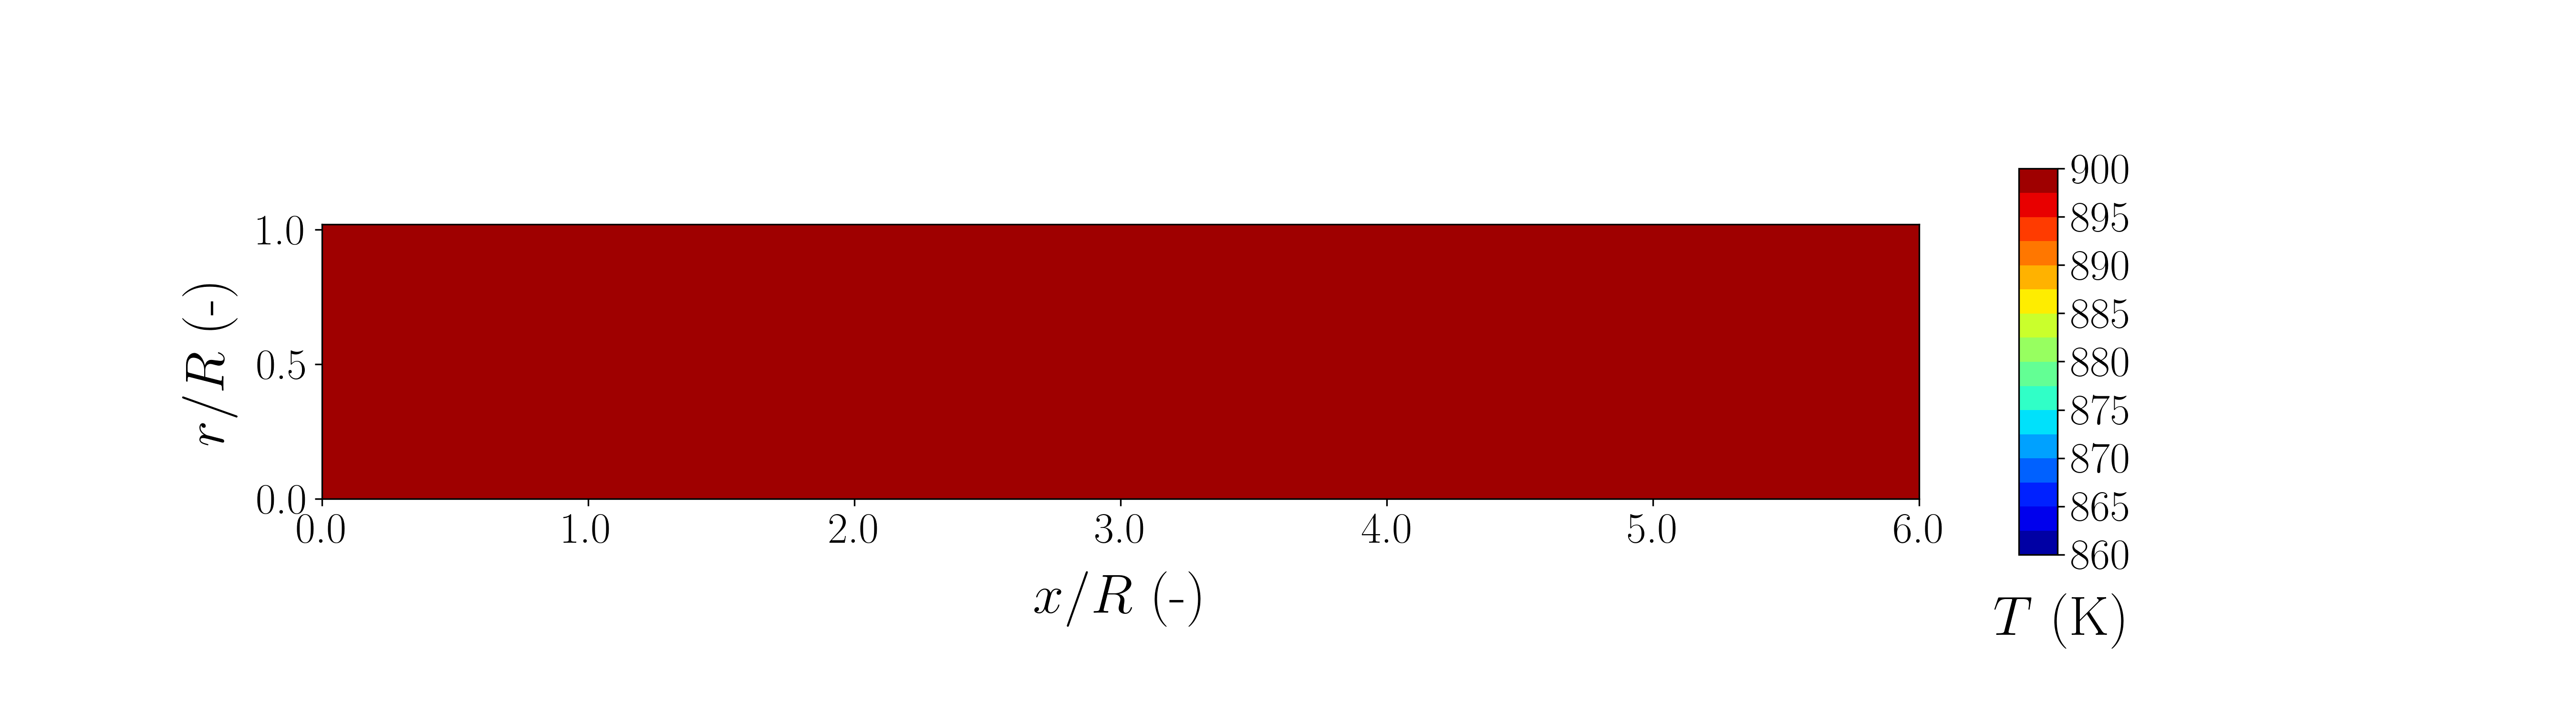
\includegraphics[width=190mm]{results/5Eq/20C_80T/GEN30-TFIELD.png}
%\caption{\label{fig:5RES2080G30-TField} Strategy II - Temperature field distribution - 30$^{\rm{th}}$ generation ($w_{\rm{CH_4}} = 0.2, w_T = 0.8$, $T_{\rm{in}}$ = 900 K, $u_{\rm{in}}$ = 0.15 m s$^{-1}$, $SC$ = 2.0)}
%\end{figure}
%
%
%\begin{figure}[h!]
%\centering
%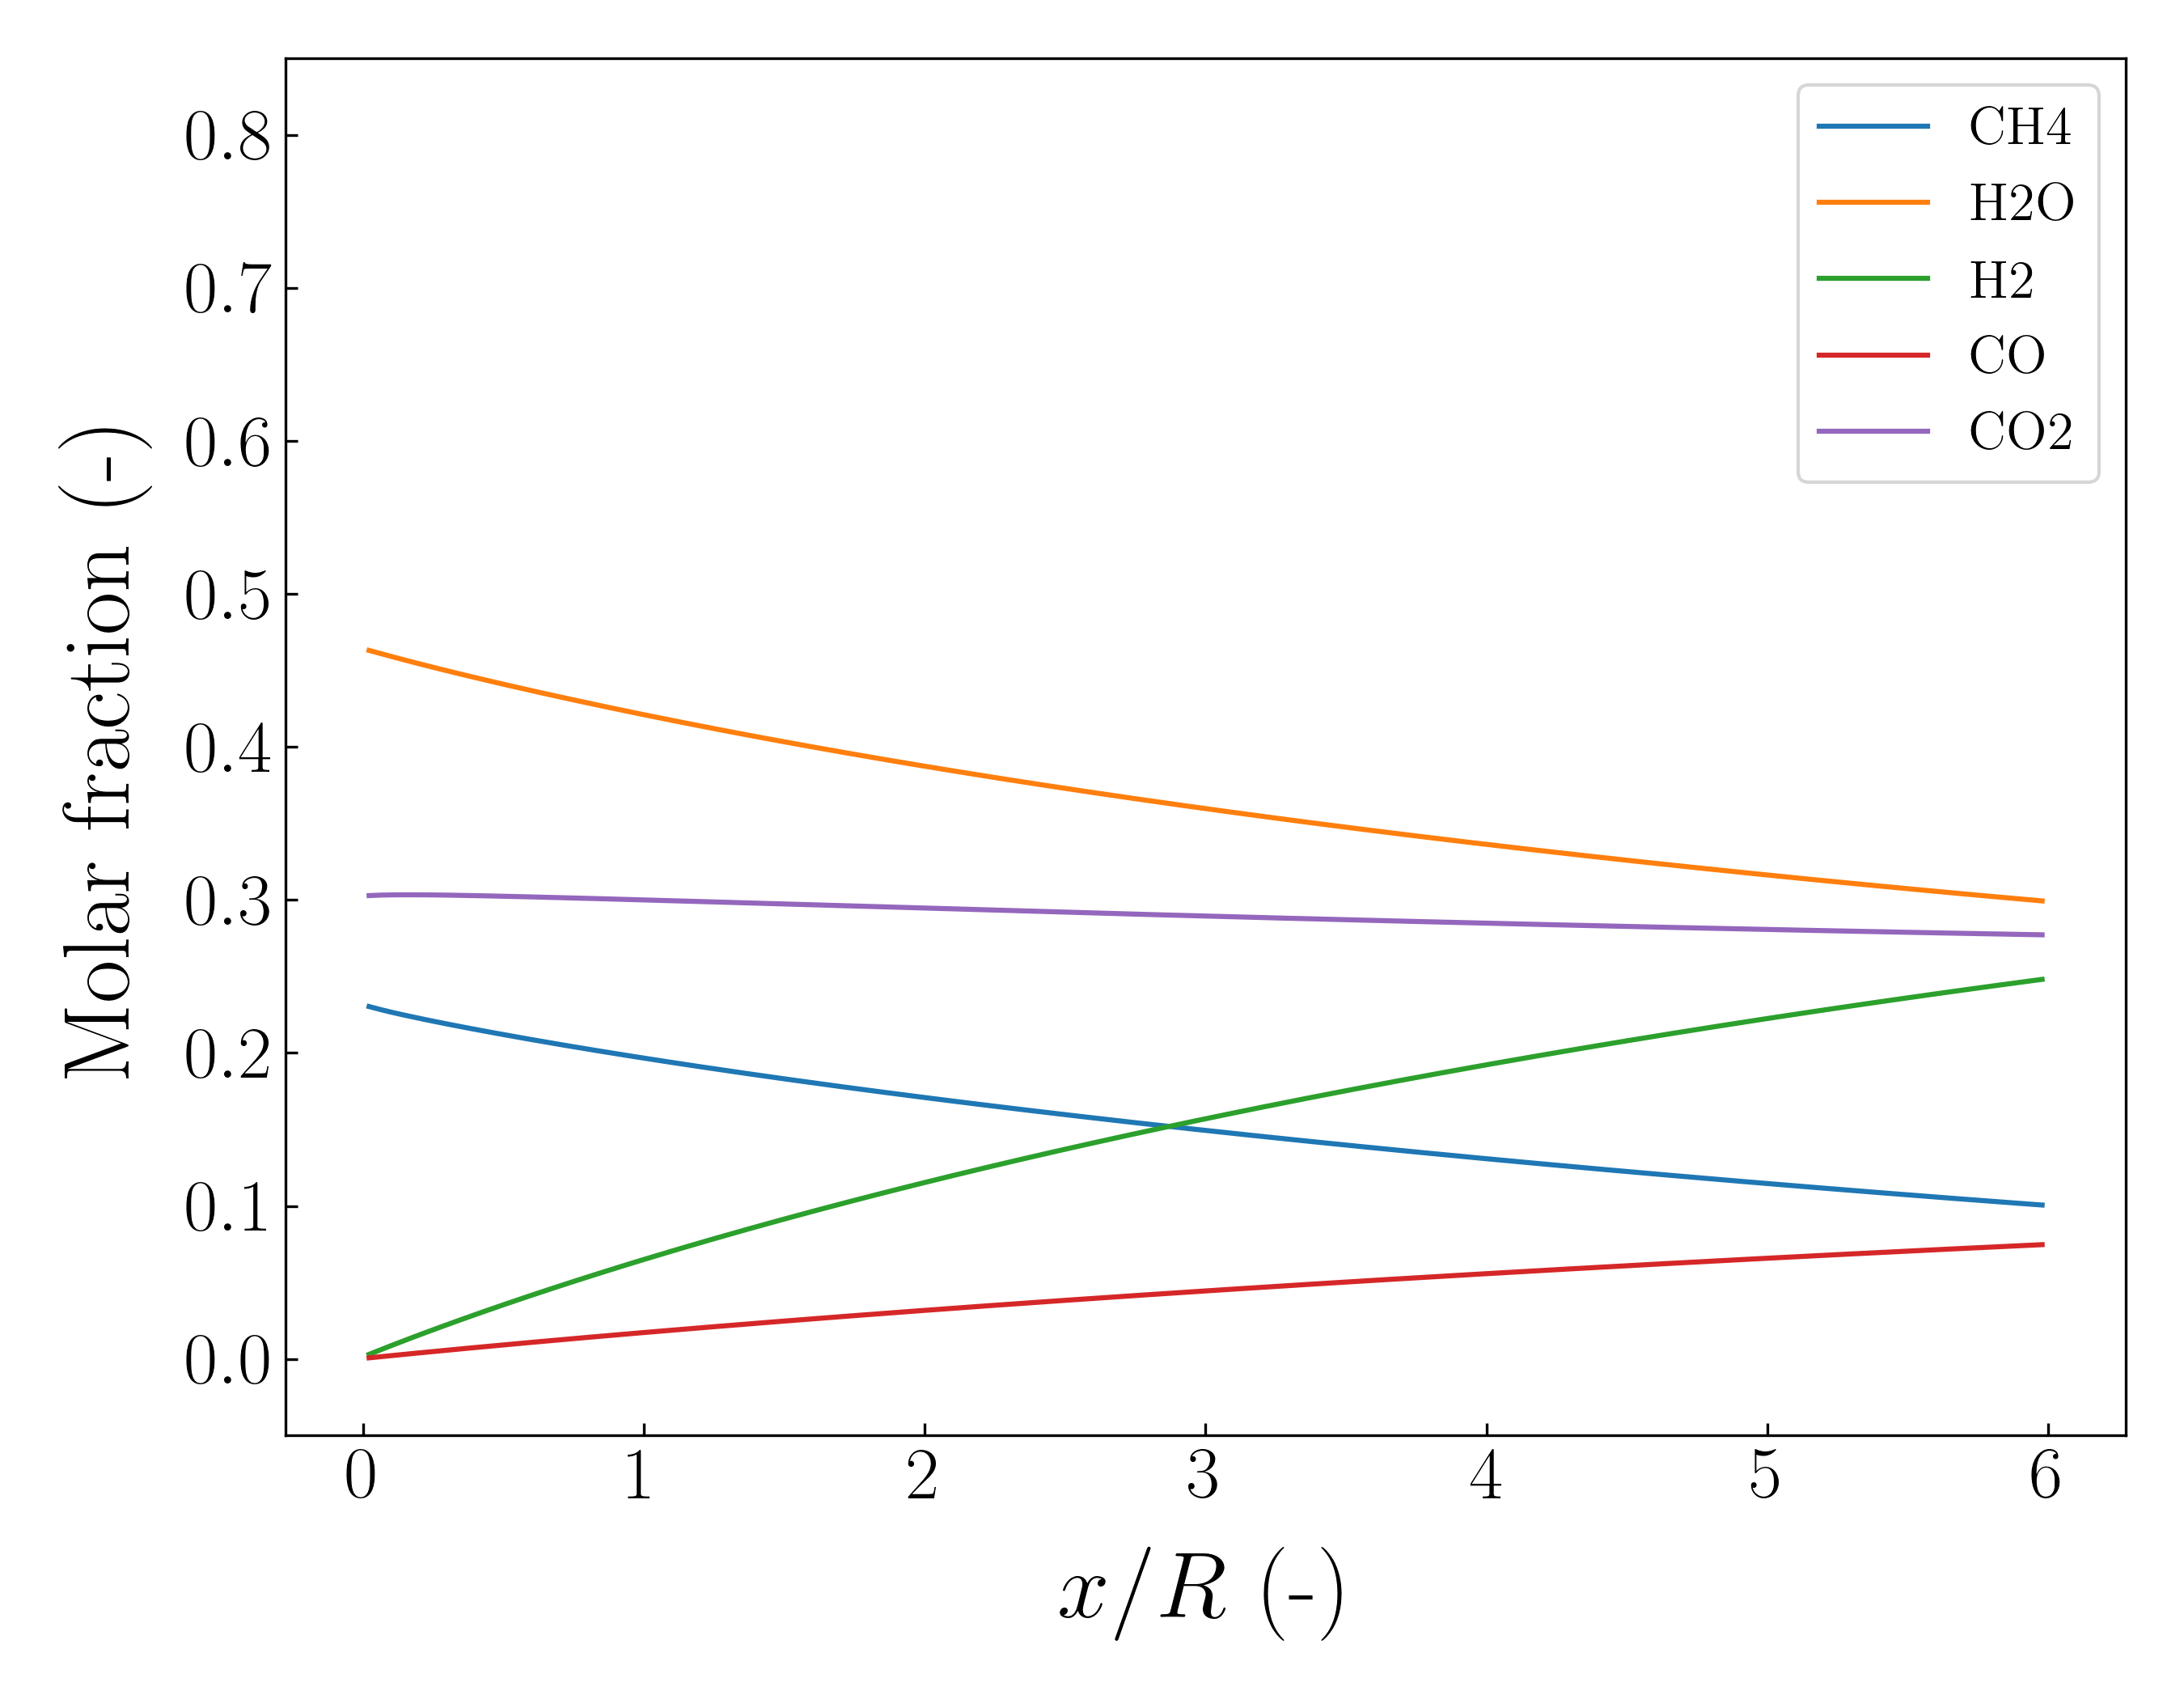
\includegraphics[width=80mm]{results/5Eq/20C_80T/GEN1-AVG.png}
%\caption{\label{fig:5RES2080G1-avg} Strategy II - Radius-averaged molar fractions - 1$^{\rm{st}}$ generation ($w_{\rm{CH_4}} = 0.2, w_T = 0.8$, $T_{\rm{in}}$ = 900 K, $u_{\rm{in}}$ = 0.15 m s$^{-1}$, $SC$ = 2.0)}
%\end{figure}
%
%\begin{figure}[h!]
%\centering
%\includegraphics[width=80mm]{results/5Eq/20C_80T/GEN15-AVG.png}
%\caption{\label{fig:5RES2080G15-avg} Strategy II - Radius-averaged molar fractions - 15$^{\rm{th}}$ generation ($w_{\rm{CH_4}} = 0.2, w_T = 0.8$, $T_{\rm{in}}$ = 900 K, $u_{\rm{in}}$ = 0.15 m s$^{-1}$, $SC$ = 2.0)}
%\end{figure}
%
%\begin{figure}[h!]
%\centering
%\includegraphics[width=80mm]{results/5Eq/20C_80T/GEN30-AVG.png}
%\caption{\label{fig:5RES2080G30-avg} Strategy II - Radius-averaged molar fractions -  30$^{\rm{th}}$ generation ($w_{\rm{CH_4}} = 0.2, w_T = 0.8$, $T_{\rm{in}}$ = 900 K, $u_{\rm{in}}$ = 0.15 m s$^{-1}$, $SC$ = 2.0)}
%\end{figure}
%
%\begin{figure}[h!]
%\centering
%\includegraphics[width=120mm]{results/segments/5segEq/20C80T/seg.png}
%\caption{\label{fig:30L6040G1-TField} Strategy II - Segments distribution for 30$^{\rm{th}}$ generation ($w_{\rm{CH_4}} = 0.2, w_T = 0.8$, $T_{\rm{in}}$ = 900 K, $u_{\rm{in}}$ = 0.15 m s$^{-1}$, $SC$ = 2.0)}
%\end{figure}
%
%\begin{figure}[h!]
%\centering
%\includegraphics[width=100mm]{results/5Eq/20C_80T.png}
%\caption{\label{fig:5RES2080G-fitness} Strategy II - Fitness analysis throughout successive populations ($w_{\rm{CH_4}} = 0.2, w_T = 0.8$, $T_{\rm{in}}$ = 900 K, $u_{\rm{in}}$ = 0.15 m s$^{-1}$, $SC$ = 2.0)}
%\end{figure}
%
%
%
%\clearpage
%
%
%
%\paragraph{Thermal fitness 60 \%, methane conversion 40 \%} \hspace{0pt} \\
%\noindent 
%
%
%\begin{figure}[h!]
%\centering
%\includegraphics[width=190mm]{results/5Eq/40C_60T/GEN1-TFIELD.png}
%\caption{\label{fig:5RES4060G1-TField} Strategy II - Temperature field distribution - 1$^{\rm{st}}$ generation ($w_{\rm{CH_4}} = 0.4, w_T = 0.6$, $T_{\rm{in}}$ = 900 K, $u_{\rm{in}}$ = 0.15 m s$^{-1}$, $SC$ = 2.0)}
%\end{figure}
%
%\begin{figure}[h!]
%\centering
%\includegraphics[width=190mm]{results/5Eq/40C_60T/GEN15-TFIELD.png}
%\caption{\label{fig:5RES4060G15-TField} Strategy II - Temperature field distribution - 15$^{\rm{th}}$ generation ($w_{\rm{CH_4}} = 0.4, w_T = 0.6$, $T_{\rm{in}}$ = 900 K, $u_{\rm{in}}$ = 0.15 m s$^{-1}$, $SC$ = 2.0)}
%\end{figure}
%
%\begin{figure}[h!]
%\centering
%\includegraphics[width=190mm]{results/5Eq/40C_60T/GEN30-TFIELD.png}
%\caption{\label{fig:5RES4060G30-TField} Strategy II - Temperature field distribution - 30$^{\rm{th}}$ generation ($w_{\rm{CH_4}} = 0.4, w_T = 0.6$, $T_{\rm{in}}$ = 900 K, $u_{\rm{in}}$ = 0.15 m s$^{-1}$, $SC$ = 2.0)}
%\end{figure}
%
%
%\begin{figure}[h!]
%\centering
%\includegraphics[width=80mm]{results/5Eq/40C_60T/GEN1-AVG.png}
%\caption{\label{fig:5RES4060G1-avg} Strategy II - Radius-averaged molar fractions - 1$^{\rm{st}}$ generation ($w_{\rm{CH_4}} = 0.4, w_T = 0.6$, $T_{\rm{in}}$ = 900 K, $u_{\rm{in}}$ = 0.15 m s$^{-1}$, $SC$ = 2.0)}
%\end{figure}
%
%\begin{figure}[h!]
%\centering
%\includegraphics[width=80mm]{results/5Eq/40C_60T/GEN15-AVG.png}
%\caption{\label{fig:5RES4060G15-avg} Strategy II - Radius-averaged molar fractions - 15$^{\rm{th}}$ generation ($w_{\rm{CH_4}} = 0.4, w_T = 0.6$, $T_{\rm{in}}$ = 900 K, $u_{\rm{in}}$ = 0.15 m s$^{-1}$, $SC$ = 2.0)}
%\end{figure}
%
%\begin{figure}[h!]
%\centering
%\includegraphics[width=80mm]{results/5Eq/40C_60T/GEN30-AVG.png}
%\caption{\label{fig:5RES4060G30-avg} Strategy II - Radius-averaged molar fractions -  30$^{\rm{th}}$ generation ($w_{\rm{CH_4}} = 0.4, w_T = 0.6$, $T_{\rm{in}}$ = 900 K, $u_{\rm{in}}$ = 0.15 m s$^{-1}$, $SC$ = 2.0)}
%\end{figure}
%
%\begin{figure}[h!]
%\centering
%\includegraphics[width=120mm]{results/segments/5segEq/40C60T/seg.png}
%\caption{\label{fig:30L6040G1-TField} Strategy II - Segments distribution for 30$^{\rm{th}}$ generation ($w_{\rm{CH_4}} = 0.4, w_T = 0.6$, $T_{\rm{in}}$ = 900 K, $u_{\rm{in}}$ = 0.15 m s$^{-1}$, $SC$ = 2.0)}
%\end{figure}
%
%\begin{figure}[h!]
%\centering
%\includegraphics[width=100mm]{results/5Eq/40C_60T.png}
%\caption{\label{fig:5RES4060G-fitness} Strategy II - Fitness analysis throughout successive populations ($w_{\rm{CH_4}} = 0.4, w_T = 0.6$, $T_{\rm{in}}$ = 900 K, $u_{\rm{in}}$ = 0.15 m s$^{-1}$, $SC$ = 2.0)}
%\end{figure}
%
%
%\clearpage
%
%
%
%
%
%\paragraph{Thermal fitness 50 \%, methane conversion 50 \%} \hspace{0pt} \\
%\noindent 
%
%
%\begin{figure}[h!]
%\centering
%\includegraphics[width=190mm]{results/5Eq/50C_50T/GEN1-TFIELD.png}
%\caption{\label{fig:5RES5050G1-TField} Strategy II - Temperature field distribution - 1$^{\rm{st}}$ generation ($w_{\rm{CH_4}} = 0.5, w_T = 0.5$, $T_{\rm{in}}$ = 900 K, $u_{\rm{in}}$ = 0.15 m s$^{-1}$, $SC$ = 2.0)}
%\end{figure}
%
%\begin{figure}[h!]
%\centering
%\includegraphics[width=190mm]{results/5Eq/50C_50T/GEN15-TFIELD.png}
%\caption{\label{fig:5RES5050G15-TField} Strategy II - Temperature field distribution - 15$^{\rm{th}}$ generation ($w_{\rm{CH_4}} = 0.5, w_T = 0.5$, $T_{\rm{in}}$ = 900 K, $u_{\rm{in}}$ = 0.15 m s$^{-1}$, $SC$ = 2.0)}
%\end{figure}
%
%\begin{figure}[h!]
%\centering
%\includegraphics[width=190mm]{results/5Eq/50C_50T/GEN30-TFIELD.png}
%\caption{\label{fig:5RES5050G30-TField} Strategy II - Temperature field distribution - 30$^{\rm{th}}$ generation ($w_{\rm{CH_4}} = 0.5, w_T = 0.5$, $T_{\rm{in}}$ = 900 K, $u_{\rm{in}}$ = 0.15 m s$^{-1}$, $SC$ = 2.0)}
%\end{figure}
%
%
%\begin{figure}[h!]
%\centering
%\includegraphics[width=80mm]{results/5Eq/50C_50T/GEN1-AVG.png}
%\caption{\label{fig:5RES5050G1-avg} Strategy II - Radius-averaged molar fractions - 1$^{\rm{st}}$ generation ($w_{\rm{CH_4}} = 0.5, w_T = 0.5$, $T_{\rm{in}}$ = 900 K, $u_{\rm{in}}$ = 0.15 m s$^{-1}$, $SC$ = 2.0)}
%\end{figure}
%
%\begin{figure}[h!]
%\centering
%\includegraphics[width=80mm]{results/5Eq/50C_50T/GEN15-AVG.png}
%\caption{\label{fig:5RES5050G15-avg} Strategy II - Radius-averaged molar fractions - 15$^{\rm{th}}$ generation ($w_{\rm{CH_4}} = 0.5, w_T = 0.5$, $T_{\rm{in}}$ = 900 K, $u_{\rm{in}}$ = 0.15 m s$^{-1}$, $SC$ = 2.0)}
%\end{figure}
%
%\begin{figure}[h!]
%\centering
%\includegraphics[width=80mm]{results/5Eq/50C_50T/GEN30-AVG.png}
%\caption{\label{fig:5RES5050G30-avg} Strategy II - Radius-averaged molar fractions -  30$^{\rm{th}}$ generation ($w_{\rm{CH_4}} = 0.5, w_T = 0.5$, $T_{\rm{in}}$ = 900 K, $u_{\rm{in}}$ = 0.15 m s$^{-1}$, $SC$ = 2.0)}
%\end{figure}
%
%\begin{figure}[h!]
%\centering
%\includegraphics[width=120mm]{results/segments/5segEq/50C50T/seg.png}
%\caption{\label{fig:30L6040G1-TField} Strategy II - Segments distribution for 30$^{\rm{th}}$ generation ($w_{\rm{CH_4}} = 0.5, w_T = 0.5$, $T_{\rm{in}}$ = 900 K, $u_{\rm{in}}$ = 0.15 m s$^{-1}$, $SC$ = 2.0)}
%\end{figure}
%
%
%\begin{figure}[h!]
%\centering
%\includegraphics[width=100mm]{results/5Eq/50C_50T.png}
%\caption{\label{fig:5RES5050G-fitness} Strategy II - Fitness analysis throughout successive populations ($w_{\rm{CH_4}} = 0.5, w_T = 0.5$, $T_{\rm{in}}$ = 900 K, $u_{\rm{in}}$ = 0.15 m s$^{-1}$, $SC$ = 2.0)}
%\end{figure}
%
%
%\clearpage
%
%
%
%\paragraph{Thermal fitness 40 \%, methane conversion 60 \%} \hspace{0pt} \\
%\noindent 
%
%
%\begin{figure}[h!]
%\centering
%\includegraphics[width=190mm]{results/5Eq/60C_40T/GEN1-TFIELD.png}
%\caption{\label{fig:5RES6040G1-TField} Strategy II - Temperature field distribution - 1$^{\rm{st}}$ generation ($w_{\rm{CH_4}} = 0.6, w_T = 0.4$, $T_{\rm{in}}$ = 900 K, $u_{\rm{in}}$ = 0.15 m s$^{-1}$, $SC$ = 2.0)}
%\end{figure}
%
%\begin{figure}[h!]
%\centering
%\includegraphics[width=190mm]{results/5Eq/60C_40T/GEN15-TFIELD.png}
%\caption{\label{fig:5RES6040G15-TField} Strategy II - Temperature field distribution - 15$^{\rm{th}}$ generation ($w_{\rm{CH_4}} = 0.6, w_T = 0.4$, $T_{\rm{in}}$ = 900 K, $u_{\rm{in}}$ = 0.15 m s$^{-1}$, $SC$ = 2.0)}
%\end{figure}
%
%\begin{figure}[h!]
%\centering
%\includegraphics[width=190mm]{results/5Eq/60C_40T/GEN30-TFIELD.png}
%\caption{\label{fig:5RES6040G30-TField} Strategy II - Temperature field distribution - 30$^{\rm{th}}$ generation ($w_{\rm{CH_4}} = 0.6, w_T = 0.4$, $T_{\rm{in}}$ = 900 K, $u_{\rm{in}}$ = 0.15 m s$^{-1}$, $SC$ = 2.0)}
%\end{figure}
%
%
%\begin{figure}[h!]
%\centering
%\includegraphics[width=80mm]{results/5Eq/60C_40T/GEN1-AVG.png}
%\caption{\label{fig:5RES6040G1-avg} Strategy II - Radius-averaged molar fractions - 1$^{\rm{st}}$ generation ($w_{\rm{CH_4}} = 0.6, w_T = 0.4$, $T_{\rm{in}}$ = 900 K, $u_{\rm{in}}$ = 0.15 m s$^{-1}$, $SC$ = 2.0)}
%\end{figure}
%
%\begin{figure}[h!]
%\centering
%\includegraphics[width=80mm]{results/5Eq/60C_40T/GEN15-AVG.png}
%\caption{\label{fig:5RES6040G15-avg} Strategy II - Radius-averaged molar fractions - 15$^{\rm{th}}$ generation ($w_{\rm{CH_4}} = 0.6, w_T = 0.4$, $T_{\rm{in}}$ = 900 K, $u_{\rm{in}}$ = 0.15 m s$^{-1}$, $SC$ = 2.0)}
%\end{figure}
%
%\begin{figure}[h!]
%\centering
%\includegraphics[width=80mm]{results/5Eq/60C_40T/GEN30-AVG.png}
%\caption{\label{fig:5RES6040G30-avg} Strategy II - Radius-averaged molar fractions -  30$^{\rm{th}}$ generation ($w_{\rm{CH_4}} = 0.6, w_T = 0.4$, $T_{\rm{in}}$ = 900 K, $u_{\rm{in}}$ = 0.15 m s$^{-1}$, $SC$ = 2.0)}
%\end{figure}
%
%\begin{figure}[h!]
%\centering
%\includegraphics[width=120mm]{results/segments/5segEq/60C40T/seg.png}
%\caption{\label{fig:30L6040G1-TField} Strategy II - Segments distribution for 30$^{\rm{th}}$ generation ($w_{\rm{CH_4}} = 0.6, w_T = 0.4$, $T_{\rm{in}}$ = 900 K, $u_{\rm{in}}$ = 0.15 m s$^{-1}$, $SC$ = 2.0)}
%\end{figure}
%
%\begin{figure}[h!]
%\centering
%\includegraphics[width=100mm]{results/5Eq/60C_40T.png}
%\caption{\label{fig:5RES6040G-fitness} Strategy II - Fitness analysis throughout successive populations ($w_{\rm{CH_4}} = 0.6, w_T = 0.4$, $T_{\rm{in}}$ = 900 K, $u_{\rm{in}}$ = 0.15 m s$^{-1}$, $SC$ = 2.0)}
%\end{figure}
%
%\clearpage
%
%
%\paragraph{Thermal fitness 20 \%, methane conversion 80 \%} \hspace{0pt} \\
%\noindent 
%
%
%
%\begin{figure}[h!]
%\centering
%\includegraphics[width=190mm]{results/5Eq/80C_20T/GEN1-TFIELD.png}
%\caption{\label{fig:5RES8020G1-TField} Strategy II - Temperature field distribution - 1$^{\rm{st}}$ generation ($w_{\rm{CH_4}} = 0.8, w_T = 0.2$, $T_{\rm{in}}$ = 900 K, $u_{\rm{in}}$ = 0.15 m s$^{-1}$, $SC$ = 2.0)}
%\end{figure}
%
%\begin{figure}[h!]
%\centering
%\includegraphics[width=190mm]{results/5Eq/80C_20T/GEN15-TFIELD.png}
%\caption{\label{fig:5RES8020G15-TField} Strategy II - Temperature field distribution - 15$^{\rm{th}}$ generation ($w_{\rm{CH_4}} = 0.8, w_T = 0.2$, $T_{\rm{in}}$ = 900 K, $u_{\rm{in}}$ = 0.15 m s$^{-1}$, $SC$ = 2.0)}
%\end{figure}
%
%\begin{figure}[h!]
%\centering
%\includegraphics[width=190mm]{results/5Eq/80C_20T/GEN30-TFIELD.png}
%\caption{\label{fig:5RES8020G30-TField} Strategy II - Temperature field distribution - 30$^{\rm{th}}$ generation ($w_{\rm{CH_4}} = 0.8, w_T = 0.2$, $T_{\rm{in}}$ = 900 K, $u_{\rm{in}}$ = 0.15 m s$^{-1}$, $SC$ = 2.0)}
%\end{figure}
%
%
%\begin{figure}[h!]
%\centering
%\includegraphics[width=80mm]{results/5Eq/80C_20T/GEN1-AVG.png}
%\caption{\label{fig:5RES8020G1-avg} Strategy II - Radius-averaged molar fractions - 1$^{\rm{st}}$ generation ($w_{\rm{CH_4}} = 0.8, w_T = 0.2$, $T_{\rm{in}}$ = 900 K, $u_{\rm{in}}$ = 0.15 m s$^{-1}$, $SC$ = 2.0)}
%\end{figure}
%
%\begin{figure}[h!]
%\centering
%\includegraphics[width=80mm]{results/5Eq/80C_20T/GEN15-AVG.png}
%\caption{\label{fig:5RES8020G15-avg} Strategy II - Radius-averaged molar fractions - 15$^{\rm{th}}$ generation ($w_{\rm{CH_4}} = 0.8, w_T = 0.2$, $T_{\rm{in}}$ = 900 K, $u_{\rm{in}}$ = 0.15 m s$^{-1}$, $SC$ = 2.0)}
%\end{figure}
%
%\begin{figure}[h!]
%\centering
%\includegraphics[width=120mm]{results/segments/5segEq/80C20T/seg.png}
%\caption{\label{fig:30L6040G1-TField} Strategy II - Segments distribution for 30$^{\rm{th}}$ generation ($w_{\rm{CH_4}} = 0.8, w_T = 0.2$, $T_{\rm{in}}$ = 900 K, $u_{\rm{in}}$ = 0.15 m s$^{-1}$, $SC$ = 2.0)}
%\end{figure}
%
%\begin{figure}[h!]
%\centering
%\includegraphics[width=80mm]{results/5Eq/80C_20T/GEN30-AVG.png}
%\caption{\label{fig:5RES8020G30-avg} Strategy II - Radius-averaged molar fractions -  30$^{\rm{th}}$ generation ($w_{\rm{CH_4}} = 0.8, w_T = 0.2$, $T_{\rm{in}}$ = 900 K, $u_{\rm{in}}$ = 0.15 m s$^{-1}$, $SC$ = 2.0)}
%\end{figure}
%
%
%\begin{figure}[h!]
%\centering
%\includegraphics[width=100mm]{results/5Eq/80C_20T.png}
%\caption{\label{fig:5RES8020G-fitness} Strategy II - Fitness analysis throughout successive populations ($w_{\rm{CH_4}} = 0.8, w_T = 0.2$, $T_{\rm{in}}$ = 900 K, $u_{\rm{in}}$ = 0.15 m s$^{-1}$, $SC$ = 2.0)}
%\end{figure}
%
%\begin{center}
%\begin{table}
%\centering
%\caption{Hydrogen productivity for the catalytic insert division strategy II}
%\label{tab:5RH2prod}
%\begin{tabular}{l|c|c|c}
%\hline\noalign{\smallskip}
% $w_{\rm{CH_4}}$ / $ w_T $ & $\rm{H_{2_{out}}}$ & $\iota$ & $\zeta$ \\
%\noalign{\smallskip}\hline\noalign{\smallskip}
%REF         & 0.581     & 1.00  &  0.581\\
%0.2 / 0.8   & 0.001     & 0.00  & N / A \\
%0.4 / 0.6   & 0.492     & 0.32  & 1.527 \\
%0.5 / 0.5   & 0.175     & 0.32  & 0.548 \\
%0.6 / 0.4   & 0.536     & 0.53  & 1.616 \\
%0.8 / 0.2   & 0.200     & 0.27  & 0.744 \\
%\noalign{\smallskip}\hline
%\end{tabular}
%\end{table}
%\end{center}

\section{Conclusions}


%% The Appendices part is started with the command \appendix;
%% appendix sections are then done as normal sections
%% \appendix

%% \section{}
%% \label{}

%% For citations use: 
%%       \citet{<label>} ==> Jones et al. [21]
%%       \citep{<label>} ==> [21]
%%

%% If you have bibdatabase file and want bibtex to generate the
%% bibitems, please use
%%

\clearpage

\bibliographystyle{elsarticle-num-names} 
\bibliography{bib1.bib}

%% else use the following coding to input the bibitems directly in the
%% TeX file.

\begin{thebibliography}{00}

%% \bibitem[Author(year)]{label}
%% Text of bibliographic item

%\bibitem[ ()]{}

\end{thebibliography}
\end{document}

\endinput
%%
%% End of file `elsarticle-template-num-names.tex'.
